\chapter{Modelado}

En este capítulo desarrollo el proceso de modelado de los datos franceses con tal de explorar las configuraciones sociales que favorecieron o inhibieron el voto por el FN en 2012. Para ello hay que notar que los datos electorales que considero son el número de votos por Marine Le Pen en cada comuna así como el número de inscritos en el listado nominal de las mismas. Tenemos entonces $C$ pares de la forma $\left\lbrace y_c, n_c \right\rbrace$ donde $y_c$ representa el número de votos y $n_c$ el de inscritos en la comuna $c \,\in\,\mathbb{N}_C$. Este tipo de datos puede ser modelado como proveniente de una distribución binomial con número de ensayos conocido y parámetro de interés $p_c$: 

\begin{equation*}
y_c|p_c \sim Binom(n_c, p_c) \quad \forall \; c \, \in \mathbb{N}_C
\end{equation*} 

Podemos interpretar cada parámetro $p_c$ como la afinidad que se tuvo en la comuna $c$ por Marine Le Pen en la primera vuelta presidencial de 2012. Esta afinidad es la que quisiéramos explicar en términos de configuraciones sociales.\\

Recordando la presentación de la regresión binomial con liga logística, comunmente conocida como regresión logística, en la \textbf{\autoref{Sec:Pres_Logis}}, si tenemos un vector $x_c$ de variables explicativas en la comuna $c$, construimos un MLG de la siguiente manera: 

\begin{align*}
y_c|\theta & \sim Binom(n_c,p_c) \quad \forall \quad c \in \mathbb{N}_C \\
\text{con} \quad log\left(\dfrac{p_c}{1-p_c}\right) &= \alpha + \beta x_c \nonumber \\
\text{y} \quad \theta &= (\alpha,\beta) \sim f(\theta),
\end{align*}
donde $f(\theta)$ representa nuestro conocimiento inicial en un modelo bayesiano.\\ 

En nuestro caso tenemos $m$ variables censales formadas, cada una, por distintas categorías poblacionales. Sin pérdida de generalidad, para la $m$-ésima variable censal tenemos un vector de proporciones $x_{m,c}=(x_{m,1,c},\dots,x_{m,l_m,c})$ donde $l_m$ es el número de categorías de la variable y $\sum\limits_{j=1}^{l_m} x_{m,j,c}=1$. Recordando el problema de multicolinealidad que esto ocasionaría al considerar la regresión con intercepto--- \textbf{\autoref{prob_multicolinealidad}}--- defino una restricción de identificabilidad de suma cero para los coeficientes, de manera tal que $\sum\limits_{j=1}^{l_m}\beta_j=0$.\\

Para ilustrarlo, si tomáramos como única variable explicativa la composición por edad de la población comunal, tendríamos $x_{edad,c}=(x_{edad,1,c}, \dots, x_{edad,6,c})$ donde $x_{edad,j,c}$ es la proporción de habitantes del grupo de edad $j$ en la comuna $c$. En este caso, el predictor lineal sería $\eta_c = \alpha + \sum\limits_{j=1}^6 \beta_j x_{edad,j,c}$ y la restricción de identificabilidad $\sum\limits_{j=1}^{6}\beta_j=0$, por lo que en realidad solo tenemos libres el intercepto y 5 coeficientes a la hora de asignar la distribución inicial $f(\theta)$. 

\section{Distribuciones inciales} \label{Secc_Iniciales}

¿Cómo asignamos distribuciones iniciales? Primero hay que tomar en cuenta que las distribuciones comunmente consideradas como mínimo informativas tienen implicaciones particulares en el contexto de la escala logística. Supongamos que quisiéramos asignar una distribución inicial al valor del predictor lineal $\eta = \alpha + \beta x$. Una distribución $N(0,100)$ sería normalmente considerada como una distribución mínimo informativa. Tendría una desviación estándar de $10$, por lo que poco más del 95\% de sus observaciones oscilrían entre $-20$ y $20$.\\ 

¿Qué implicación tiene esto para una proporción $p$ vinculada con $\eta$ mediante la liga logística? Es decir, si asignamos esa distribución inicial a $\eta=log\left(\dfrac{p}{1-p}\right)$, ¿qué estamos diciendo sobre $p$? Podemos observarlo en el primer histograma de la \textbf{Figura \ref{fig:Malas_Iniciales}}. Simulando observaciones de $\eta\sim N(0,100)$ vemos que la mayoría de ellas llevan a valores extremos de $p$ cercanos a 0 o a 1. Incluso repitiendo el ejercicio para desviaciones estándar menores como 5 o 2.5, la distribución inicial lleva a un histograma para $p$ en forma de U. Tendríamos que tener desviaciones estándar más pequeñas, como 1.5, o 1 para estar asignando una distribución normal poco informativa para $p$.\\ 

\begin{figure}[h]
	\centering
	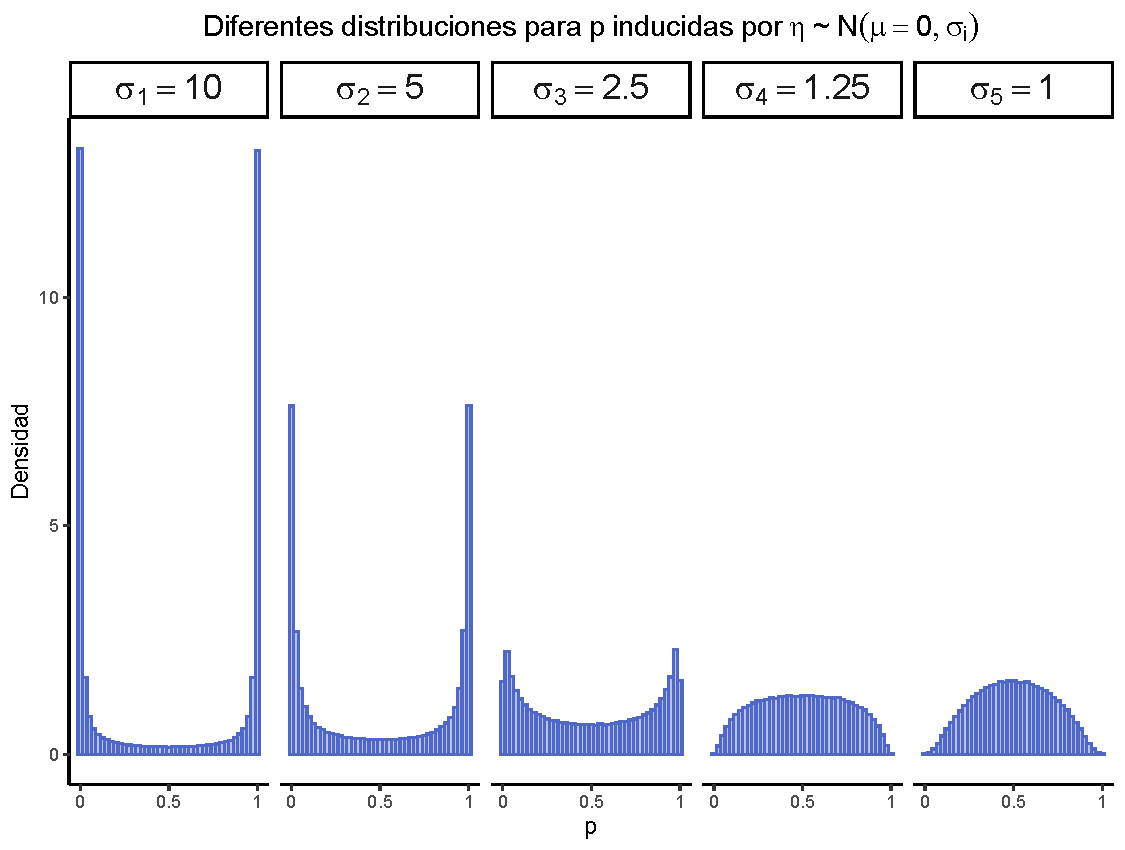
\includegraphics[width = 0.9\textwidth]{Figs/Modelado/Malas_Iniciales}
	\caption{Ejemplo de implicaciones en $p$ con distribuciones iniciales para un predictor lineal. Todas son normales centradas en $0$ con distintos parámetros $\sigma$ de desviación estándar. Fuente: elaboración propia.}
	\label{fig:Malas_Iniciales}
\end{figure}

El motivo es que la función logística no es lineal y tiene que ``compactar'' valores en los reales dentro del espacio confinado del $\left(0,1\right)$. Por decirlo de una manera informal, el verdadero rango de variación de la escala logística son valores de $\eta$ en $(-5,5)$; valores fuera de este intervalo llevan prácticamente a los mismos valores extremos cercanos a 0 o a 1, como apreciamos en la \textbf{Figura \ref{fig:Escala_Logis}}.\\

\begin{figure}[h]
	\centering
	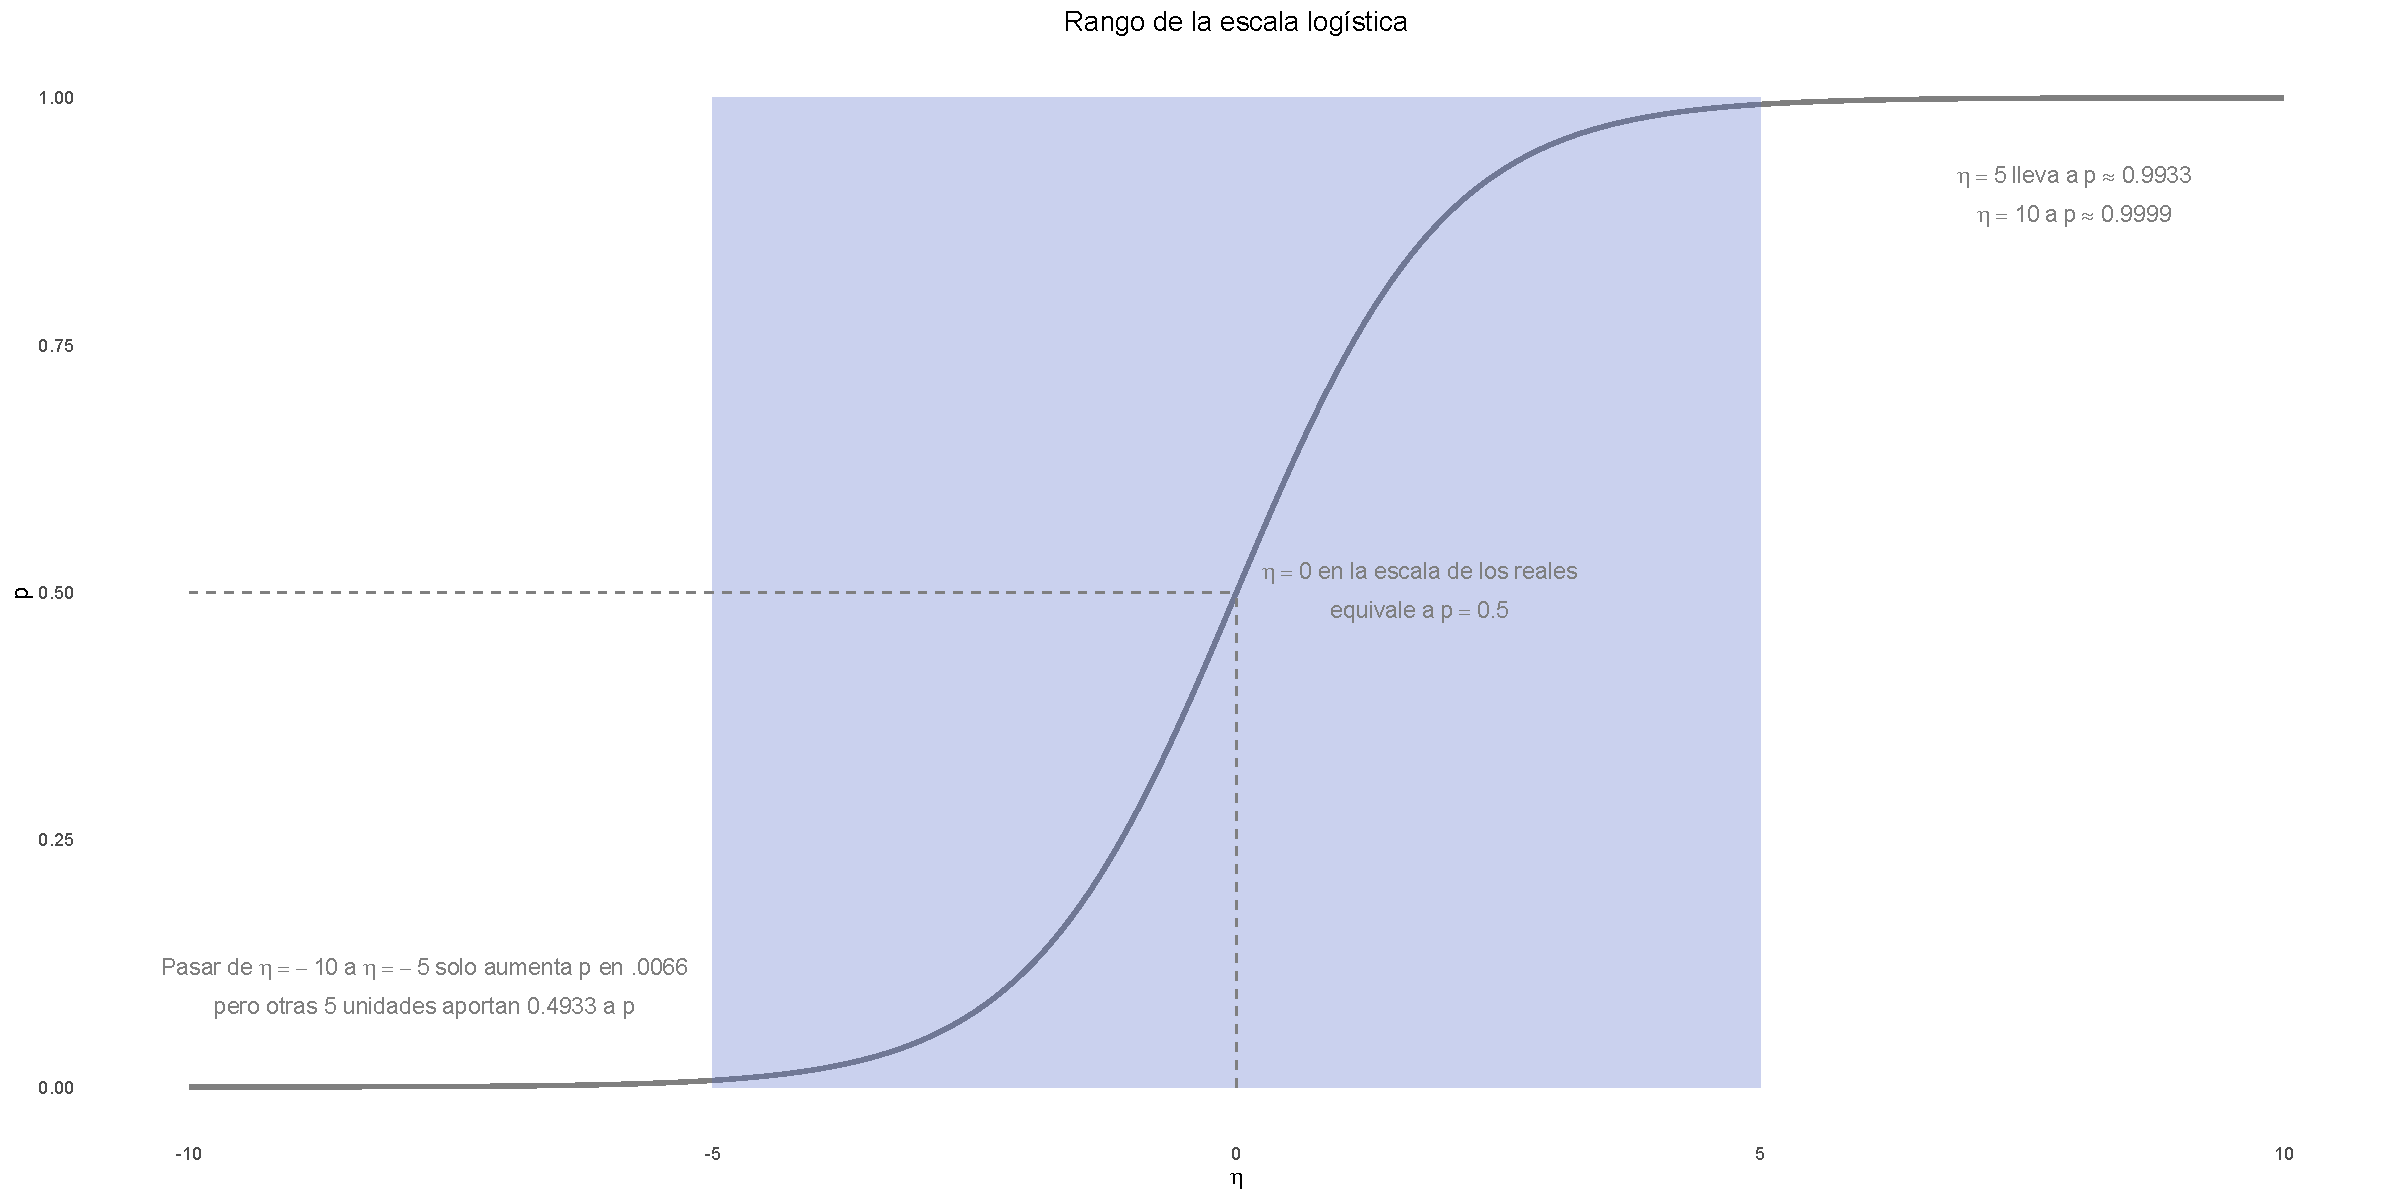
\includegraphics[width = 0.8\textwidth]{Figs/Modelado/Escala_Logis}
	\caption{Fuente: elaboración propia.}
	\label{fig:Escala_Logis}
\end{figure}

En este sentido, las distribuciones vagas con desviaciones estándar grandes permiten \textit{a priori} la existencia de efectos de una magnitud inverosímil, un problema análogo al que \textcite{Regueiro12} quiere evitar cuando discute el máximo número posible de goles en un partido de fútbol. Discusiones más detalladas sobre algunas posibles desventajas de utilizar distribuciones no informativas, sobre todo conforme aumenta la complejidad de los modelos considerados, pueden encontrarse en \textcites{PriorLikelihood17}{BetancourtStanShapePriors}{BlogSimpson}.\\

Ahora bien, no asignaré distribuciones iniciales para el predictor lineal en su conjunto, sino para los coeficientes de dicho predictor lineal, interpretados como efectos de variables explicativas sobre la variable de interés. No obstante, en lugar de optar por iniciales no informativas, propondré unas distribuciones más informativas aunque guiadas por una posición un poco escéptica. A pesar de lo que sugerían las tendencias ingenuas del capítulo anterior, \textit{a priori}, no buscaría asignarle un sentido al efecto. Asimismo, los efectos de variables ecológicas o agregadas, no deberían ser tan grandes, favoreciendo una desviación estándar más pequeña.\\ 

Considero que una inicial para un coeficiente $\beta\sim N(0,0.5^2)$ cumple relativamente bien con estas condiciones. Si tomamos el $0$ como referencia y comparamos el valor correspondiente de $p$ con aquel para una $\beta$ una desviación estándar mayor--- i.e. $\beta = 0.5$--- el efecto $\Delta$ sería de aproximadamente $+12$ puntos porcentuales. Si ahora disminuimos $\beta$ en 2 desviaciones estándar,  $\Delta \approx -23$ pp, como puede apreciarse en la \textbf{Figura \ref{fig:Inicial_Coef}}. Sin exagerar su interpretación, pues hay que multiplicar por el valor de la variable explicativa, estos podrían pensarse como los máximos efectos creíbles \textit{a priori}.\\ 

\begin{figure}[h]
	\centering
	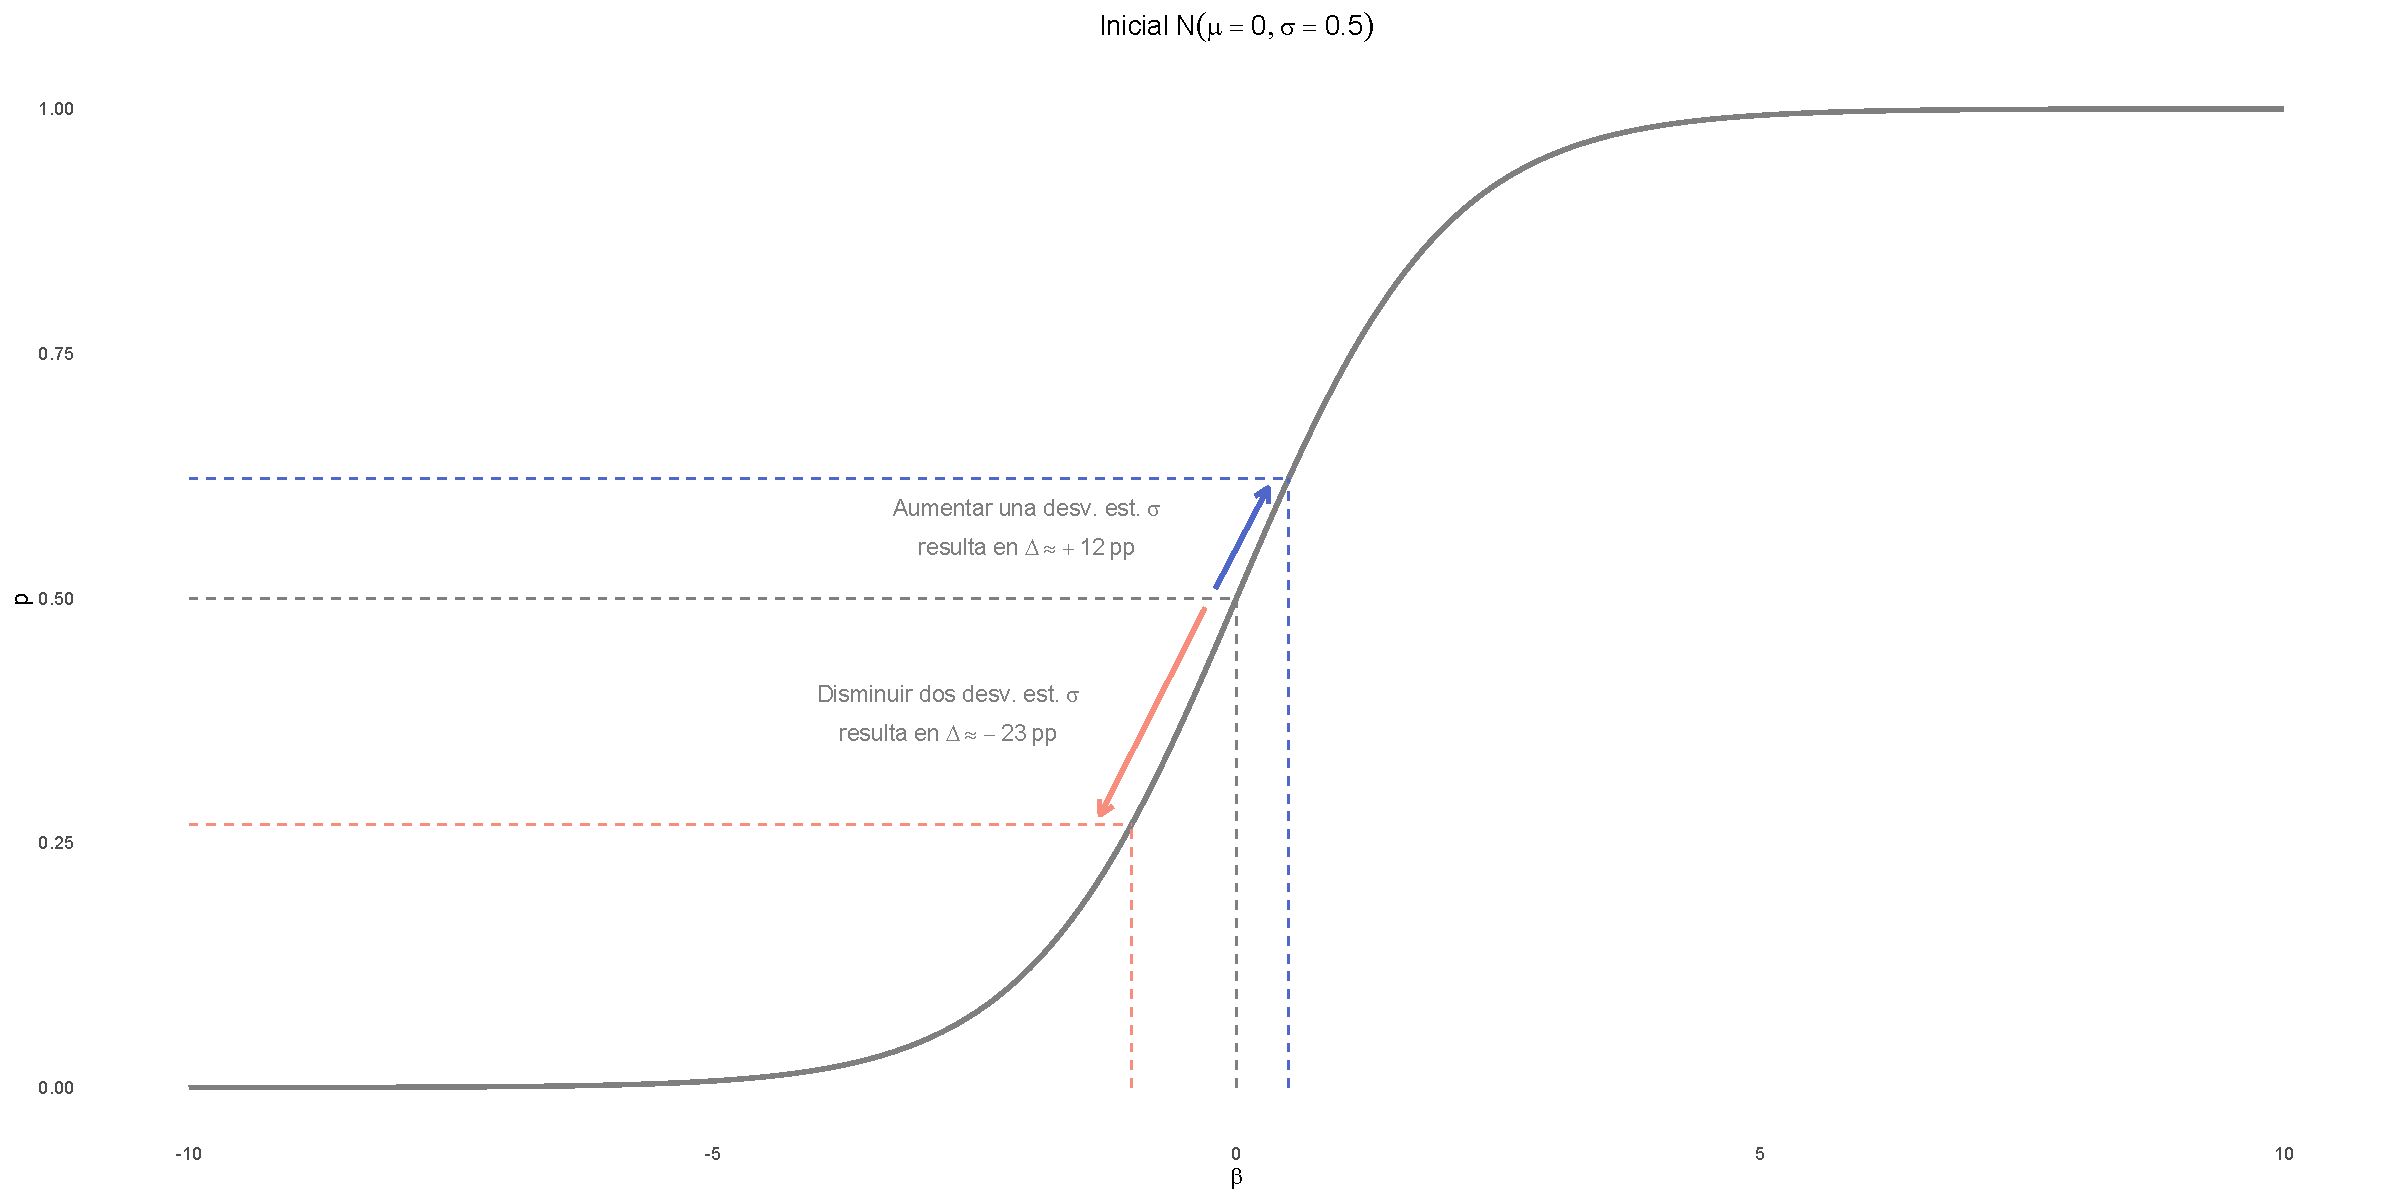
\includegraphics[width = 0.8\textwidth]{Figs/Modelado/Inicial_N0_un_medio}
	\caption{Fuente: elaboración propia.}
	\label{fig:Inicial_Coef}
\end{figure}

Por otro lado, debemos detenernos a pensar en la interpretación del intercepto $\alpha$. Por un lado, $\alpha$ es el valor que tomaría el predictor lineal $\eta_c$, si todos los coeficientes fueran iguales a $0$. Siguiendo las recomendaciones de pensar qué implicaciones tienen las distribuciones iniciales en las predictivas \parencite{BlogSimpson}, esto nos podría hacer pensar que querríamos que \textit{a priori} la inicial para $\alpha$ prediga valores cercanos al  17.46\%, porcentaje mediano de votos que obtuvo Le Pen en la elección. Sin embargo, también hay que notar que con variables explicativas de configuraciones sociales, $x_c$, $\alpha$ es el valor que tomaría $\eta_c$ si la población estuviera repartida equitativamente entre todas las categorías. En efecto, supongamos que para la $m$-ésima variable con $l_m$ categorías cada $x_{j,c}=l_m^{-1}$. Tendríamos que
\begin{align*}
\eta_c &= \alpha + \sum\limits_{j=1}^{l_m} \beta_j x_{j,c} = \alpha + \sum\limits_{j=1}^{l_m} \dfrac{\beta_j}{l_m} = \alpha + \dfrac{1}{l_m}\sum\limits_{j=1}^{l_m} \beta_j
\intertext{y por la restricción de identificabilidad de suma cero de los coeficientes,}
&= \alpha + \dfrac{1}{l_m}\left(0\right) = \alpha 
\end{align*}

Tomando en cuenta las teorías del conflicto discutidas en la revisión de literatura, podríamos pensar que si en lugar de tener grupos mayoritarios frente a grupos minoritarios hubiese una sociedad más ``equilibrada'', el voto frontista disminuiría. Así pues, deberíamos buscar una distribución inicial con una media menor al 17.5\%. También, considerando que puede ser más robusto dilucidar una distribución inicial con base en cuantiles, más que igualar la media podríamos intentar aproximar el rango intercuartílico observado de entre 13.54\% y 21.44\%, pero sesgado un poco a la baja para tomar en cuenta la hipótesis anterior sobre una población equilibrada. Después de algunas pruebas elegí una distribución inicial para $\alpha\sim N(-1.7,0.25^2)$.\\

Consideremos ahora una ``comuna promedio'', definida como aquella que tuviera valores promedio en las variables explicativas; podemos realizar simulaciones de la distribución predictiva con estas iniciales en su conjunto. Es decir, simulamos de $\alpha\sim N(-1.7,0.25^2)$ y para cada $\beta\sim N(0,0.5^2)$. Calculamos el predictor lineal con base en los valores promedio de cada categoría--- considerando también la restricción de suma cero de los coeficientes--- y tomamos el logit inverso. Este proceso, por ejemplo para grupos de edad, nos lleva al histograma de la \textbf{Figura \ref{fig:Predictiva_Inicial}}, con el modelo
\begin{align*}
y_c|\theta=(\alpha,\beta) & \sim Binom(n_c,p_c) \quad \forall \quad c \in \mathbb{N}_C \\
\text{con} \quad log\left(\dfrac{p_c}{1-p_c}\right) &= \alpha + \beta_1 x_{edad,1,c} + \dots + \beta_6 x_{edad,6,c} \quad \text{tal que} \quad \sum\limits_{j = 1}^6 \beta_j = 0 \nonumber \\
\text{y} \quad \alpha & \sim N(-1.7,0.25^2)\\
\beta_j & \sim N(0,0.5^2) \quad \, j \in \mathbb{N}_{5} 
\end{align*}

\begin{figure}[h]
	\centering
	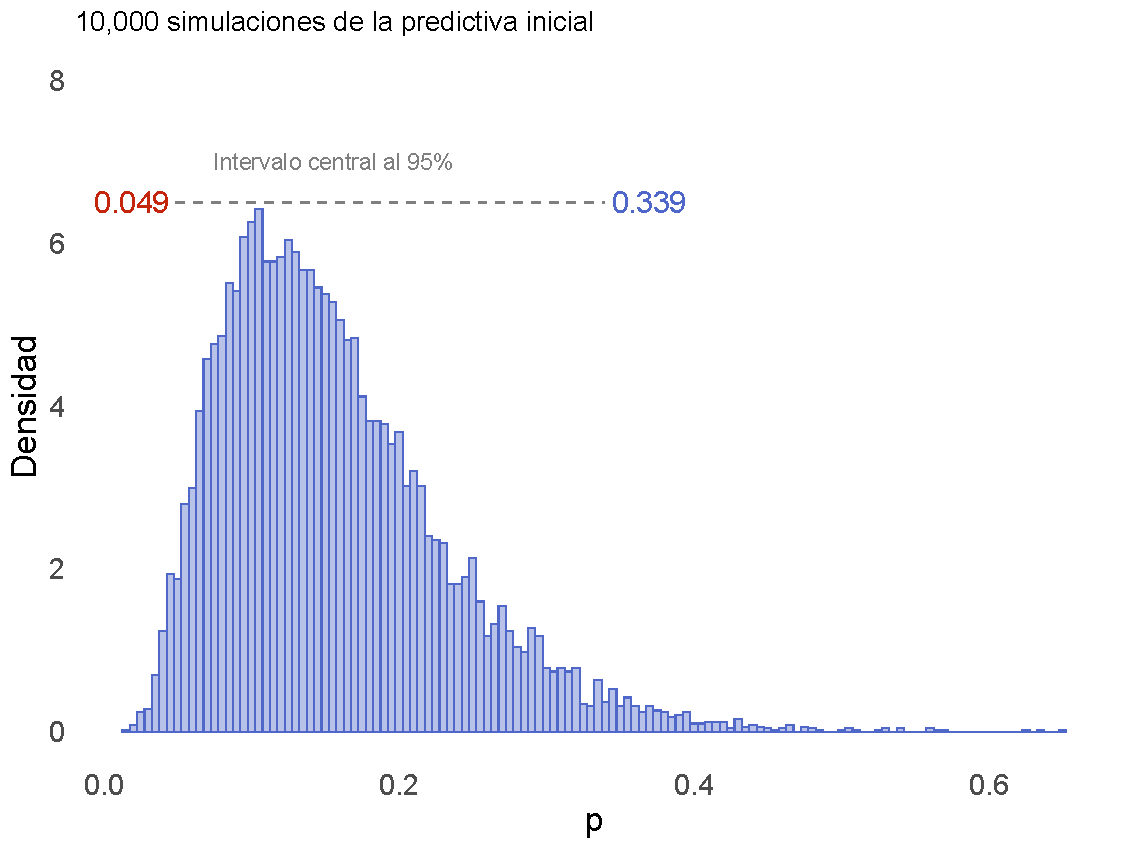
\includegraphics[width = 0.8\textwidth]{Figs/Modelado/Pred_Inicial}
	\caption{Fuente: elaboración propia.}
	\label{fig:Predictiva_Inicial}
\end{figure}

Estas distribuciones iniciales, como ya he mencionado, son subjetivas y podrían considerarse como informativas. Algún lector podría no estar muy convencido de la elección que realizo, por lo que eran importantes los párrafos anteriores de manera que fuera más transparente el proceso por el cual llegué a elegirlas. Adicionalmente, después de presentar los modelos considerados hasta culminar con un modelo final, describiré un pequeño análisis de sensibilidad que contribuye a la justificación de estas distribuciones iniciales.\\  

\section{Modelos individuales}

Consideremos entonces, para la $m$-ésima variable censal con $l_m$ categorías poblacionales, modelos de la siguiente forma:
\begin{align}\label{eq:Modelo_Nal_Ind}
y_c|\theta=(\alpha,\beta) & \sim Binom(n_c,p_c) \quad \forall \quad c \in \mathbb{N}_C \nonumber \\
\text{con} \quad log\left(\dfrac{p_c}{1-p_c}\right) &= \alpha + \sum\limits_{j=1}^{l_m} \beta_j x_{m,j,c} \quad \text{tal que} \quad \sum\limits_{j = 1}^{l_m} \beta_j = 0 \nonumber \\
\text{y} \quad \alpha & \sim N(-1.7,0.25^2) \nonumber \\
\beta_j & \sim N(0,0.5^2) \quad \, j \in \mathbb{N}_{l_m-1} 
\end{align}

A \eqref{eq:Modelo_Nal_Ind} le llamaré un \textbf{Modelo Nacional Individual} porque se tienen coeficientes a nivel nacional\footnote{En realidad, como mencionaba en el análisis exploratorio de datos, son coeficientes para la metrópoli y no para todo el país.} y solo incluyo una variable explicativa de manera individual. Tendría entonces 9 modelos nacionales individuales de esta forma. Sin embargo, el análisis exploratorio de datos sugería que se podría modelar de mejor manera dejando que los coeficientes e interceptos variasen para cada uno de los 96 departamentos. Es decir, podríamos construir igualmente 9 \textbf{Modelos Jerárquicos Individuales}. Si denotamos como $d[c]$ el \textit{departamento} al que pertenece la comuna $c$, el $m$-ésimo modelo jerárquico individual sería: 
\begin{align}\label{eq:Modelo_Jer_Ind}
y_c|\theta & \sim Binom(n_c,p_c) \quad \forall \, c \in \mathbb{N}_C \nonumber \\
\text{con} \quad log\left(\dfrac{p_c}{1-p_c}\right) &= \alpha_{d[c]} + \sum\limits_{j=1}^{l_m} \beta_{d[c],j} x_{m,j,c} \nonumber\\ 
\text{tal que} \quad -\sum\limits_{j = 1}^{l_m} \beta_{d,j} = 0 \nonumber \\
\alpha_d & \sim N(\mu_{\alpha}, 1) \quad \forall \, d \in \mathbb{N}_{96} \nonumber \\
\beta_{d,j} & \sim N(\mu_{\beta}, 1) \quad \forall \, j \in \mathbb{N}_{l_m-1}  \quad \text{y} \quad d \in \mathbb{N}_{96} \nonumber \\
\mu_{\alpha} &\sim N(-1.7, 0.25^2) \nonumber \\
\mu_{\beta} &\sim N(0,0.5^2)
\end{align}

Se corrieron cada uno de los 18 modelos individuales mediante el software Stan, simulando vía \textit{Hamiltonian Monte Carlo} las distribuciones posteriores dada la muestra de datos discutida en la \textbf{\autoref{secc:muestra}}. Una vez con dichas distribuciones posteriores, podemos hacer lo que \textcite{Gelman13} llaman \textit{posterior predictive checks}. Podemos predecir el porcentaje esperado de votos en cada una de las comunas y calcular su error respecto al real. Para el modelo nacional de ocupación laboral juvenil, los resultados están en la \textbf{Figura \ref{fig:Modelo_Nal_Ocu_Juvenil}}.\\

\begin{figure}[h]
	\centering
	\includegraphics[width = 0.8\textwidth]{Figs/Modelado/Modelo_Nal_Ocu_Juvenil}
	\caption{Mapa de predicciones medias del porcentaje bruto de votos obtenido por Marine Le Pen en las presidenciales 2012 mediante el Modelo Nacional por Ocupación Juvenil (izq.) y mapa de los respectivos errores (der.). Fuente: elaboración propia con la cartografía de Open Street Map.}
	\label{fig:Modelo_Nal_Ocu_Juvenil}
\end{figure}

En el mapa de la izquierda las predicciones se colorean de acuerdo a la escala real que va de 0\% a 62.5\% y donde el cambio de tonos rojos a azules se da en la comuna mediana de 17.5\%. Observamos que la predicción en general subestima el verdadero porcentaje obtenido pues el mapa está prácticamente coloreado en su totalidad de tonos rojos. Sin embargo, las predicciones están cerca de la mediana. De hecho, el mapa de errores--- verde significa poco error y naranjas y rojos más--- visualmente es prácticamente un negativo del verdadero mapa de resultados que observábamos en la \textbf{Figura \ref{fig:Mapa_Pct_Br}} del capítulo anterior.\\

En general, los modelos nacionales tienen el defecto de no reconocer la enorme variabilidad geográfica del fenómeno electoral. Si construimos distintas medidas de error de predicción vemos que pasar de un modelado nacional a un modelado jerárquico las reduce consistentemente. Para cada simulación posterior predecimos el número de votos en cada comuna, departamento y a nivel nacional. Luego lo convertimos en porcentaje bruto de votos predicho dividiendo entre el número de inscritos. Así, podemos tomar los conocidos errores absoluto y cuadrático promedio para el porcentaje de votos a nivel comuna, departamento y nacional. Incluso podemos tomar una pérdida más arbitraria, pero ilustrativa, como el porcentaje promedio de estimaciones que se encuentran a más de 1.5 puntos porcentuales del verdadero valor en los 3 niveles de agregación; a esta medida la llamo tolerancia 1.5 pp. Finalmente se calcula el promedio de las medidas a través del total de simulaciones posteriores y se grafican en la \textbf{Figura \ref{fig:Errores_Modelos_Individuales}}. El gráfico también incluye el cálculo de un cuarto error para las comunas llamado WAIC, pero a él me refiriré más adelante. En el gráfico, los puntos son las medidas para el modelo nacional y las flechas las de los modelos jerárquicos.\\ 

\begin{figure}[h]
	\centering
	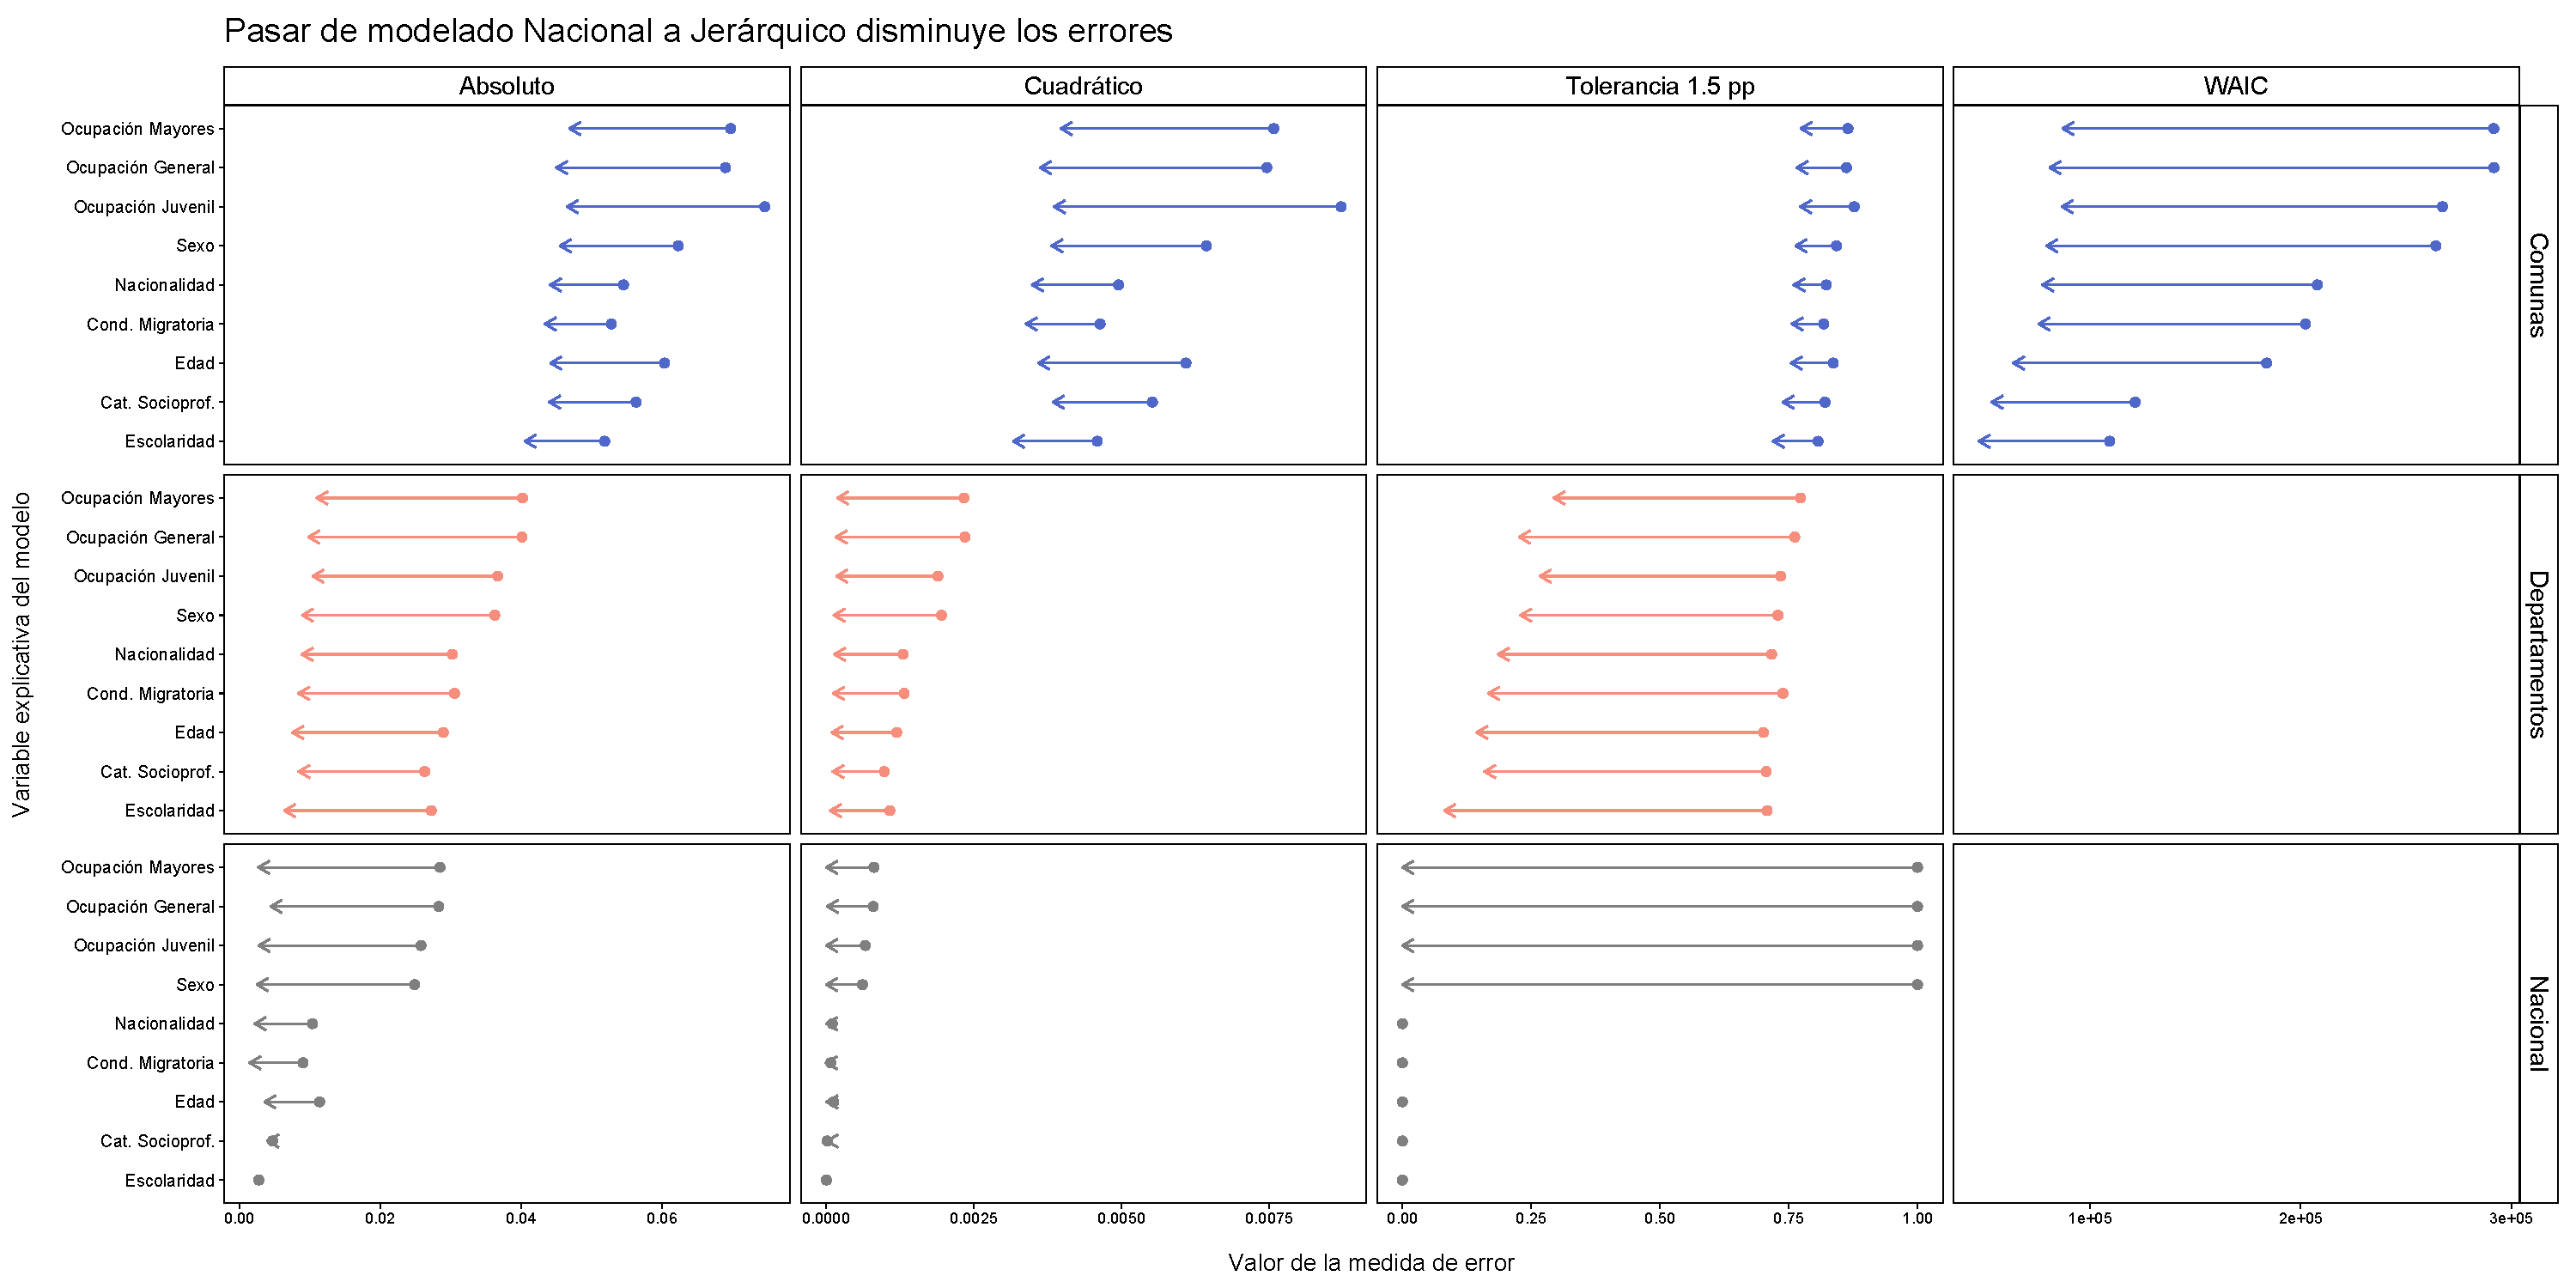
\includegraphics[width = 0.8\textwidth]{Figs/Modelado/Graf_Errores_Modelos_Individuales}
	\caption{Comparación de los modelos nacionales y jerárquicos individuales bajo diferentes medidas de error. Fuente: elaboración propia.}
	\label{fig:Errores_Modelos_Individuales}
\end{figure} 

Como es de esperarse, los modelos estiman de mejor manera los porcentajes de niveles de mayor agregación que el del nivel comunal. Viendo la pérdida arbitraria llamada de tolerancia 1.5, salvo las variables de sexo y ocupaciones, todas las predicciones estiman un porcentaje de votos nacional a menos de 1.5 puntos porcentuales del real. Sin embargo, vemos que los modelos nacionales solo logran esta precisión de estimación en alrededor de 70 de los 96 departamentos.\\ 

Esto refleja lo que había mencionado al ver el mapa de predicciones para el modelo nacional individual por ocupación juvenil. Al no permitir que los coeficientes varíen por departamento, el modelo ajusta para el país entero, sacrificando las estimaciones en las diferentes zonas geográficas que estos constituyen. Si observamos medidas de error más tradicionales como la absoluta o la cuadrática vemos que todas las flechas se dirigen a la izquierda, es decir que se reducen los errores al reconocer esa variabilidad geográfica. Ahora bien, estas 3 medidas tienen más un carácter ilustrativo y sirven para recordar que se pueden construir diferentes errores para diferentes estimadores.\\ 

Ahora notemos que las variables de solo 2 categorías como ocupación, sexo, nacionalidad y condición migratoria tienen peor desempeño que las de más categorías como edad, categoría socioprofesional y escolaridad. ¿Esto quiere decir que son peores variables explicativas? ¿No podría esto deberse a que las últimas tienen más parámetros y es más fácil ajustar mejor simplemente por introducir parámetros adicionales?\\

\subsection{WAIC}

Pensando en la posibilidad de mejorar un ajuste simplemente haciendo más complejo el modelo es que una mejor y más aceptada medida de error es el llamado WAIC por sus siglas en inglés \textit{Widely Applicable} o \textit{Watanabe-Akaike Information Criterion} \parencite{Vehtari16}. El WAIC busca estimar la capacidad predictiva de un modelo via las predictivas posteriores de los datos con los que se ajusta. La intuición es que a mayor valor de la predictiva posterior para el dato observado, mayor la posibilidad de predecir otros datos.\\ 

Para un conjunto de $n$ datos $y=(y_1,\dots,y_n)$ y una muestra posterior de parámetros $\left\lbrace\theta_{(s)}\right\rbrace_{s=1}^S$, el WAIC se define de la siguiente manera:
\begin{align}\label{WAIC}
WAIC(y|\theta) &= \widehat{lpd} + \widehat{par} \\
\text{con} \quad \widehat{lpd} &= \sum_{i=1}^{n} log\left(\dfrac{1}{S}\sum\limits_{s=1}^S f(y_i|\theta_{(s)}) \right) \nonumber \\
\text{y} \quad \widehat{par} &= \sum\limits_{i=1}^n V(y_i|\theta), \nonumber
\end{align}

donde $V(y_i|\theta)=\dfrac{1}{S-1}\sum\limits_{s=1}^S \mathcal{L}(y_i;\theta_{s})^2$ y $\mathcal{L}(y_i;\theta_{s}) = log\left[f(y_i|\theta_{(s)})\right] - \dfrac{1}{S}\sum\limits_{s=1}^S log\left[f(y_i|\theta_{(s)})\right]$.{}\\

El WAIC se conforma de dos sumas. La primera, $\widehat{lpd}$, es una aproximación de la log predictiva posterior, es decir una medidad de ajuste. Por otro lado, $\widehat{par}$ es normalmente llamado el \textit{número efectivo estimado de parámetros} y, mediante sumas de varianzas, busca medir la complejidad del modelo. En total, entre menor sea el valor del WAIC, esperaríamos un mejor desempeño predictivo tomando en cuenta la complejidad del modelo.\\

Así pues, observando los valores del WAIC para cada modelo (\textbf{Figura \ref{fig:Errores_Modelos_Individuales}}), podríamos comenzar a pensar que efectivamente hay un ordenamiento en el poder predictivo de las distintas variables: escolaridad, categorías socioprofesionales, edad, condición migratoria, nacionalidad, sexo y, finalmente, las ocupaciones. Sin concluir todavía nada, parecería que a las hipótesis sobre inseguridad laboral no les corresponde el mejor de los poderes explicativos en términos de estos modelos.\\

\section{Modelos compuestos}

Este ordenamiento preliminar tiene el objetivo de ayudarme a construir, secuencialmente, un modelo cada vez más complejo. Para comenzar, veamos los mapas de predicción que generó el modelo con menor WAIC, el jerárquico por escolaridad, en la \textbf{Figura \ref{fig:Modelo_Jer_Escolaridad}}.\\ 

\begin{figure}[h]
	\centering
	\includegraphics[width = 0.8\textwidth]{Figs/Modelado/Modelo_Jer_Escolaridad}
	\caption{Mapa de predicciones medias del porcentaje bruto de votos obtenido por Marine Le Pen en las presidenciales 2012 mediante el Modelo Jerárquico por Escolaridad (izq.) y mapa de los respectivos errores (der.). Fuente: elaboración propia.}
	\label{fig:Modelo_Jer_Escolaridad}
\end{figure}

El mapa de errores ya se observa más verde y homogéneo. Las grandes zonas de fortaleza y debilidad del FN comienzan a ser identificadas por el modelo. Sin embargo, los tonos de algunas predicciones son todavía demasiado cercanos a la mediana. En el centro observamos una zona de tonos muy claros, casi blancos, que no corresponden totalmente a la realidad. En general, vemos que hay menor variabilidad dentro de los departamentos de la que se observó en la elección.\\ 

Estas reflexiones sugieren que, en lugar de tomar una a una las variables, podemos ir agregando variables a la regresión en modelos jerárquicos secuenciales que refinen el ajuste. Entonces, este modelo jerárquico por escolaridad podríamos considerarlo el \textbf{Modelo 0}, pues partiremos de él para ir agrandándolo con la inclusión de una nueva variable cada vez.\\ 

El primer modelo compuesto incluye las variables de escolaridad y categorías socioprofesionales. A este modelo lo llamaré el \textbf{Modelo A}. Para distinguir las variables utilizaré diferentes letras griegas para sus coeficientes. Para la configuración social de escolaridad 
\[x_{escol,c} = (Esc_c,Dip1_c,Dip2_c,Dip3_c,Dip4_c)^T\]
en la comuna $c$ los coeficientes departamentales serán un vector $\beta_{d[c]} = (\beta_{d[c],1},\dots,\beta_{d[c],5})$. Para las categorías socioprofesionales $x_{csp,c}$ los coeficientes serán $\gamma_{d[c]}$:
\begin{align}\label{eq:Modelo_Comp_A}
y_c|\theta & \sim Binom(n_c,p_c) \quad \forall \, c \in \mathbb{N}_C \nonumber \\
\text{con} \quad ln\left(\dfrac{p_c}{1-p_c}\right) &= \alpha_{d[c]} + \beta_{d[c]} x_{escol,c} + \gamma_{d[c]} x_{csp,c} \\ 
\intertext{tal que} 
\sum\limits_{j = 1}^{5} \beta_{d,j}=0, \quad & \sum\limits_{j = 1}^{8} \gamma_{d,j}=0, \nonumber \\
\alpha_d & \sim N(\mu_{\alpha}, 1), \nonumber \\
\intertext{donde $\forall \, d \in \mathbb{N}_{96}$}
\beta_{d,j} \sim N(\mu_{\beta}, 1) \quad \forall \, j \in \mathbb{N}_{4}, & \quad \gamma_{d,j} \sim N(\mu_{\gamma}, 1) \quad \forall \, j \in \mathbb{N}_{7} \nonumber \\
\intertext{y}
\mu_{\alpha} \sim N(-1.7, 0.25^2), \quad \mu_{\beta} &\sim N(0, 0.5^2) \quad \text{y} \quad \mu_{\gamma} \sim N(0,0.5^2). \nonumber
\end{align}

Al estimar el modelo con ambas variables el WAIC mejora. Asimismo, observando los mapas de la \textbf{Figura \ref{fig:Modelo_Compuesto_A}}, vemos que se reduce la gran zona blanquiza del centro, se comienza a observar mayor variabilidad dentro de los departamentos y los tonos también se oscurecen más, sobre todo en el noreste.\\ 

\begin{figure}[h]
	\centering
	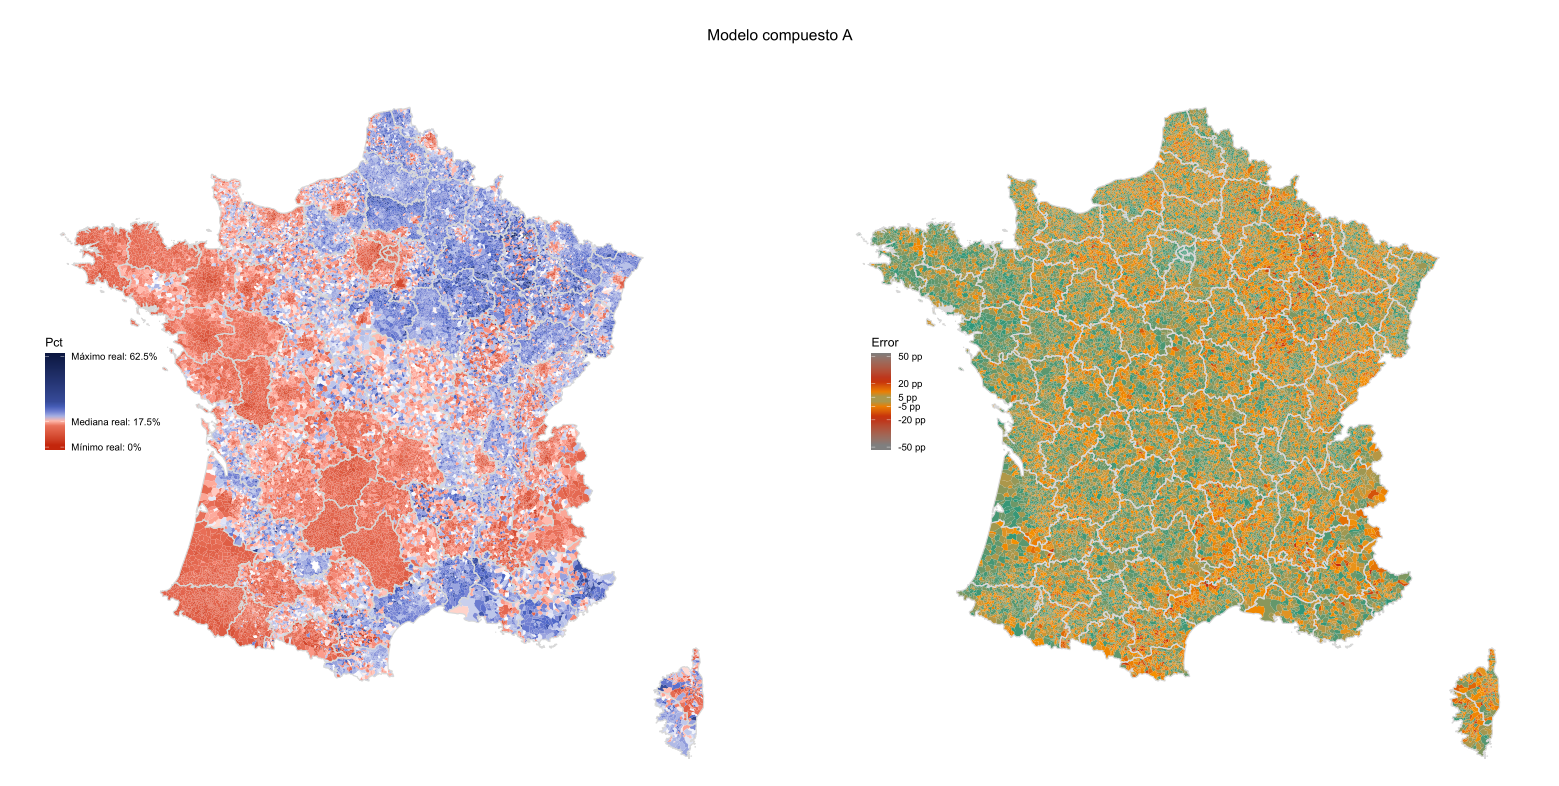
\includegraphics[width = 0.8\textwidth]{Figs/Modelado/Modelo_Compuesto_A}
	\caption{Mapas de predicciones medias (izq.) y respectivos errores (der.) para el porcentaje bruto de votos obtenido por Marine Le Pen en las presidenciales 2012 mediante el Modelo Jerárquico por Escolaridad y Categorías socioprofesionales. Fuente: elaboración propia.}
	\label{fig:Modelo_Compuesto_A}
\end{figure}

Los siguientes modelos se llamarán de manera progresiva por letras latinas y sus planteamientos en términos de ecuaciones pueden encontrarse en el \textbf{\autoref{Anexo_modelos_compuestos}}. Por ejemplo, el \textbf{Modelo B} incorpora los grupos de edad $x_{edad,c}$. Debido a la similitud entre condición migratoria y nacionalidad, solamente buscaba incorporar una de las dos, tratando de identificar la que tuviera mejor desempeño. De acuerdo al ordenamiento previo en los modelos individuales, consideraré solo la variable migratoria $x_{migr,c}$ dentro del \textbf{Modelo C}. Por su parte, el \textbf{Modelo D} incluye la distribución comunal por sexo $x_{sexo,c}$.\\

Después comenzaríamos a incluir las variables de ocupación. Como mencionaba al presentarlas, tengo un interés especial en la (des)ocupación juvenil, pues esta sería una variable que referencias como \textcite{LeBras16} y \textcite{Perrineau07} favorecerían. Por ello, al margen del ordenamiento, construí dos modelos de 6 variables. De manera general ambos incorporan una variable explicativa $x_{ocu,c}$. El \textbf{Modelo E} es el modelo D más la ocupación juvenil, mientras que el \textbf{Modelo F} es el modelo D más la ocupación general. Una vez generados por separado, podemos considerar un modelo que incorpore ambas variables, este sería el \textbf{Modelo G}. Finalmente agregamos la última variable considerada, la ocupación para personas de 55 a 64 años $x_{ocu\_may,c}$, para obtener el \textbf{Modelo H}, cuyos mapas corresponden a la \textbf{Figura \ref{fig:Modelo_Compuesto_H}}.\\

\begin{figure}[h]
	\centering
	\includegraphics[width = 0.8\textwidth]{Figs/Modelado/Modelo_Compuesto_H}
	\caption{Mapas de predicciones medias (izq.) y respectivos errores (der.) para el porcentaje bruto de votos obtenido por Marine Le Pen en las presidenciales 2012 mediante el Modelo Jerárquico por Escolaridad, Categorías socioprofesionales, Edad, Condición migratoria, Sexo y Ocupaciones. Fuente: elaboración propia.}
	\label{fig:Modelo_Compuesto_H}
\end{figure}

¿Cuál es la comparación de WAICs entre todos estos modelos? En la \textbf{Figura \ref{fig:Compara_WAIC_Compuestos}} podemos observarlo. En general, el WAIC mejora conforme se van agregando variables. Ciertamente las mayores ganancias se dan al agregar las primeras variables que el análisis individual sugería eran las más explicativas. Esto parece reforzar dicha hipótesis. Por el contrario, en términos de WAIC, la ocupación juvenil no parece ser la más poderosa de las variables. En efecto, la ganancia en WAIC frente al modelo D al agregarla en el modelo E es de apenas 46 unidades, menor a la ganancia del modelo F que fue de 162. Más aún, al pasar del modelo F al modelo G agregándola de nuevo, la ganancia vuelve a ser poca, apenas de 29. Esto no quiere decir, sin embargo, que no aporte nada a la regresión. Aunque la mejora en WAIC sea pequeña esta es positiva por lo que tenemos mejores modelos al incluirla.\\

\begin{figure}[h]
	\centering
	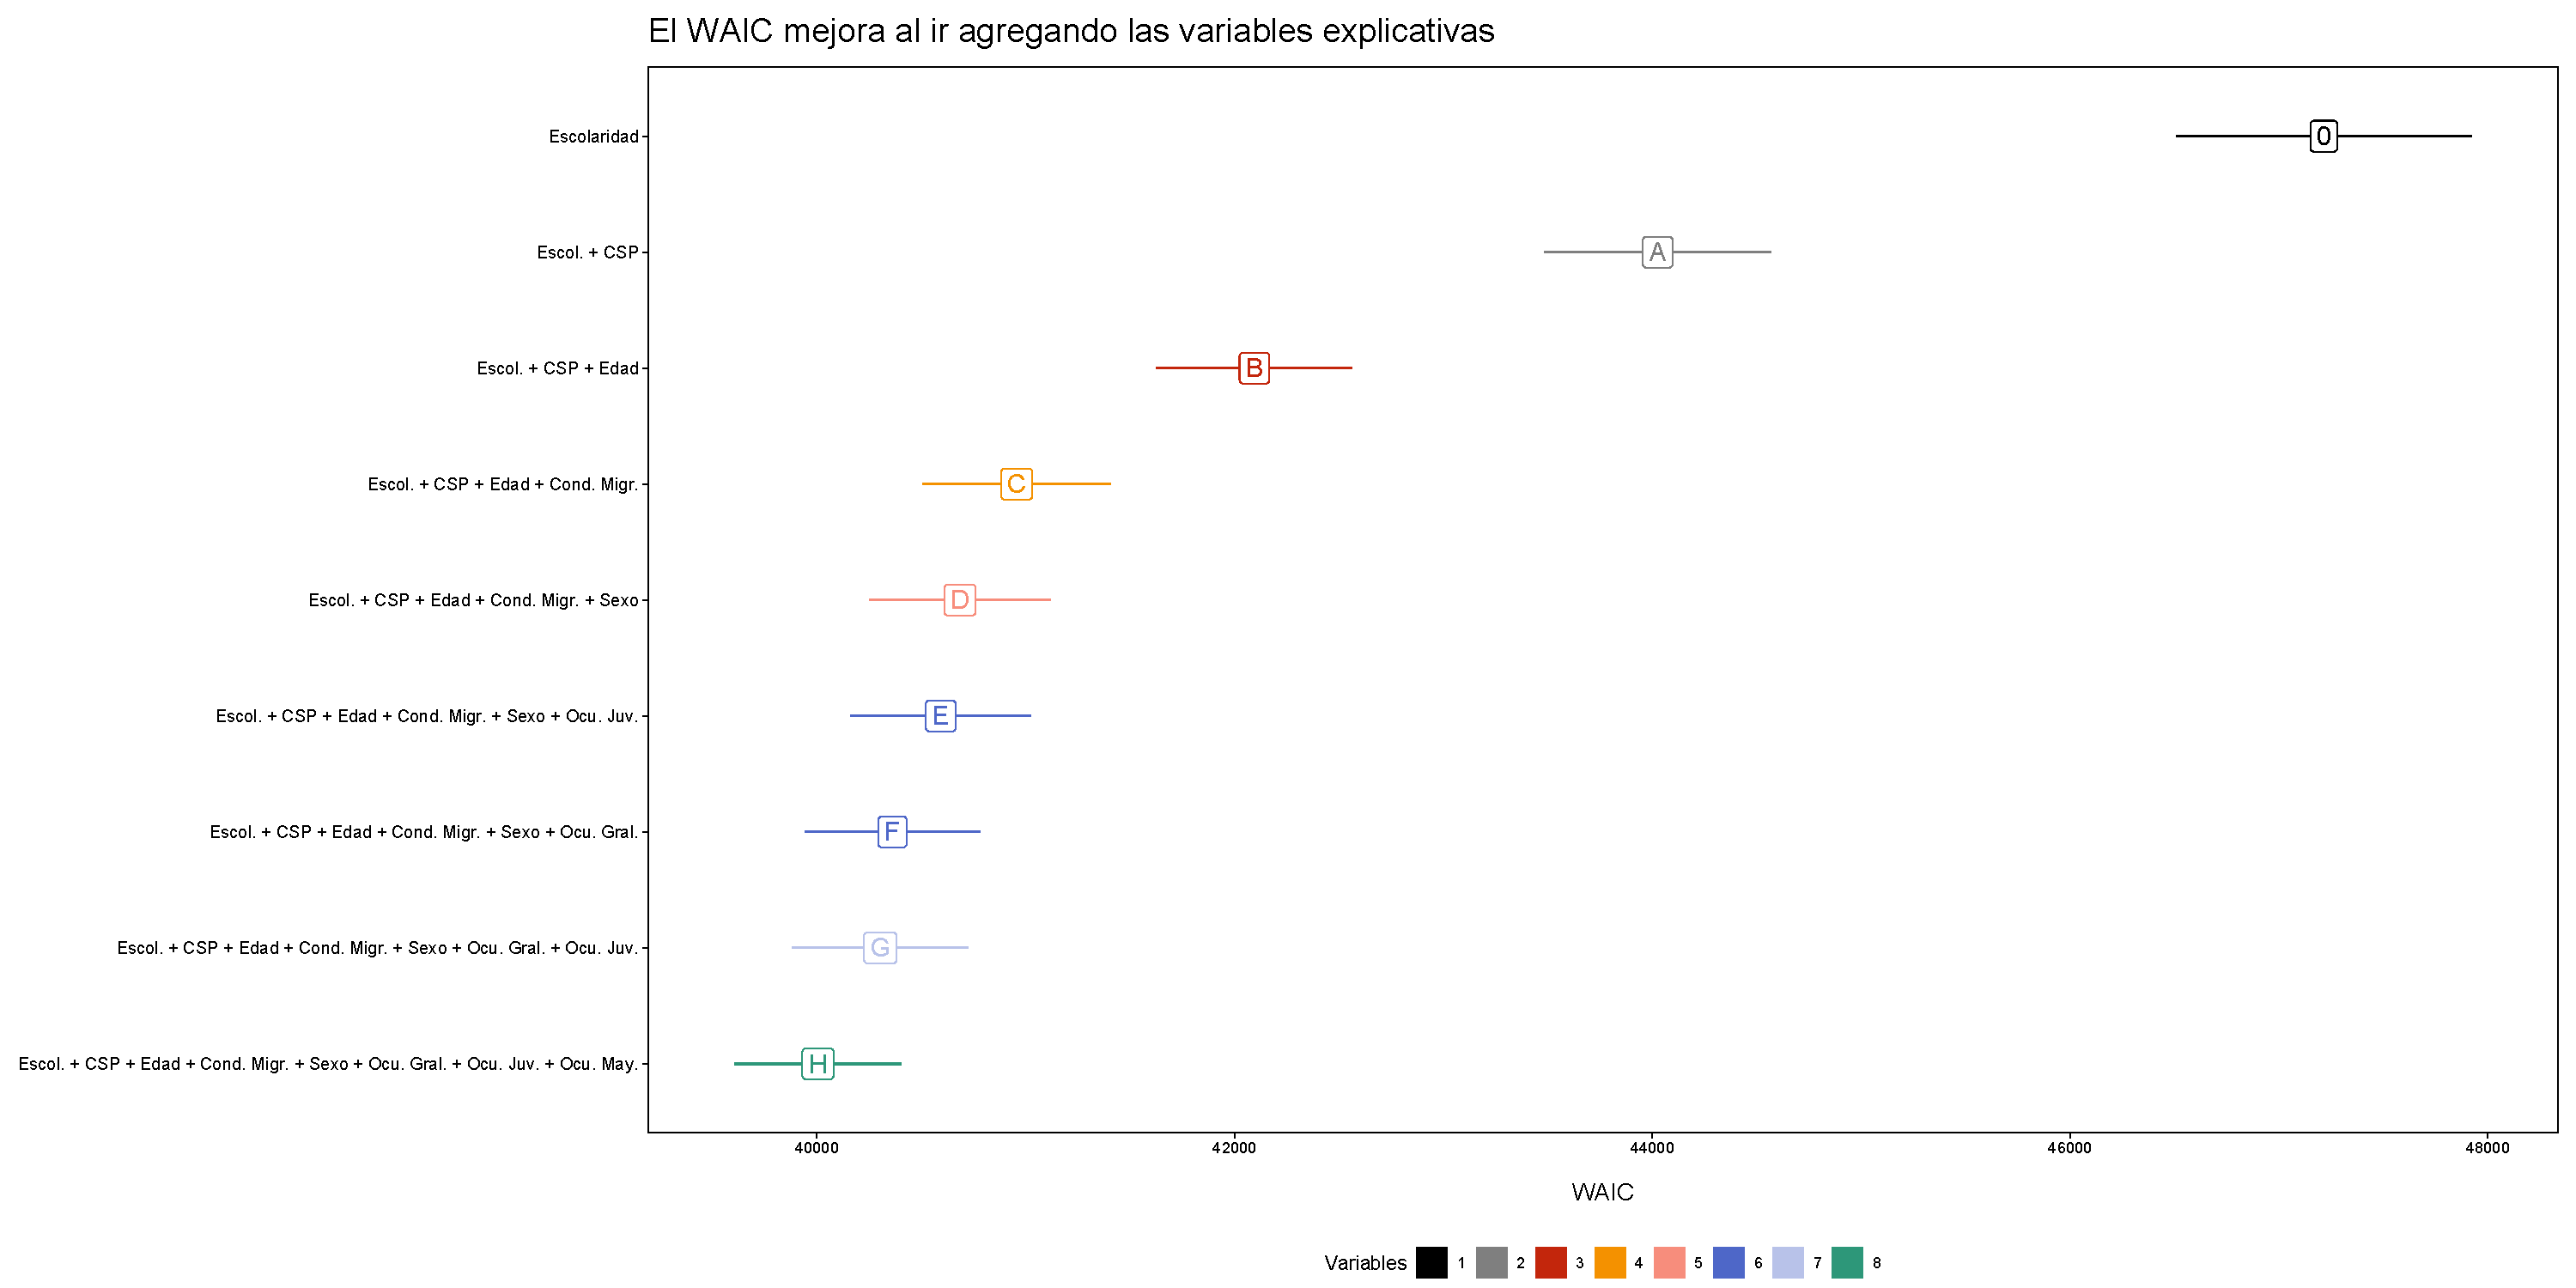
\includegraphics[width = 0.9\textwidth]{Figs/Modelado/Graf_WAIC_Modelos_Compuestos}
	\caption{Comparativo de WAIC para distintos modelos. Comenzando por el modelo 0 que incluye solo escolaridad se van añadiendo variables hasta incluirlas todas en el modelo H. Fuente: elaboración propia.}
	\label{fig:Compara_WAIC_Compuestos}
\end{figure}

El mejor modelo en términos de WAIC es el modelo H, por lo que será este el que interpretaré. Sin embargo, antes de ello, como adelantaba en la \autoref{sec:Convergencia}, hay que verificar que las cadenas simuladas mediante la implementación de HMC dentro de Stan hubieran convergido. En esta discusión de convergencia también menciono un pequeño análisis de sensibilidad respecto a la elección de distribuciones iniciales informativas.\\

\subsection{Convergencia de HMC}

Debido a la cantidad de parámetros dentro de cada modelo, así como a la cantidad de modelos ajustados en sí, es difícil verificar a detalle todas y cada una de las muestras posteriores. Afortunadamente, \textcite{BetancourtRStanWorkflow} desarrolla un caso de estudio en el que ilustra cómo programar distintos diagnósticos útiles para todos los parámetros de interés dentro de todos los modelos. Entre ellos encontramos el factor de reducción de escala $\hat{R}$, así como un cálculo del tamaño efectivo de muestra por iteración y 3 diagnósticos particulares de HMC. Utilizando su código abierto\footnote{Los derechos de autor son de Michael Betancourt y la Universidad de Columbia y las licencias específicas pueden verificarse en el link en las referencias.}, verificamos que los modelos satisfacen los criterios planteados y podemos confiar en la convergencia de las muestras posteriores obtenidas. Esta comprobación puede reproducirse con el código del repositorio de Github de esta tesis y solicitándome acceso a los archivos .rds con los ajustes de todos los modelos.\\

 Adicionalmente, podemos observar algunos diagnósticos gráficos para algunos parámetros del modelo H. Por ejemplo, en la \textbf{Figura \ref{fig:Traceplots_H}} observamos en los \textit{traceplots} que hay una buena mezcla de las cadenas; esto también se confirma viendo que las densidades por cadena de la \textbf{Figura \ref{fig:Densidades_H}} son parecidas. Finalmente, en la \textbf{Figura \ref{fig:Autocorr_H}} vemos que las autocorrelaciones son pequeñas. De hecho, existe un poco de simulación antitética que permite una mejor eficiencia en el tamaño de muestra \parencite{BlogAntithetical}.\\ 
 
 \begin{figure}[h]
	\centering
	\begin{subfigure}{0.45\textwidth}
	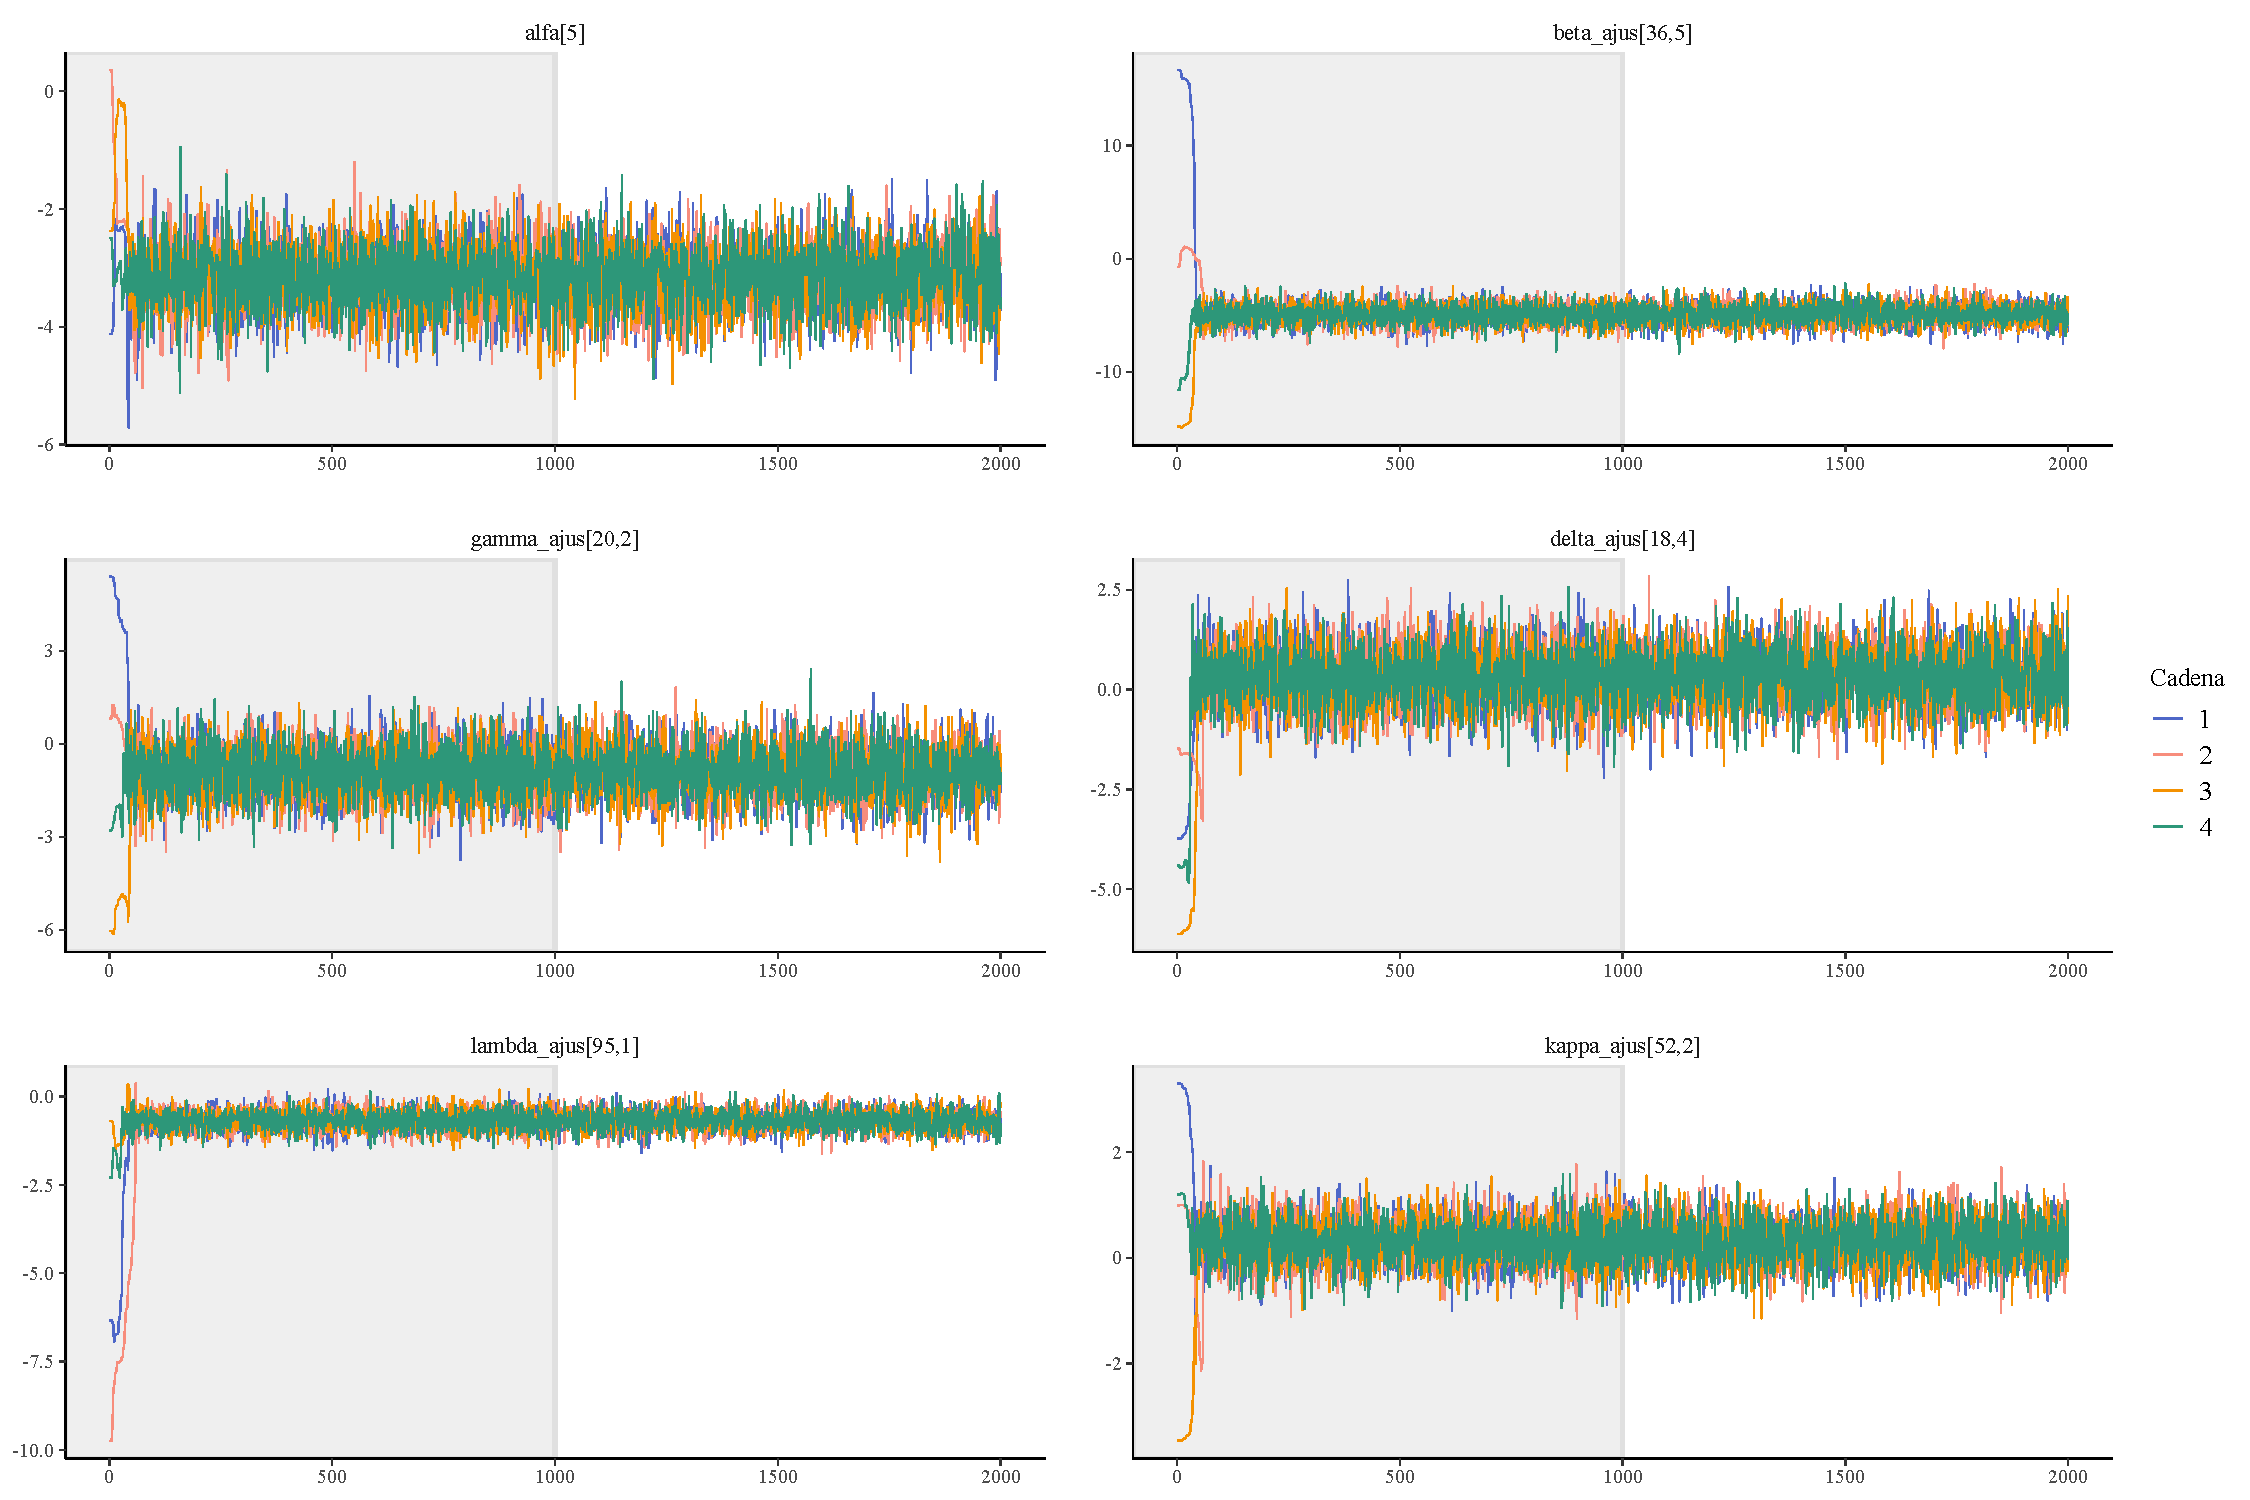
\includegraphics[width = \textwidth]{Figs/Convergencia/Convergencia_Traceplots}
	\caption{Ejemplo de \textit{traceplots} para algunos parámetros del modelo H.}
	\label{fig:Traceplots_H}
	\end{subfigure}
	~
	\begin{subfigure}{0.45\textwidth}
	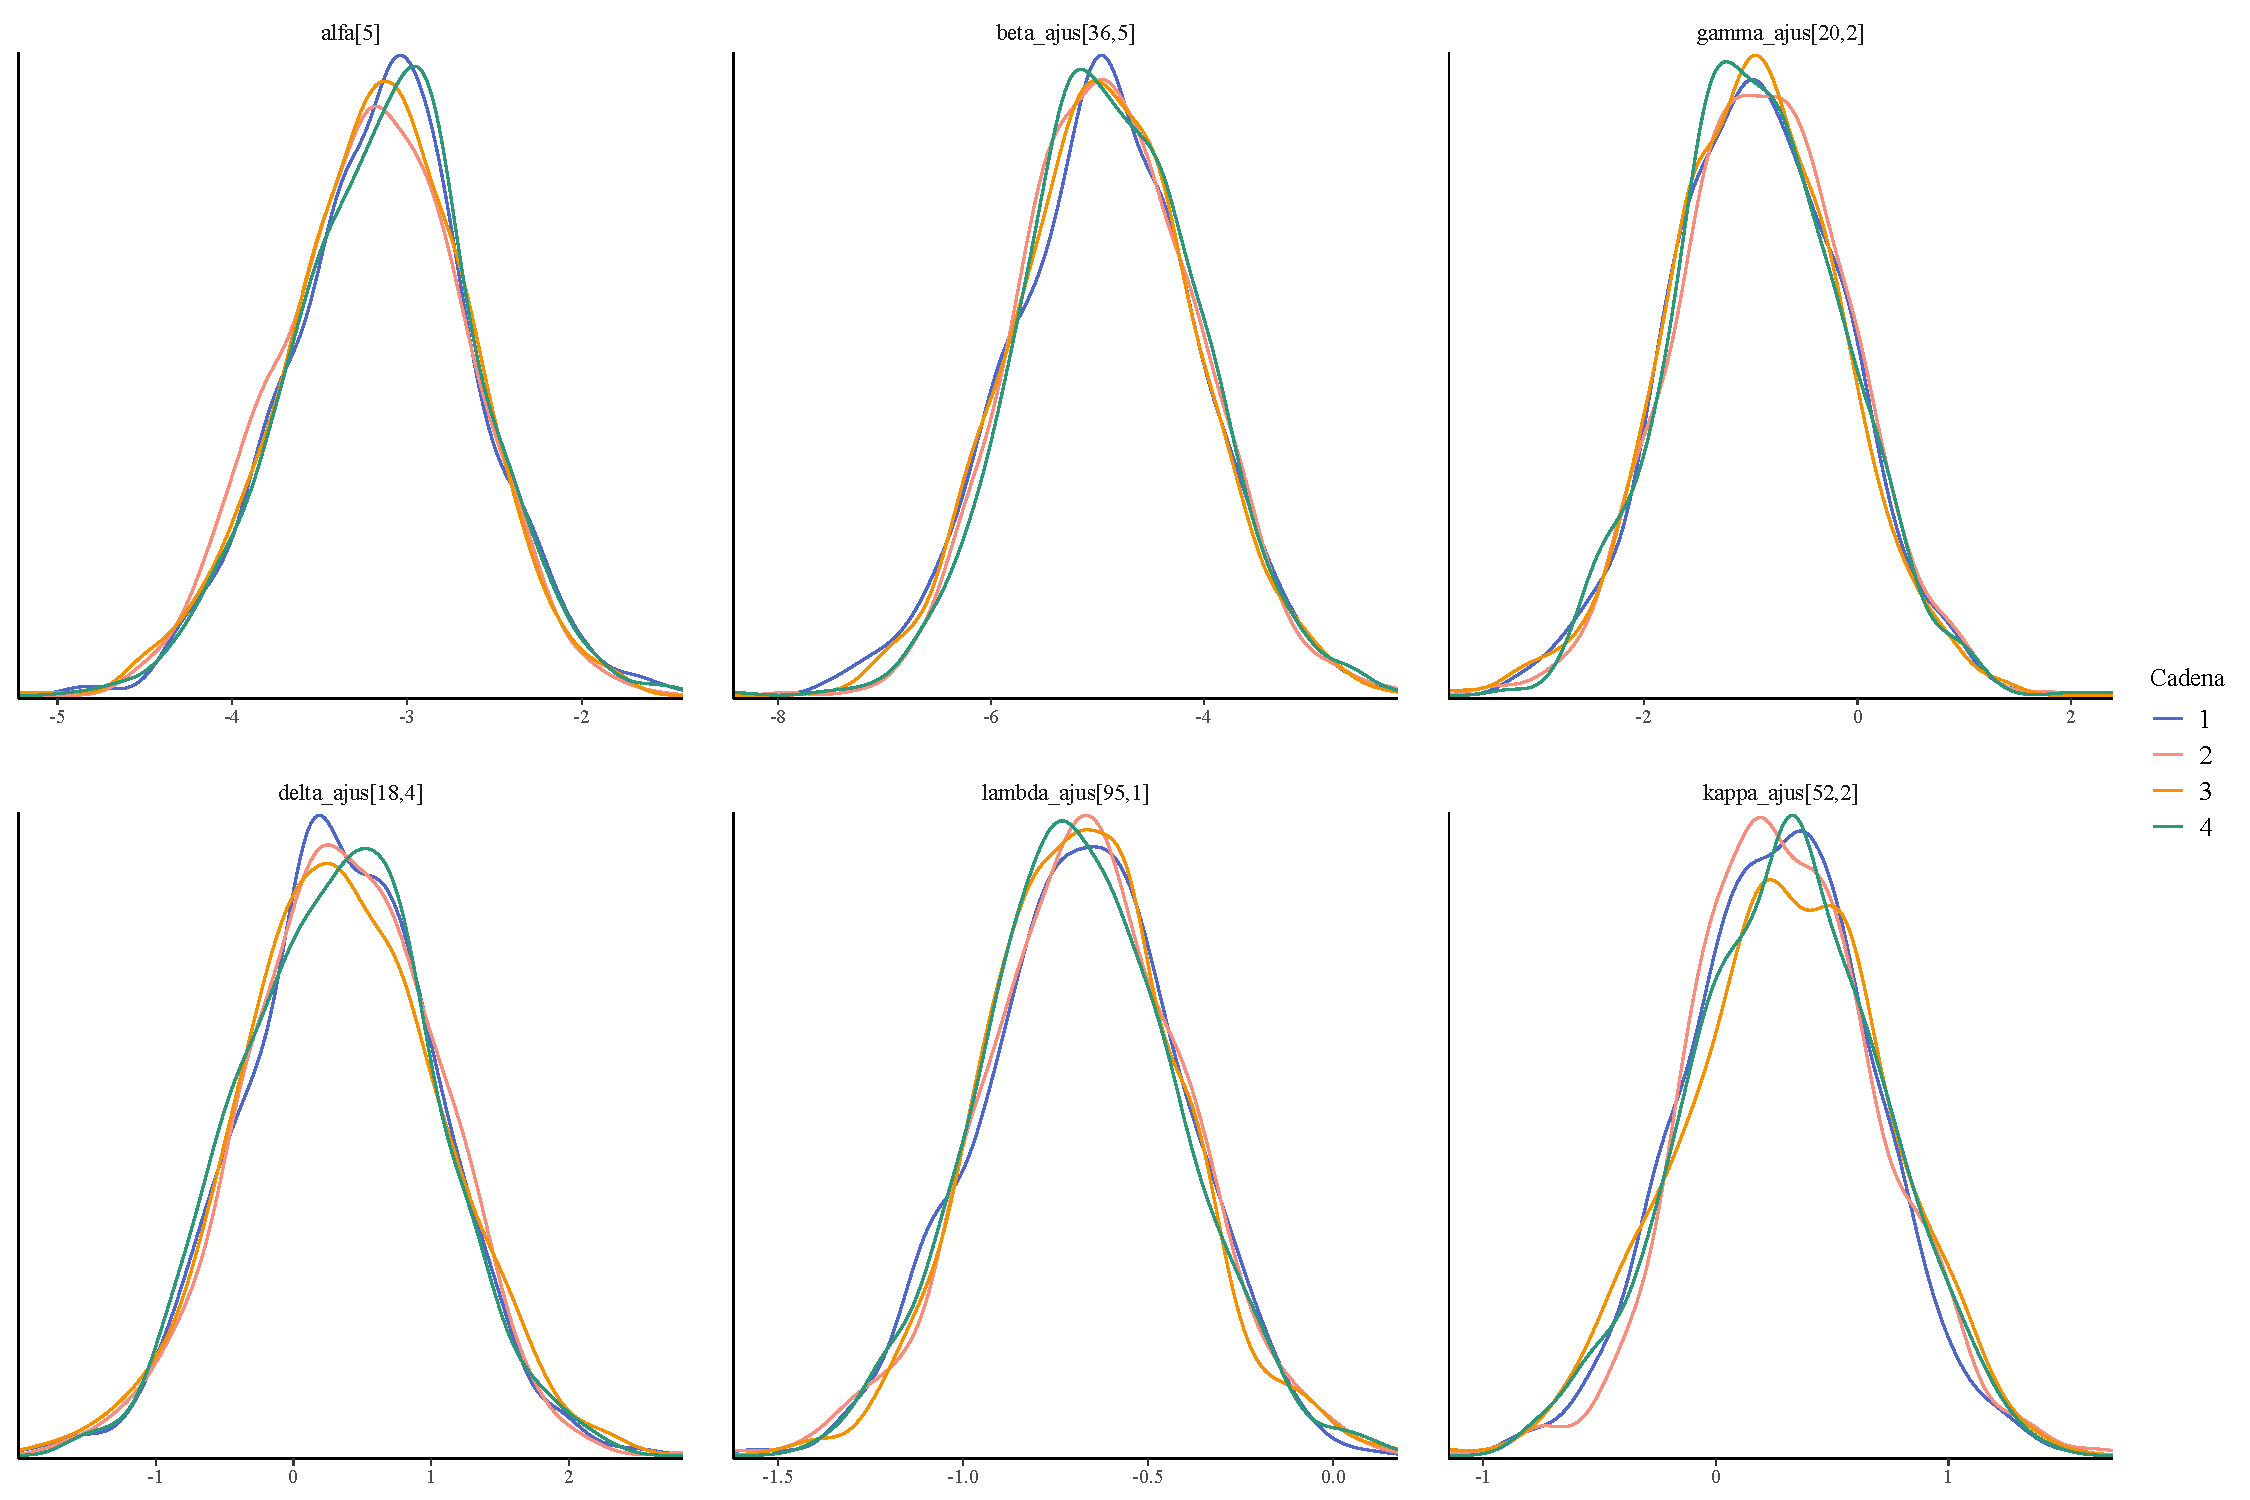
\includegraphics[width = \textwidth]{Figs/Convergencia/Convergencia_Densidades}
	\caption{Ejemplo de gráficos de densidades por cadena para algunos parámetros del modelo H.}
	\label{fig:Densidades_H}
	\end{subfigure}
	~
	\begin{subfigure}{0.6\textwidth}
	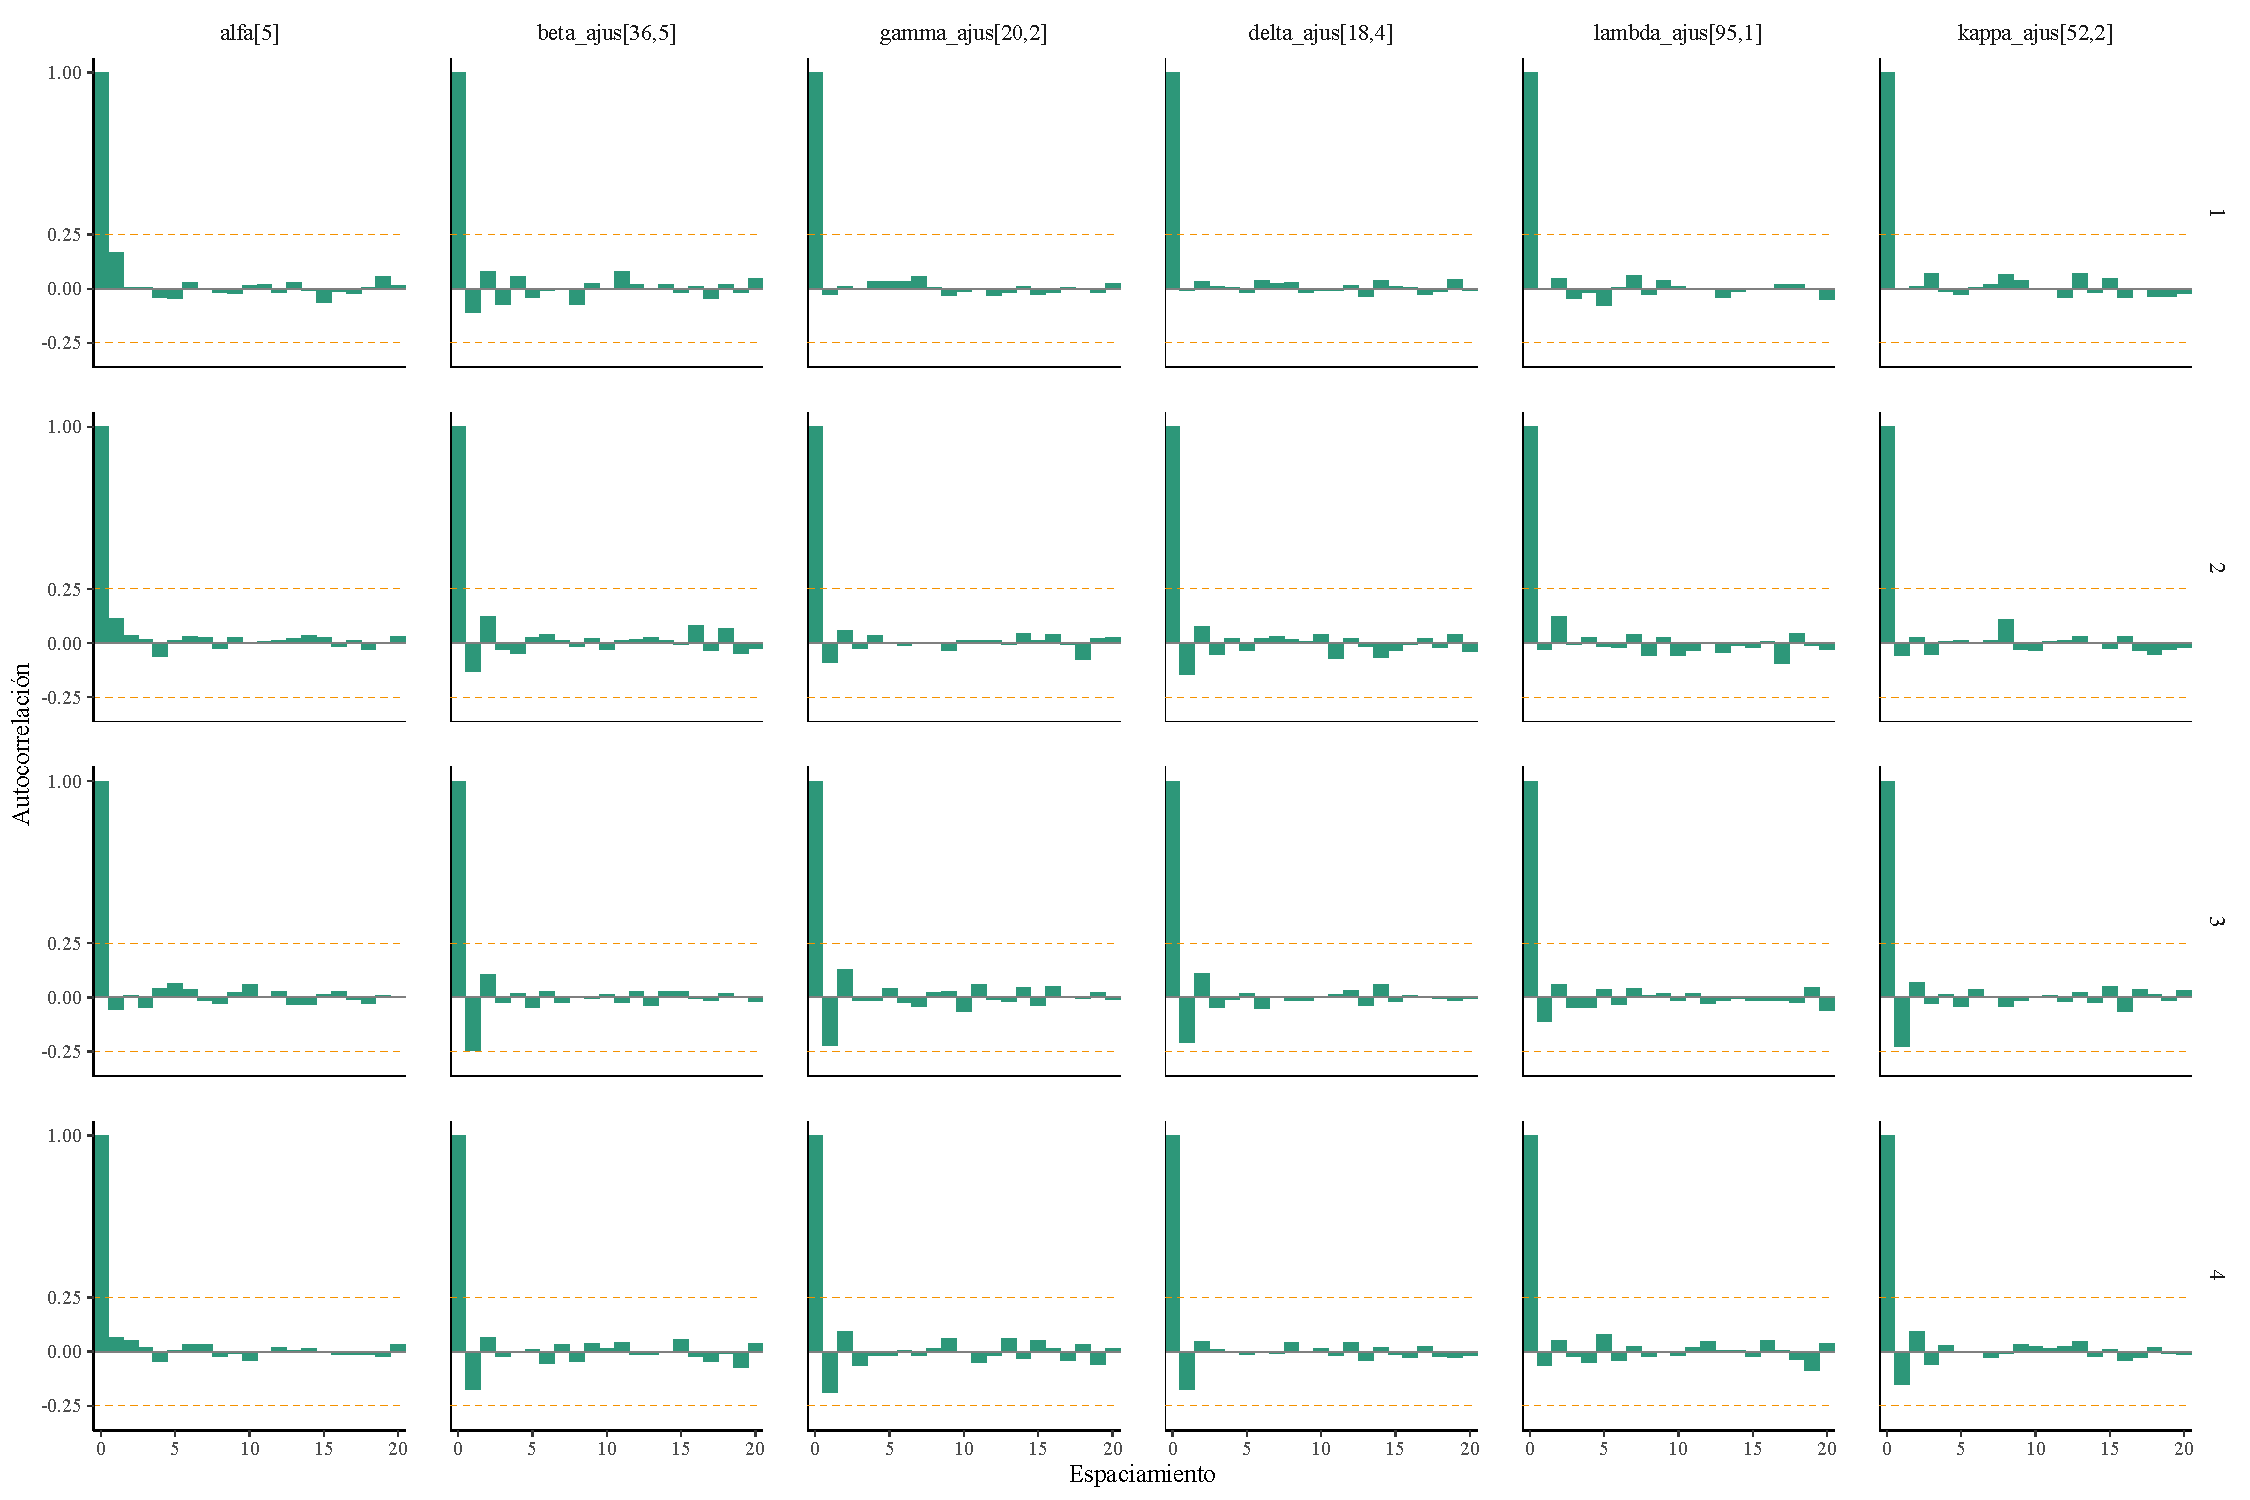
\includegraphics[width = \textwidth]{Figs/Convergencia/Convergencia_AutoCorr}
	\caption{Ejemplo de gráficos de autocorrelación para algunos parámetros del modelo H.}
	\label{fig:Autocorr_H}
	\end{subfigure}
	\caption{Fuente: elaboración propia.}
\end{figure}

 También analicé la convergencia del modelo H mediante los diagnósticos del paquete de $\mathsf{R}$ \textit{shinystan}, que permite de manera interactiva observar distintos gráficos y resúmenes respecto al ajuste del modelo vía HMC. De esta exploración, también concluí que el modelo satisfacía suficientemente bien la batería de diagnósticos para darnos confianza en que las muestras obtenidas provienen de la distribución posterior.\\
 
 En este punto conviene discutir un pequeño análisis de sensibilidad que realicé tomando en cuenta que los modelos considerados incorporan distribuciones iniciales informativas. ¿Qué pasa si utilizamos una inicial vaga como la $N(0,100)$ que discutí en la \textbf{\autoref{Secc_Iniciales}}? Realicé una nueva corrida del modelo H con todas las distribuciones iniciales $N(0,100)$, pero utilizando la misma semilla, el mismo número de cadenas, iteraciones y parámetros para la implementación de HMC de Stan. Llamo a esta nueva corrida el \textbf{Modelo S}, por sensibilidad.\\
  
 Lo primero que debe decirse es que las iniciales no informativas dañan significativamente la eficiencia del muestreo por HMC. Consideremos que el Modelo H tardó aproximadamente 9 horas con 11 minutos en terminar las 4000 simulaciones posteriores divididas en 4 cadenas de 1000 iteraciones de calentamiento y 1000 de muestreo cada una. ¡El Modelo S tardó 34 horas! Más aún, aunque los principales diagnósticos de convergencia indican que también el modelo S convergió, a diferencia de los modelos con iniciales informativas, este modelo sí generó advertencias en algunos diagnósticos.\\
 
 En primer lugar, cada iteración de HMC del modelo S siempre llegó a lo que podríamos considerar como el tiempo máximo de integración de las trayectorias hamiltonianas y que en Stan se conoce como \textit{max treedepth}. La forma de resolver esta advertencia es aumentando el máximo permitido pero esto lleva consigo un mayor tiempo de cómputo, mismo que ya podría considerarse excesivo comparado con el modelo H. Por otro lado, vemos que las autocorrelaciones en el modelo S son mucho mayores que en el modelo H--- comparar \textbf{Figuras  \ref{fig:Autocorr_H}, \ref{fig:Autocorr_S}}---. Como consecuencia, los tamaños efectivos de muestra son siempre menores en el modelo S que en el modelo H, como puede observarse en la \textbf{Figura \ref{fig:N_eff_compara}}. Esto querría decir que los estimadores del modelo S tienen un mayor error de Monte Carlo que los del modelo H. De hecho, Stan automáticamente imprime una advertencia para el modelo S haciendo notar que las medias y medianas posteriores pudieran no ser confiables debido al tamaño de muestra.\\
 
 \begin{figure}[h]
	\centering
	\begin{subfigure}{0.45\textwidth}
	\includegraphics[width = \textwidth]{Figs/Convergencia/Convergencia_Traceplots_s}
	\caption{Ejemplo de \textit{traceplots} para los mismos parámetros del modelo S que se seleccionaron para el modelo H.}
	\label{fig:Traceplots_S}
	\end{subfigure}
	~
	\begin{subfigure}{0.45\textwidth}
	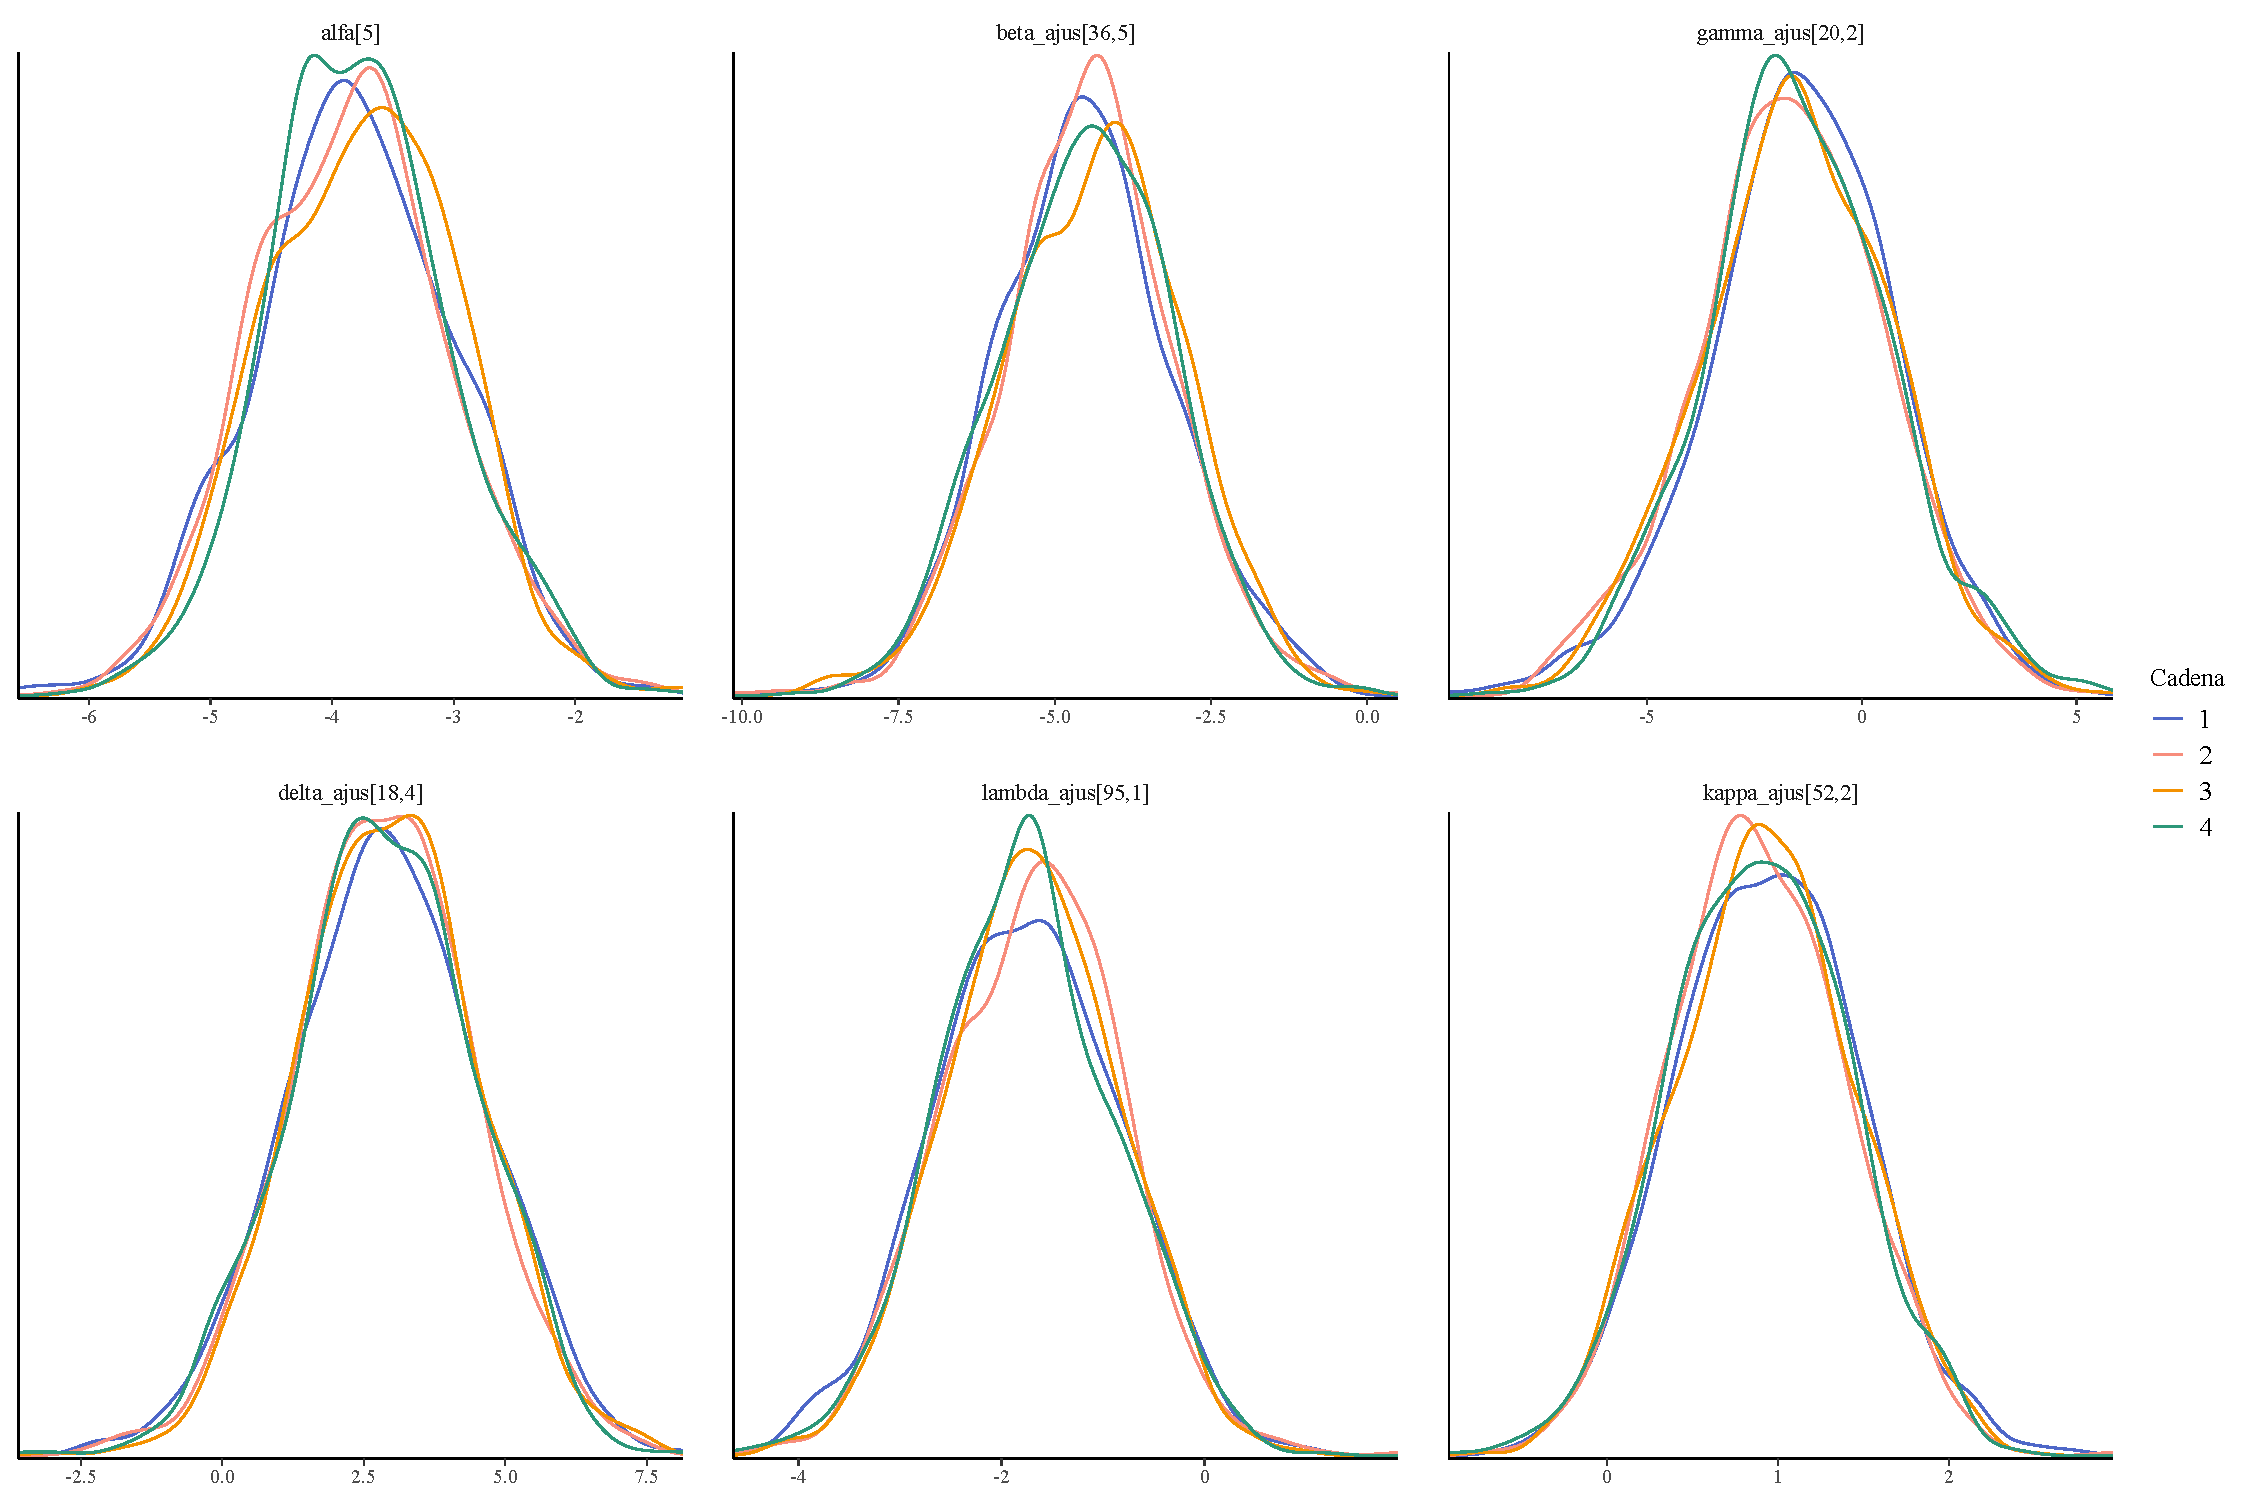
\includegraphics[width = \textwidth]{Figs/Convergencia/Convergencia_Densidades_S}
	\caption{Ejemplo de gráficos de densidades para los mismos parámetros del modelo S que se seleccionaron para el modelo H.}
	\label{fig:Densidades_S}
	\end{subfigure}
	~
	\begin{subfigure}{0.6\textwidth}
	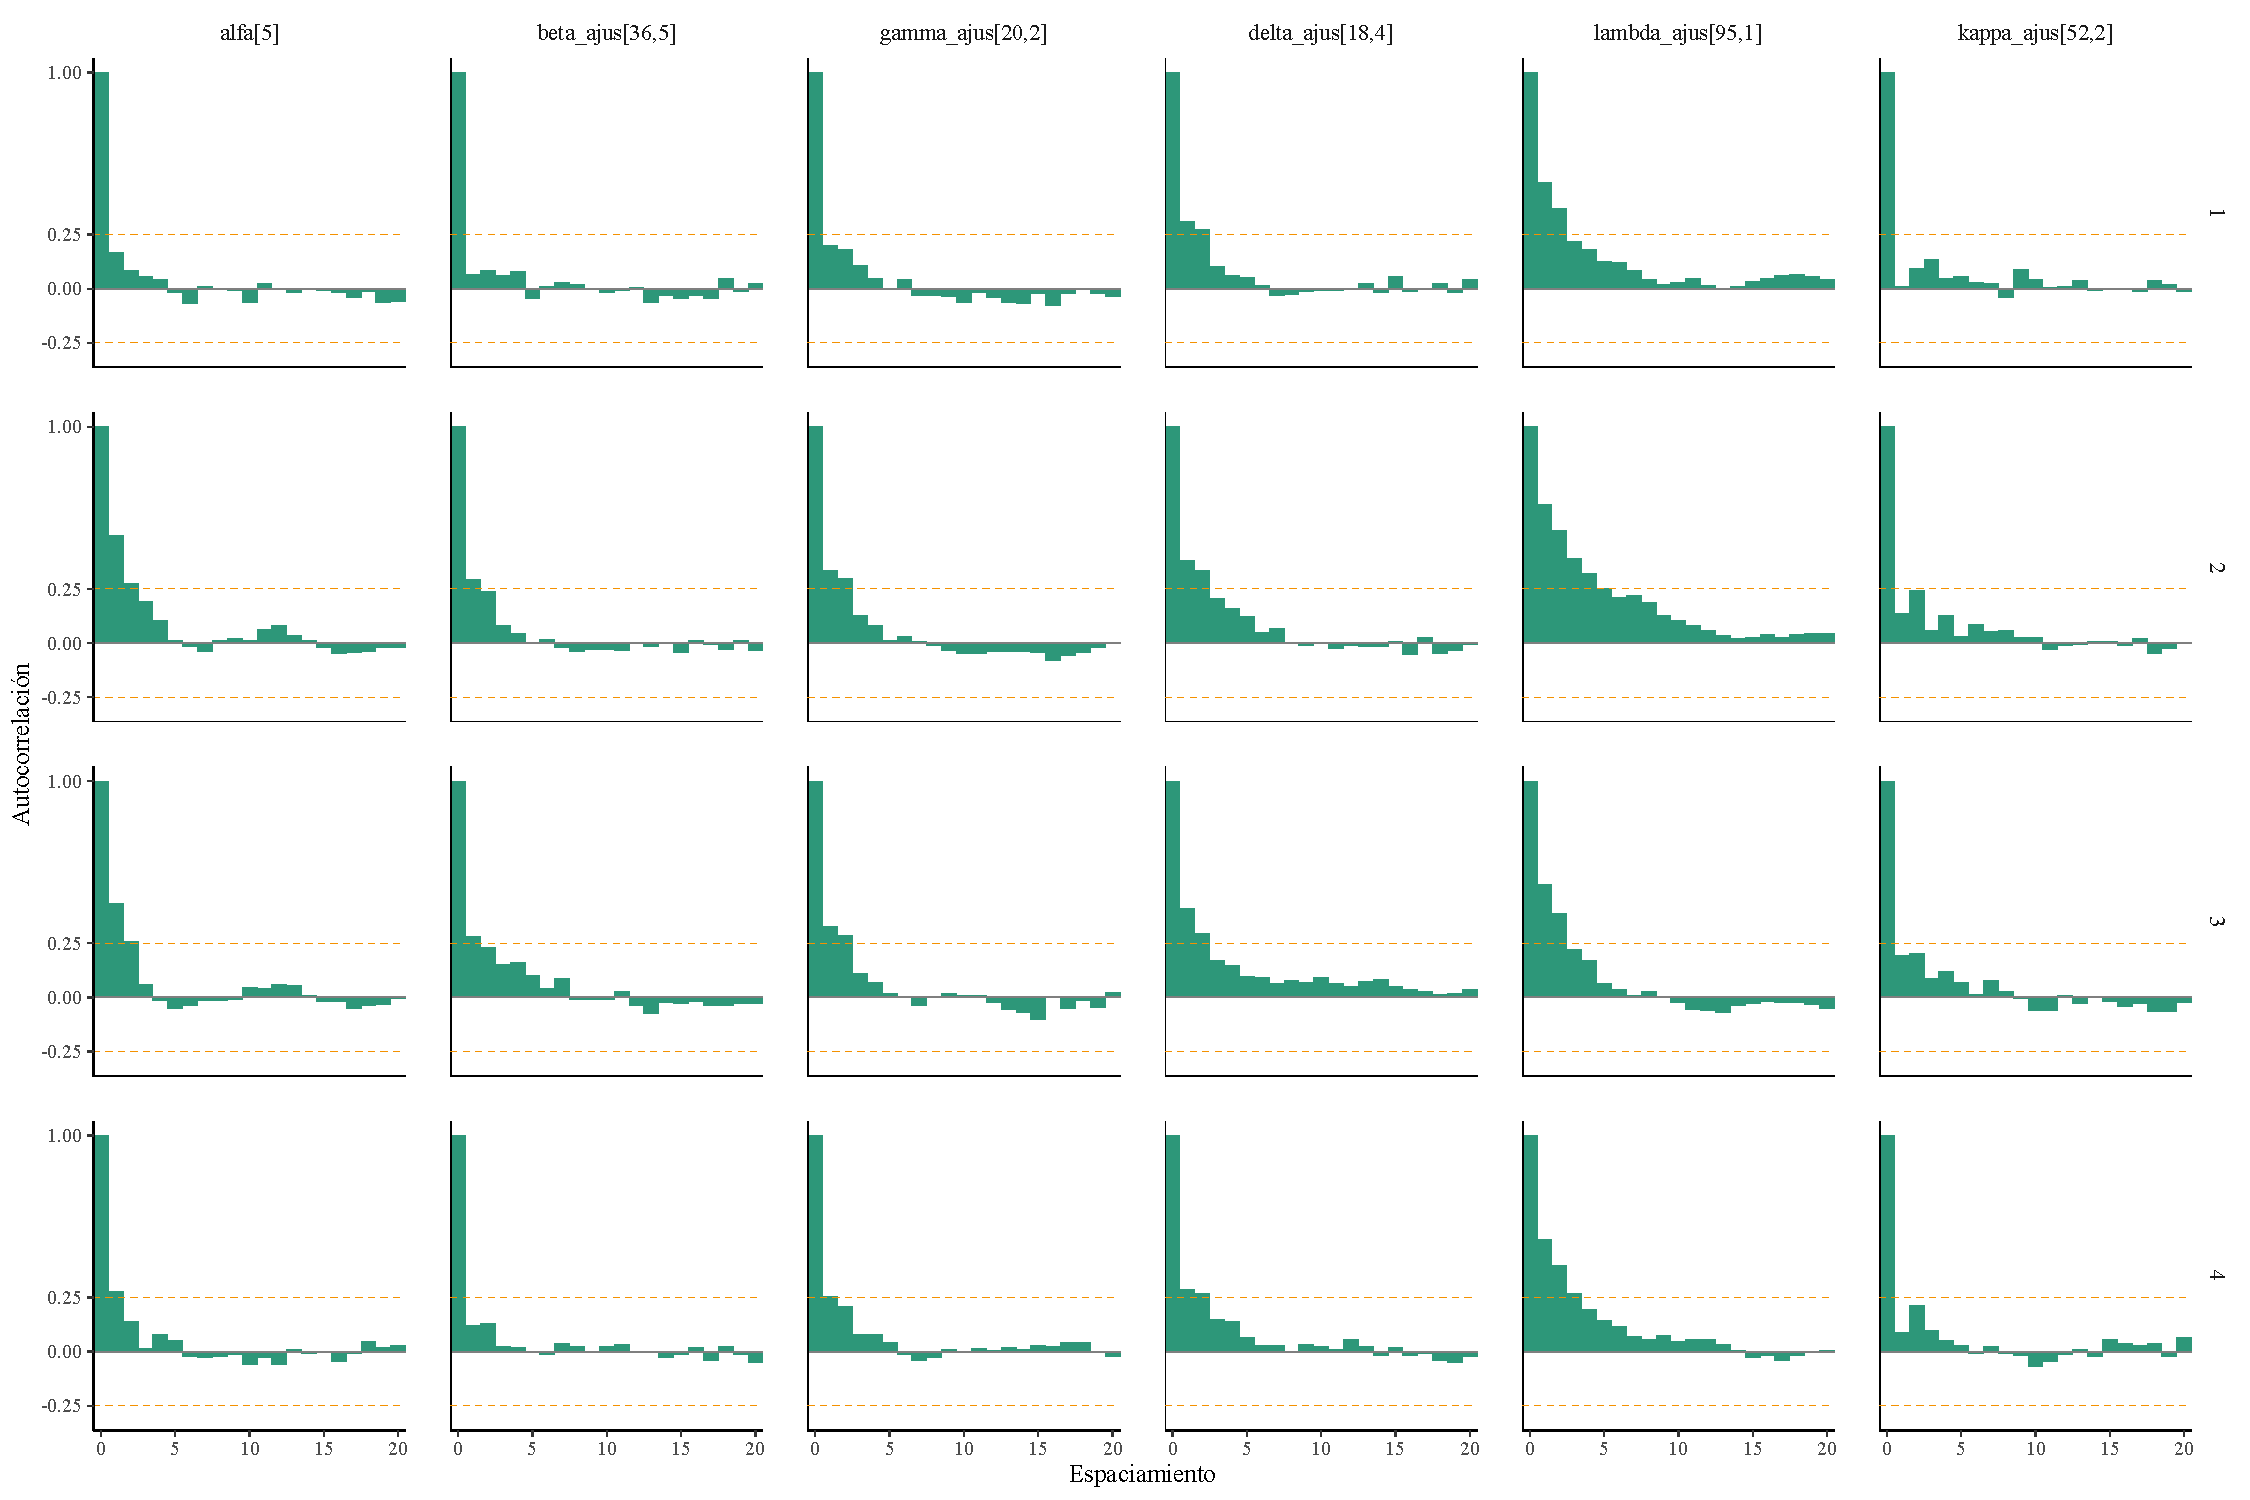
\includegraphics[width = \textwidth]{Figs/Convergencia/Convergencia_AutoCorr_S}
	\caption{Ejemplo de gráficos de autocorrelación para los mismos parámetros del modelo S que se seleccionaron para el modelo H.}
	\label{fig:Autocorr_S}
	\end{subfigure}
	\caption{Fuente: elaboración propia.}
\end{figure} 
 
 Adicionalmente, observamos en la \textbf{Figura \ref{fig:Rhat_compara}} que los factores de reducción de escala tienden a ser mayores para el modelo S que para el modelo H. Si bien todos son lo suficientemente cercanos a 1 como para declarar convergencia con base en este diagnóstico, sí podemos reafirmar que tendríamos más confianza en los valores del modelo H que en los del S. Esto también podría decirse comparando las densidades para los parámetros seleccionados en las \textbf{Figuras  \ref{fig:Densidades_H}, \ref{fig:Densidades_S}}. Las estimaciones de las cadenas del modelo H son más parecidas entre sí que aquellas del modelo S. Finalmente, comparando los traceplots de los modelos (\textbf{Figuras  \ref{fig:Traceplots_H}, \ref{fig:Traceplots_S}}) observamos cómo en la fase de calentamiento el modelo S pasa más tiempo explorando regiones poco creíbles del espacio parametral--- recordemos que no esperaríamos efectos superiores en magnitud a 5 en la escala logística--- pero que las iniciales vagas sugieren. Ciertamente las cadenas terminan por ``encontrar'' la región crítica, pero este puede no ser siempre el caso cuando se consideran las restricciones de tiempo que se tengan en alguna aplicación dada o cuando se usan iniciales aún más vagas.\footnote{No se presenta por brevedad pero con los mismos parámetros un modelo con iniciales $N(0,10000)$ no logra converger en las 2000 iteraciones y sus 4 cadenas no mezclan pues siguen explorando regiones alejadas del espacio parametral.}\\ 
 
 
\begin{figure}[H]
	\centering
	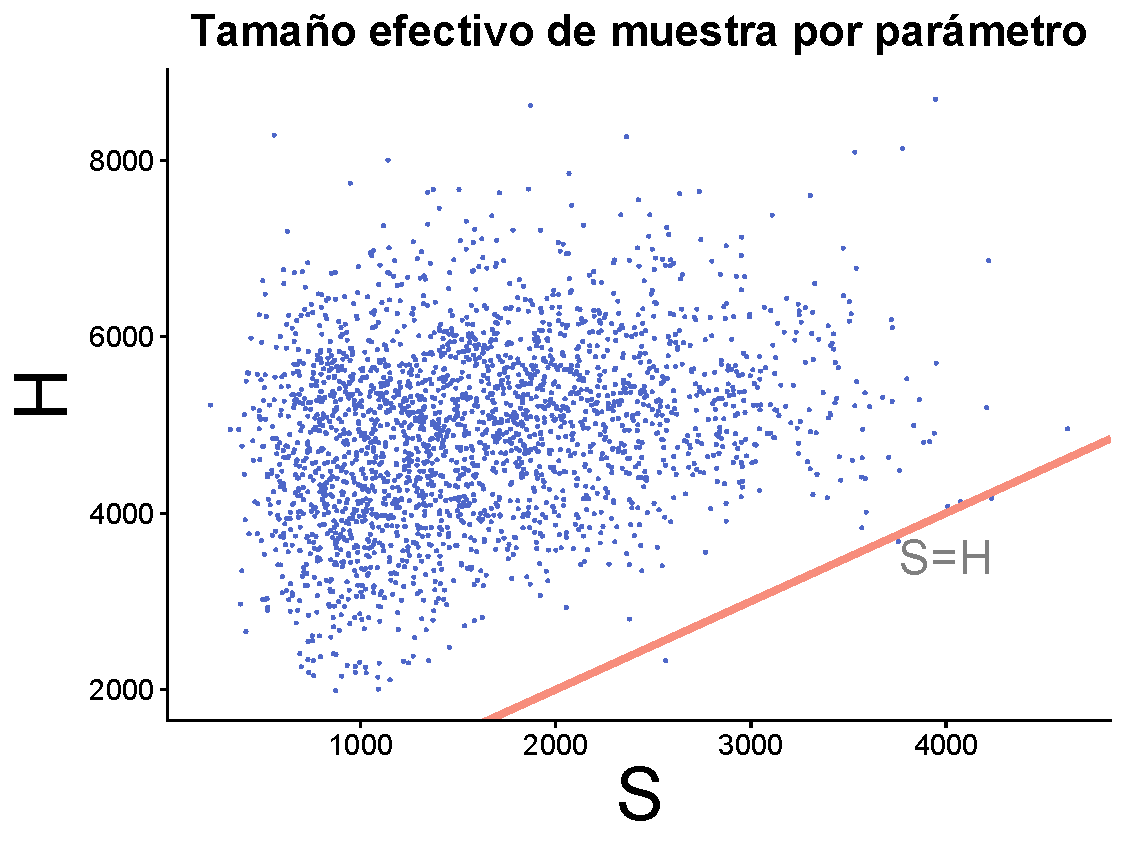
\includegraphics[width = 0.9\textwidth]{Figs/Convergencia/Compara_n_eff}
	\caption{Comparativo de tamaños efectivos de muestra para los modelos H y S. Fuente: elaboración propia.}
	\label{fig:N_eff_compara}
\end{figure} 

\begin{figure}[H]
	\centering
	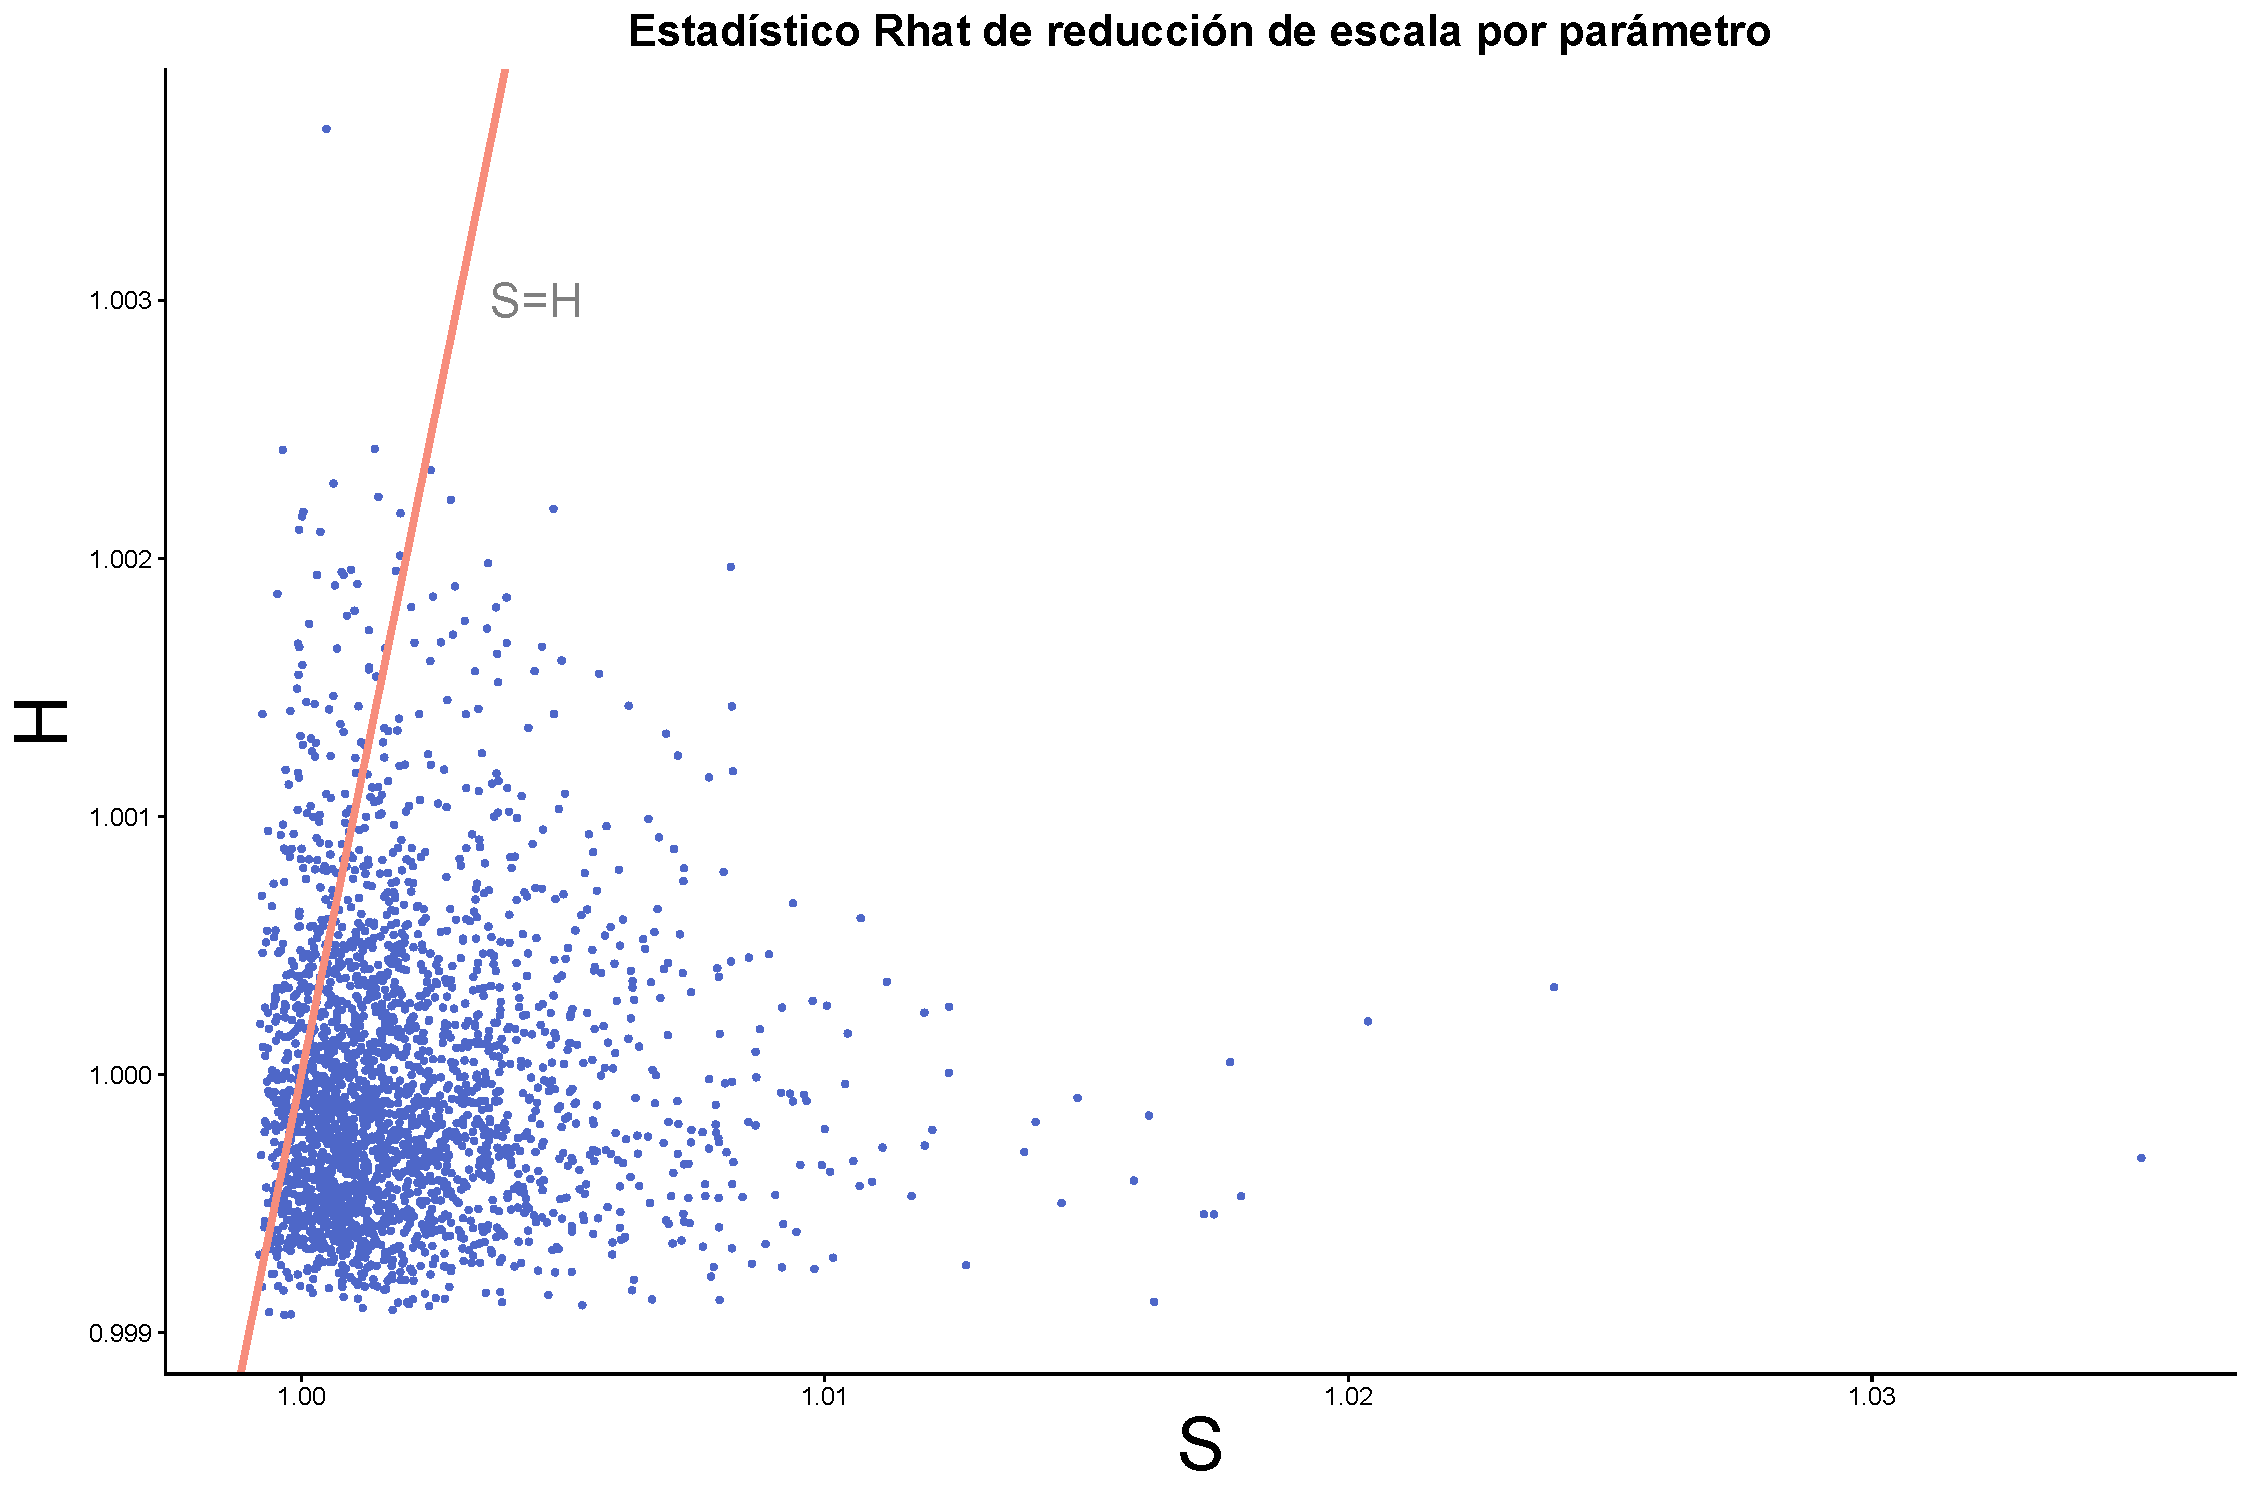
\includegraphics[width = 0.9\textwidth]{Figs/Convergencia/Compara_Rhat}
	\caption{Comparativo de factores de reducción de escala para los modelos H y S. Fuente: elaboración propia.}
	\label{fig:Rhat_compara}
\end{figure} 
 
  Por todo lo anterior, seleccionamos al modelo H como el modelo final a analizar. Por lo que, una vez verificada su convergencia, podemos proceder con confianza al análisis de los resultados. Para ello debemos interpretar lo que los coeficientes estimados nos dicen. 
 
\section{Efectos de las variables}

Interpretar los coeficientes de regresiones logísticas no es sencillo pues, por la función liga, estos se encuentran en una escala distinta a la de las proporciones o probabilidades que es en la que normalmente estamos interesados. Como explican \textcite{GelmanHill06}, además de las interpretaciones en términos de momios, una primera alternativa es considerar el caso cuando la variable explicativa vale 1. Sin embargo, esto no siempre tiene sentido dependiendo del contexto en el que se realiza la regresión. Sobre todo para evitar alguna falacia ecológica--- ver página \pageref{No_Extrapolar}--- yo no podría interpretar los coeficientes mediante alguna estrategia de ese tipo.\\ 

 Por ello, resultan útiles lo que los mismos autores llaman \textit{predictive comparisons}. Básicamente estos consisten en pensar en los efectos de los coeficientes en términos de una comparación entre dos valores distintos pero informativos de las variables explicativas de interés; por ejemplo, la media y una desviación estándar por encima de ella. Esta elección tiene la ventaja de que, usualmente, se estaría realizando la interpretación en el rango de valores observado y no mediante una extrapolación. Hay que decir, no obstante, que una situación donde esto puede no suceder es cuando las variables observadas sean multimodales y la media caiga en uno de los valles. Esta discusión general sobre alternativas de interpretación para regresiones logísticas puede consultarse en la referencia antes citada.\\ 
 
\subsection{Definiendo efectos}

 Por nuestra parte, para fijar ideas, recordemos que las variables explicativas son las \textit{configuraciones sociales} definidas por las categorías poblacionales de las variables censales. Supongamos por ahora que quisiéramos analizar un modelo individual nacional para una variable con 3 categorías, $x = (x_1,x_2,x_3)$.\footnote{La interpretación se realizará solo para le modelo compuesto H, pero para entender la interpretación de efectos conviene empezar planteándola para un modelo más sencillo.} Recordando \eqref{eq:Modelo_Nal_Ind} y omitiendo por claridad algunos subíndices, tendríamos que para alguna comuna en particular,

\begin{equation*}
ln\left(\dfrac{p}{1-p}\right) = \alpha + \beta_1 x_1 + \beta_2 x_2 + \beta_3 x_3.
\end{equation*}

Abusando de la notación, introduzco ahora unas expresiones. En primer lugar

\begin{equation*}
\eta(x;\beta_i)= \alpha + \beta_i x_i + \sum\limits_{k\neq i} \beta_k x_k, 
\end{equation*} 

para referirme al predictor lineal como función de la configuración social $x$ y considerando el intercepto $\alpha$ y los coeficientes como fijos; pongo énfasis en el coeficiente $\beta_i$ porque es el efecto a interpretar. Asimismo tomemos 

\begin{equation*}
p(x;\beta_i)=\dfrac{e^{\eta(x;\beta_i)}}{1+e^{\eta(x;\beta_i)}}=\dfrac{1}{1+e^{-\eta(x;\beta_i)}}
\end{equation*} 

como el valor de la afinidad por Marine Le Pen en la comuna como función de la configuración social y, de nuevo, con el resto del predictor lineal fijo.\\

 Buscaríamos entonces definir el efecto que tiene el coeficiente $\beta_i$ como el cambio en puntos porcentuales para dicha afinidad cuando se pasa de una configuración a otra. Por ejemplo, suponiendo $x_{(0)}$ como una configuración inicial y $x_{(1)}$ como otra en la que aumenta la categoría de interés, tendríamos que el efecto sería

\begin{equation*}
\Delta(\beta_i;x_{(0)},x_{(1)}) = p(x_{(1)};\beta_i)-p(x_{(0)};\beta_i)
\end{equation*}

Sin embargo, en nuestro caso no tenemos total libertad para elegir los valores $x_{(0)}$ y $x_{(1)}$ pues recordemos que son proporciones que deben sumar a 1. ¿Cómo elegirlos entonces?\\ 

En primer lugar, podemos seleccionar el punto de referencia $x_{(0)}$ como la media muestral, $x_{(0)}=\bar{x}=(\bar{x}_1,\bar{x}_2,\bar{x}_3)$. Posteriormente, como estamos interesados en el efecto del coeficiente $\beta_i$, empecemos a construir $x_{(1)}$ con base en $x_{(1),i}=\bar{x}_i + s_i$ donde $s_i$ es la desviación estándar muestral en la $i$-ésima categoría. Al agregarle una desviación estándar a $x_i$, para cumplir con la restricción, debemos disminuir su valor del resto de las $x_k$ en su conjunto. Sin que sea la única forma de hacerlo, una propuesta es quitarle de manera proporcional a cada categoría restante una parte de la desviación estándar que sumamos a la categoría de interés. Esto sería de la siguiente manera: 

\begin{equation*}
x_{(1),k}=\bar{x}_k - s_i \dfrac{\bar{x}_k}{1-\bar{x}_i} \quad \forall k \neq i
\end{equation*}

Con este criterio podemos abusar un poco más de la notación. Si en lugar del caso específico de una configuración social de 3 categorías tenemos $l$, el efecto sería 

\begin{align*}
\Delta(\beta_i) &= p(x^\star;\beta_i)-p(\bar{x};\beta_i) \quad \forall i \in \mathbb{N}_l \\
\text{donde} \quad \bar{x} &= (\bar{x}_1,\dots,\bar{x}_{l}), \\ 
x_i^\star = \bar{x}_i + s_i \quad &\text{y} \quad x_j^\star =\bar{x}_j - s_i\dfrac{\bar{x}_j}{1- \bar{x}_i} \quad \forall j \neq i 
\end{align*}

La interpretación de los coeficientes sería entonces el efecto predicho en puntos porcentuales al aumentar la proporción de individuos en la categoría de interés respecto a una comuna ``típica''; es decir, al pasar de $\bar{x}$ a $x^\star$.\\ 

Ahora pensemos que querríamos calcular efectos para nuestros modelos jerárquicos. En este caso en lugar de un solo efecto nacional $\Delta(\beta_i)$ tendríamos 96 efectos $\Delta(\beta_{d,i})$, uno para cada departamento. Por lo mismo, simplemente reemplazamos el parámetro de interés por su equivalente jerárquico y tendríamos que calcular la media, $\bar{x}_{d}$, y la desviación estándar correspondiente dentro de cada departamento, $s_{d,i}$: 

\begin{equation*}
\Delta(\beta_{d,i}) =  p(x^\star_{d};\beta_{d,i})-p(\bar{x}_{d};\beta_{d,i}) \quad \forall i \in \mathbb{N}_l
\end{equation*}

¿Pero qué pasa cuando tenemos un modelo compuesto con más de una variable censal? En esta situación, la decisión que tomé fue buscar una comparación \textit{c\ae teris paribus} en la que los sumandos del resto de variables explicativas del predictor lineal toman sus valores promedio en el departamento. Podemos también pensar que estamos modificando el intercepto con los sumandos del resto de categorías con valores promedio. Por ello, si asociamos a $x$ con la variable de la categoría de interés, $\theta$ con sus coeficientes y $z$ con el resto del predictor lineal, una notación más general podría ser

\begin{align}\label{eq:Efecto_Enchufado_Compuesto}
\Delta(\theta_{d,i};\bar{z}_d) &= p(x_d^\star;\theta_{d,i},\bar{z}_d)-p(\bar{x}_d;\theta_{d,i},\bar{z}_d) \quad \forall i \in \mathbb{N}_l \\
\text{donde} \quad p(x_d;\theta_{d,i},\bar{z}_d) &=\dfrac{1}{1+e^{-\eta(x_d;\theta_{d,i},\bar{z}_d)}} \nonumber \\
\text{y} \quad \eta(x_d;\theta_{d,i},\bar{z}_d) &= \bar{z}_d + \theta_{d,i}x_{d,i} + \sum\limits_{k\neq i} \theta_{d,k}x_{d,k}. \nonumber
\end{align}

Por ejemplo, pensemos en el caso del modelo compuesto A que incluye a la escolaridad y a las categorías socioprofesionales. Si queremos el efecto para una categoría de escolaridad, $\theta = \beta$ y este dependería del intercepto y las 8 categorías socioprofesionales vía $\bar{z}_d = \alpha_d + \sum\limits_{j=1}^8 \gamma_{d,k}\bar{x}_{csp,d,k}$. Análogamente, para el efecto de una categoría socioprofesional tendríamos $\theta = \gamma$ y $\bar{z}_d = \alpha_d + \sum\limits_{j=1}^5 \beta_{d,k}\bar{x}_{escol,d,k}$.\\

Hasta aquí ya construimos una propuesta de efecto comparando dos predicciones específicas del modelo ``enchufando'' un valor específico o un estimador puntual de los coeficientes. Sin embargo, tenemos incertidumbre sobre sus valores reflejada mediante muestras posteriores de $S$ valores simulados via HMC. Por lo mismo, siguiendo la única receta de la estadística bayesiana tendríamos que obtener la distribución posterior de los efectos, calculando \eqref{eq:Efecto_Enchufado_Compuesto} para cada simulación posterior $\beta_{d,i}^{(s)}$ y, correspondientemente, $\bar{z}_d^{(s)}$:

\begin{equation*}
\Delta(\beta_{d,i}^{(s)};\bar{z}_d^{(s)}) =  p(x^\star_{d};\beta_{d,i}^{(s)},\bar{z}_d^{(s)})-p(\bar{x}_{d};\beta_{d,i}^{(s)},\bar{z}_d^{(s)}) \quad \forall i \in \mathbb{N}_l ,\, s \in \mathbb{N}_S.
\end{equation*}

Esta sería la distribución posterior de los efectos con la que podemos continuar el análisis de los modelos mediante distintos resúmenes inferenciales como el efecto mediano. Asimismo, podemos resumir la distribución reportando intervalos centrales de probabilidad al 95\% y, siguiendo la práctica común, cuando estos contengan al 0, diremos que la categoría poblacional no tiene un efecto significativo. Si, por el contrario, se encuentran en su totalidad por encima o por debajo del 0, diremos que se tiene un efecto significativo positivo o negativo, respectivamente.

\subsection{Escolaridad}

Comienzo el análisis de los efectos predichos por el modelo final por la variable de escolaridad, pues era la que los modelos individuales sugerían como más explicativa y sobre la que se fue construyendo el modelo 0 hasta llegar al H. En la \textbf{Figura \ref{fig:Mapa_Efectos_Escolaridad}} podemos observar el mapa de estimadores puntuales para los efectos departamentales por categorías de escolaridad bajo el modelo H. En cada departamento la intensidad de color refleja la magnitud del efecto mediano; en tonos rojos tenemos efectos negativos y en tonos azules efectos positivos.\\

\begin{figure}[h]
	\centering
	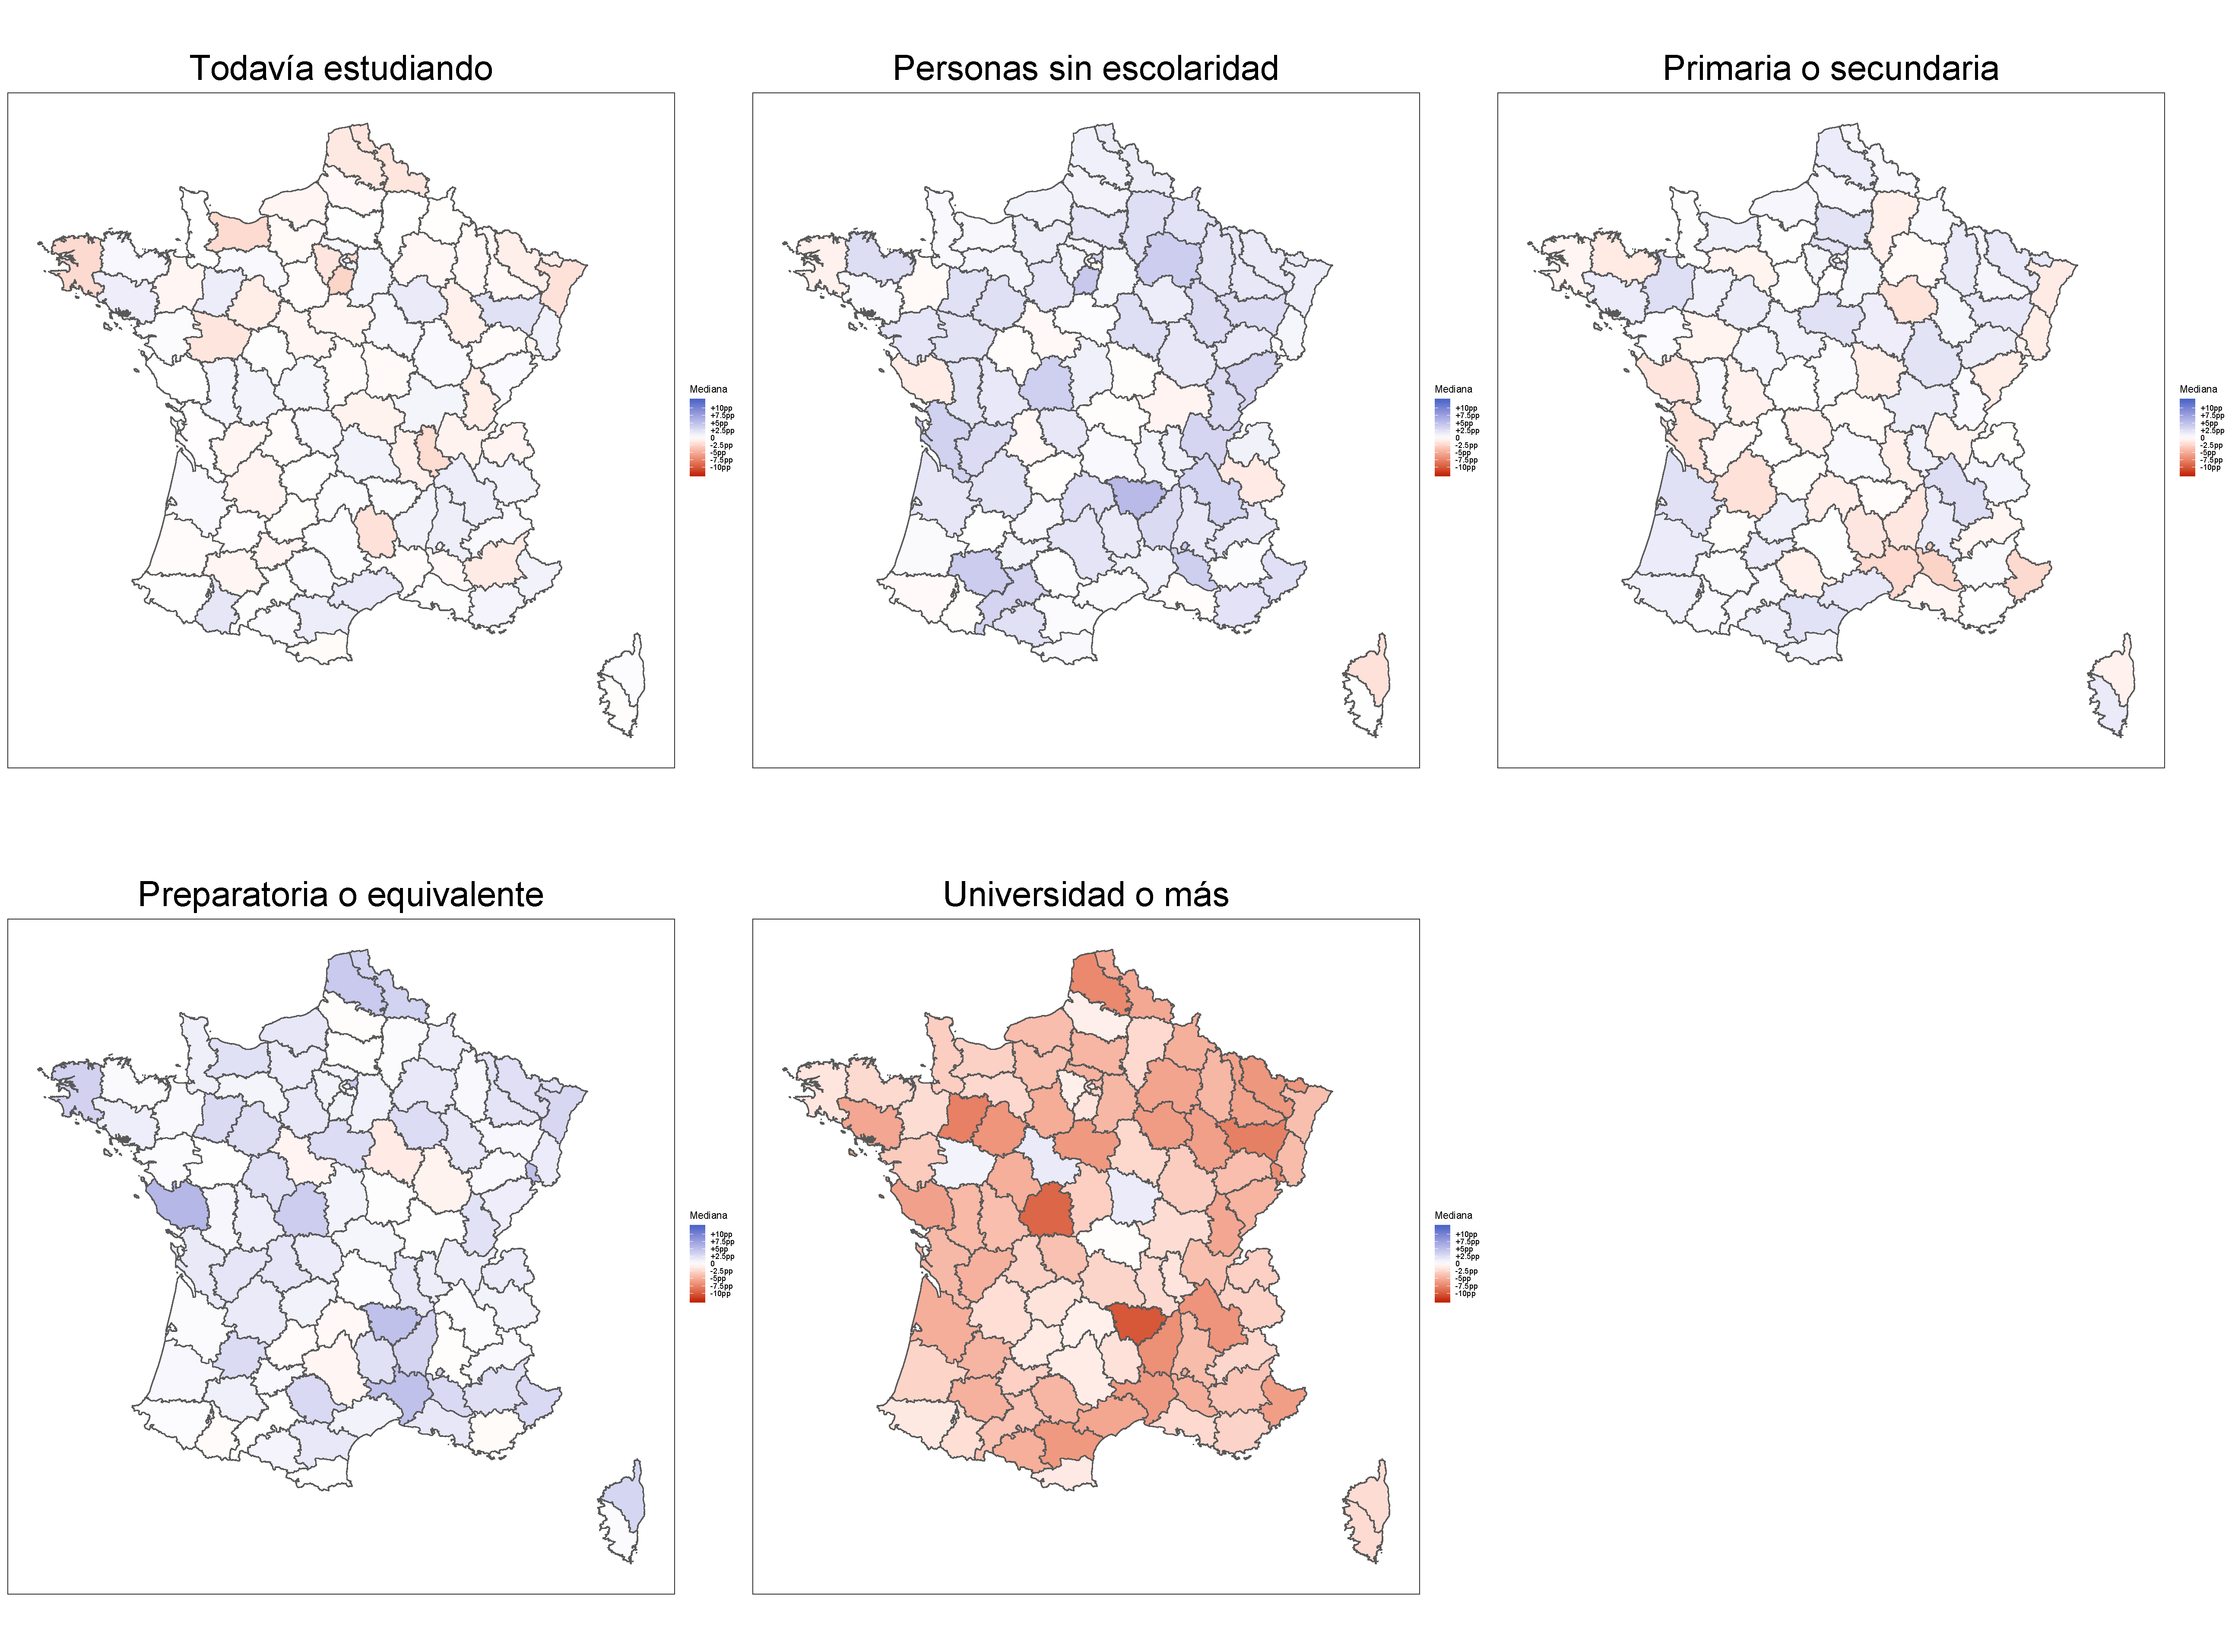
\includegraphics[width = 0.9\textwidth]{Figs/Efectos/Mapa_Efectos_Escolaridad_Modelo_H}
	\caption{Estimaciones puntuales de los efectos de la escolaridad por departamento francés bajo el modelo H. Fuente: elaboración propia con la cartografía de Open Street Map.}
	\label{fig:Mapa_Efectos_Escolaridad}
\end{figure}

Inmediatamente observamos que la categoría universidad o más tiene un efecto negativo en prácticamente todo el hexágono francés. Algunos departamentos tienen magnitudes altas, reflejadas en la intensidad del color. Por el contrario, el aumento en el porcentaje de personas sin escolaridad parece llevar consigo un aumento en las preferencias por Marine Le Pen en la mayoría de departamentos. No obstante, vemos que en Córcega se daría el efecto contrario. En tonos más claros, es decir con una magnitud menor, el porcentaje de personas con escolaridad equivalente a la preparatoria parece también tener un efecto positivo en la afinidad por el FN. Los mapas de las personas que todavía están estudiando y de personas con primaria o secundaria parecen tener efectos mixtos, aunque los segundos se observan más intensos que los primeros.\\

Ahora bien, estos son solo estimadores puntuales. Una de las principales ventajas de los modelos jerárquicos bayesianos es que nos permiten reconocer la variabilidad de los fenómenos bajo estudio así como reportar la incertidumbre sobre ellos de manera más clara. En la \textbf{Figura \ref{fig:Efectos_Escolaridad}} tenemos un resúmen de las distribuciones posteriores de los efectos. Para cada categoría observamos las 96 distribuciones posteriores representadas mediante intervalos centrales de probabilidad al 95\%, 80\% y 50\% así como la mediana como estimador puntual que ordena los departamentos por categoría. Si el efecto se estima significativo--- es decir que el intervalo al 95\% excluye al 0---, observamos la distribución marcada en rosa o azul dependiendo del sentido de dicho efecto.\\
  
\begin{figure}[h]
	\centering
	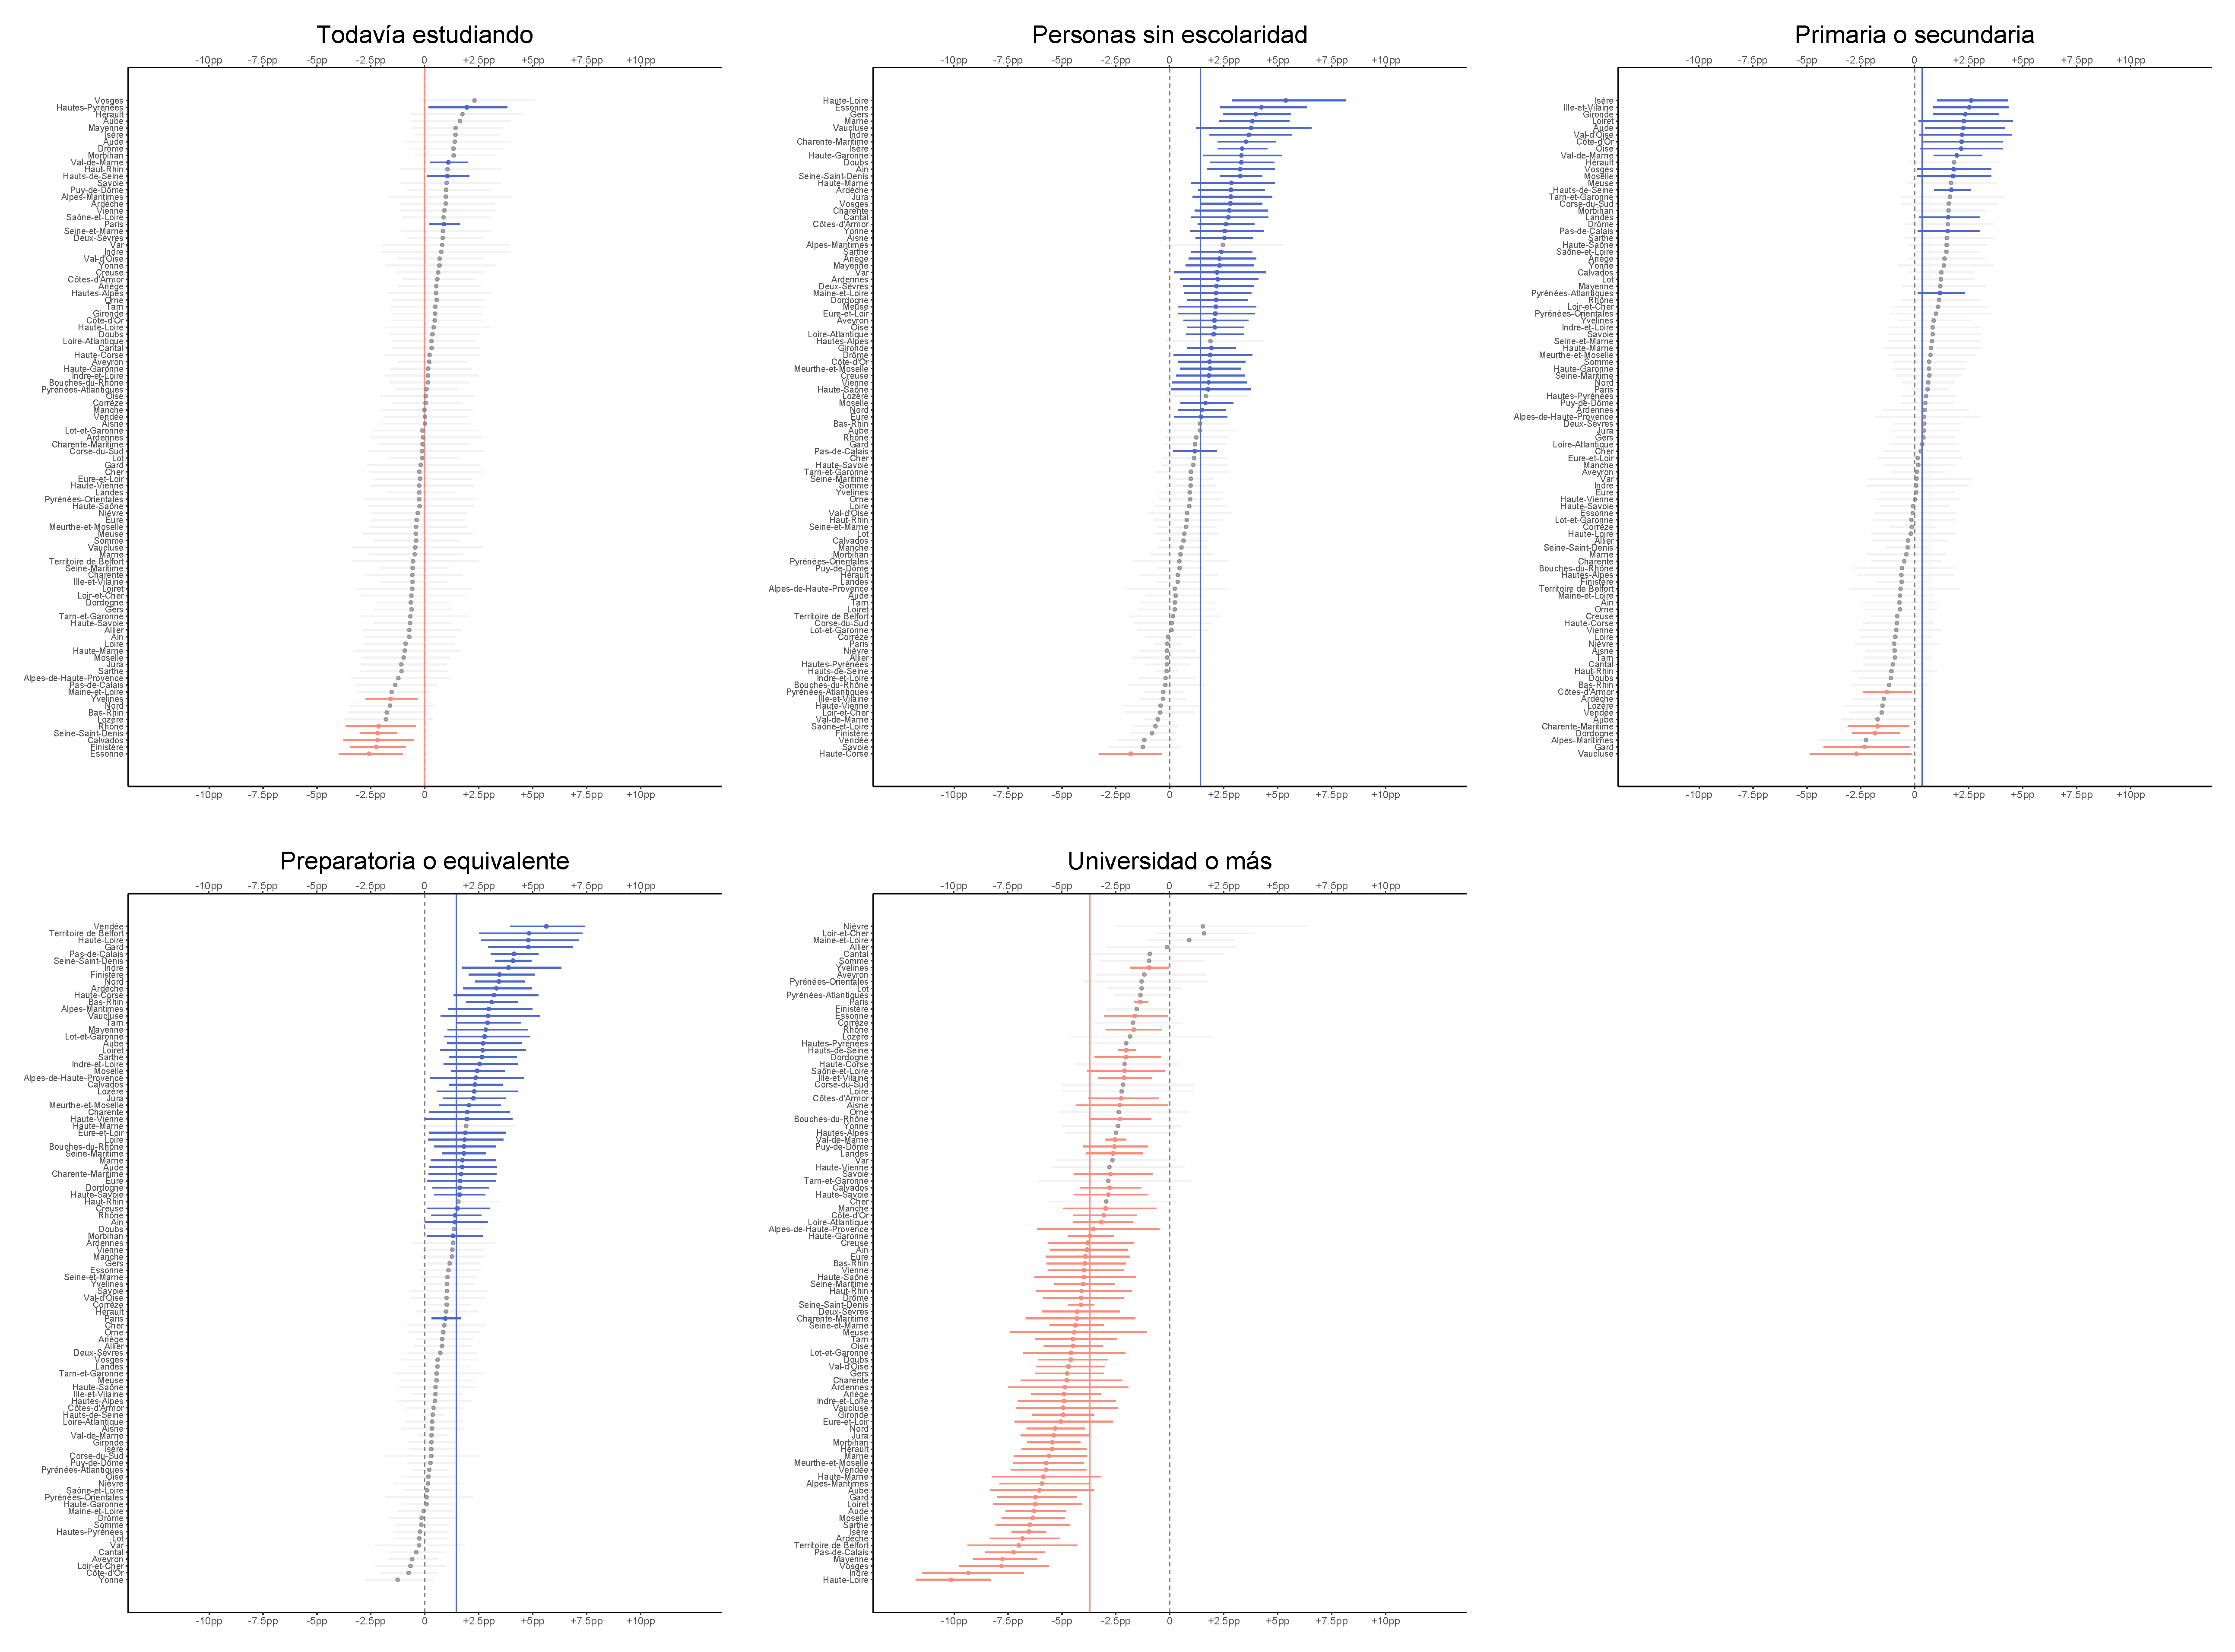
\includegraphics[width = 0.9\textwidth]{Figs/Efectos/Efectos_Escolaridad_Modelo_H}
	\caption{Intervalos centrales de probabilidad al 95\%, 80\% y 50\% para los efectos de la escolaridad por departamento francés bajo el modelo H. Los departamentos se ordenan para cada categoría por magnitud del estimador puntual que es el efecto mediano. Las distribuciones de colores rosa o azul representan que el efecto es significativo al 95\%. Las lineas verticales representan el efecto promedio a través de los departamentos. Fuente: elaboración propia.}
	\label{fig:Efectos_Escolaridad}
\end{figure}

Podemos hacer varias lecturas de este gráfico. En primer lugar confirmamos mediante las líneas verticales que, en general, un aumento en la proporción de personas con estudios universitarios disminuyó la afinidad comunal por Le Pen, de hecho la mayoría de departamentos tienen efectos significativos. Departamentos como Isère y Haute-Loire tienen magnitudes estimadas importantes de casi -4 pp. Por el contrario, el resto de categorías de escolaridad tienen efectos positivos en la afinidad frontista, aunque no todas en la misma magnitud y en todos los departamentos. Confirmamos que para las personas sin escolaridad la mayoría de departamentos tienen un efecto positivo, el más grande de al rededor de 2.5 puntos porcentuales por una desviación estándar de incremento frente a la comuna típica. Pero también vemos que, aunque hay bastante incertidumbre reflejada en la longitud del intervalo, en Haute-Corse el efecto es el contrario, aproximadamente de -1.45 pp.\\ 

La categoría de preparatoria tiene muchos departamentos con efectos significativos positivos y ninguno con efecto significativo negativo. Pero aquí también vemos al modelado jerárquico en acción. Aunque hayan muchos departamentos significativos, la incertidumbre es distinta a través de ellos. Comparemos por ejemplo la longitud de los intervalos de un departamento como Alpes-de-Haute-Provence, el décimo con mayor estimador puntual pero alta incertidumbre, con el de París que es el de menor magnitud entre los significativos y sobre el que no tenemos prácticamente nada de incertidumbre. También podemos ver en el caso de las personas que todavía estudian que pueden existir efectos con un estimador puntual mayor al de otros, pero que no son significativos.\\

\begin{figure}[h]
	\centering
	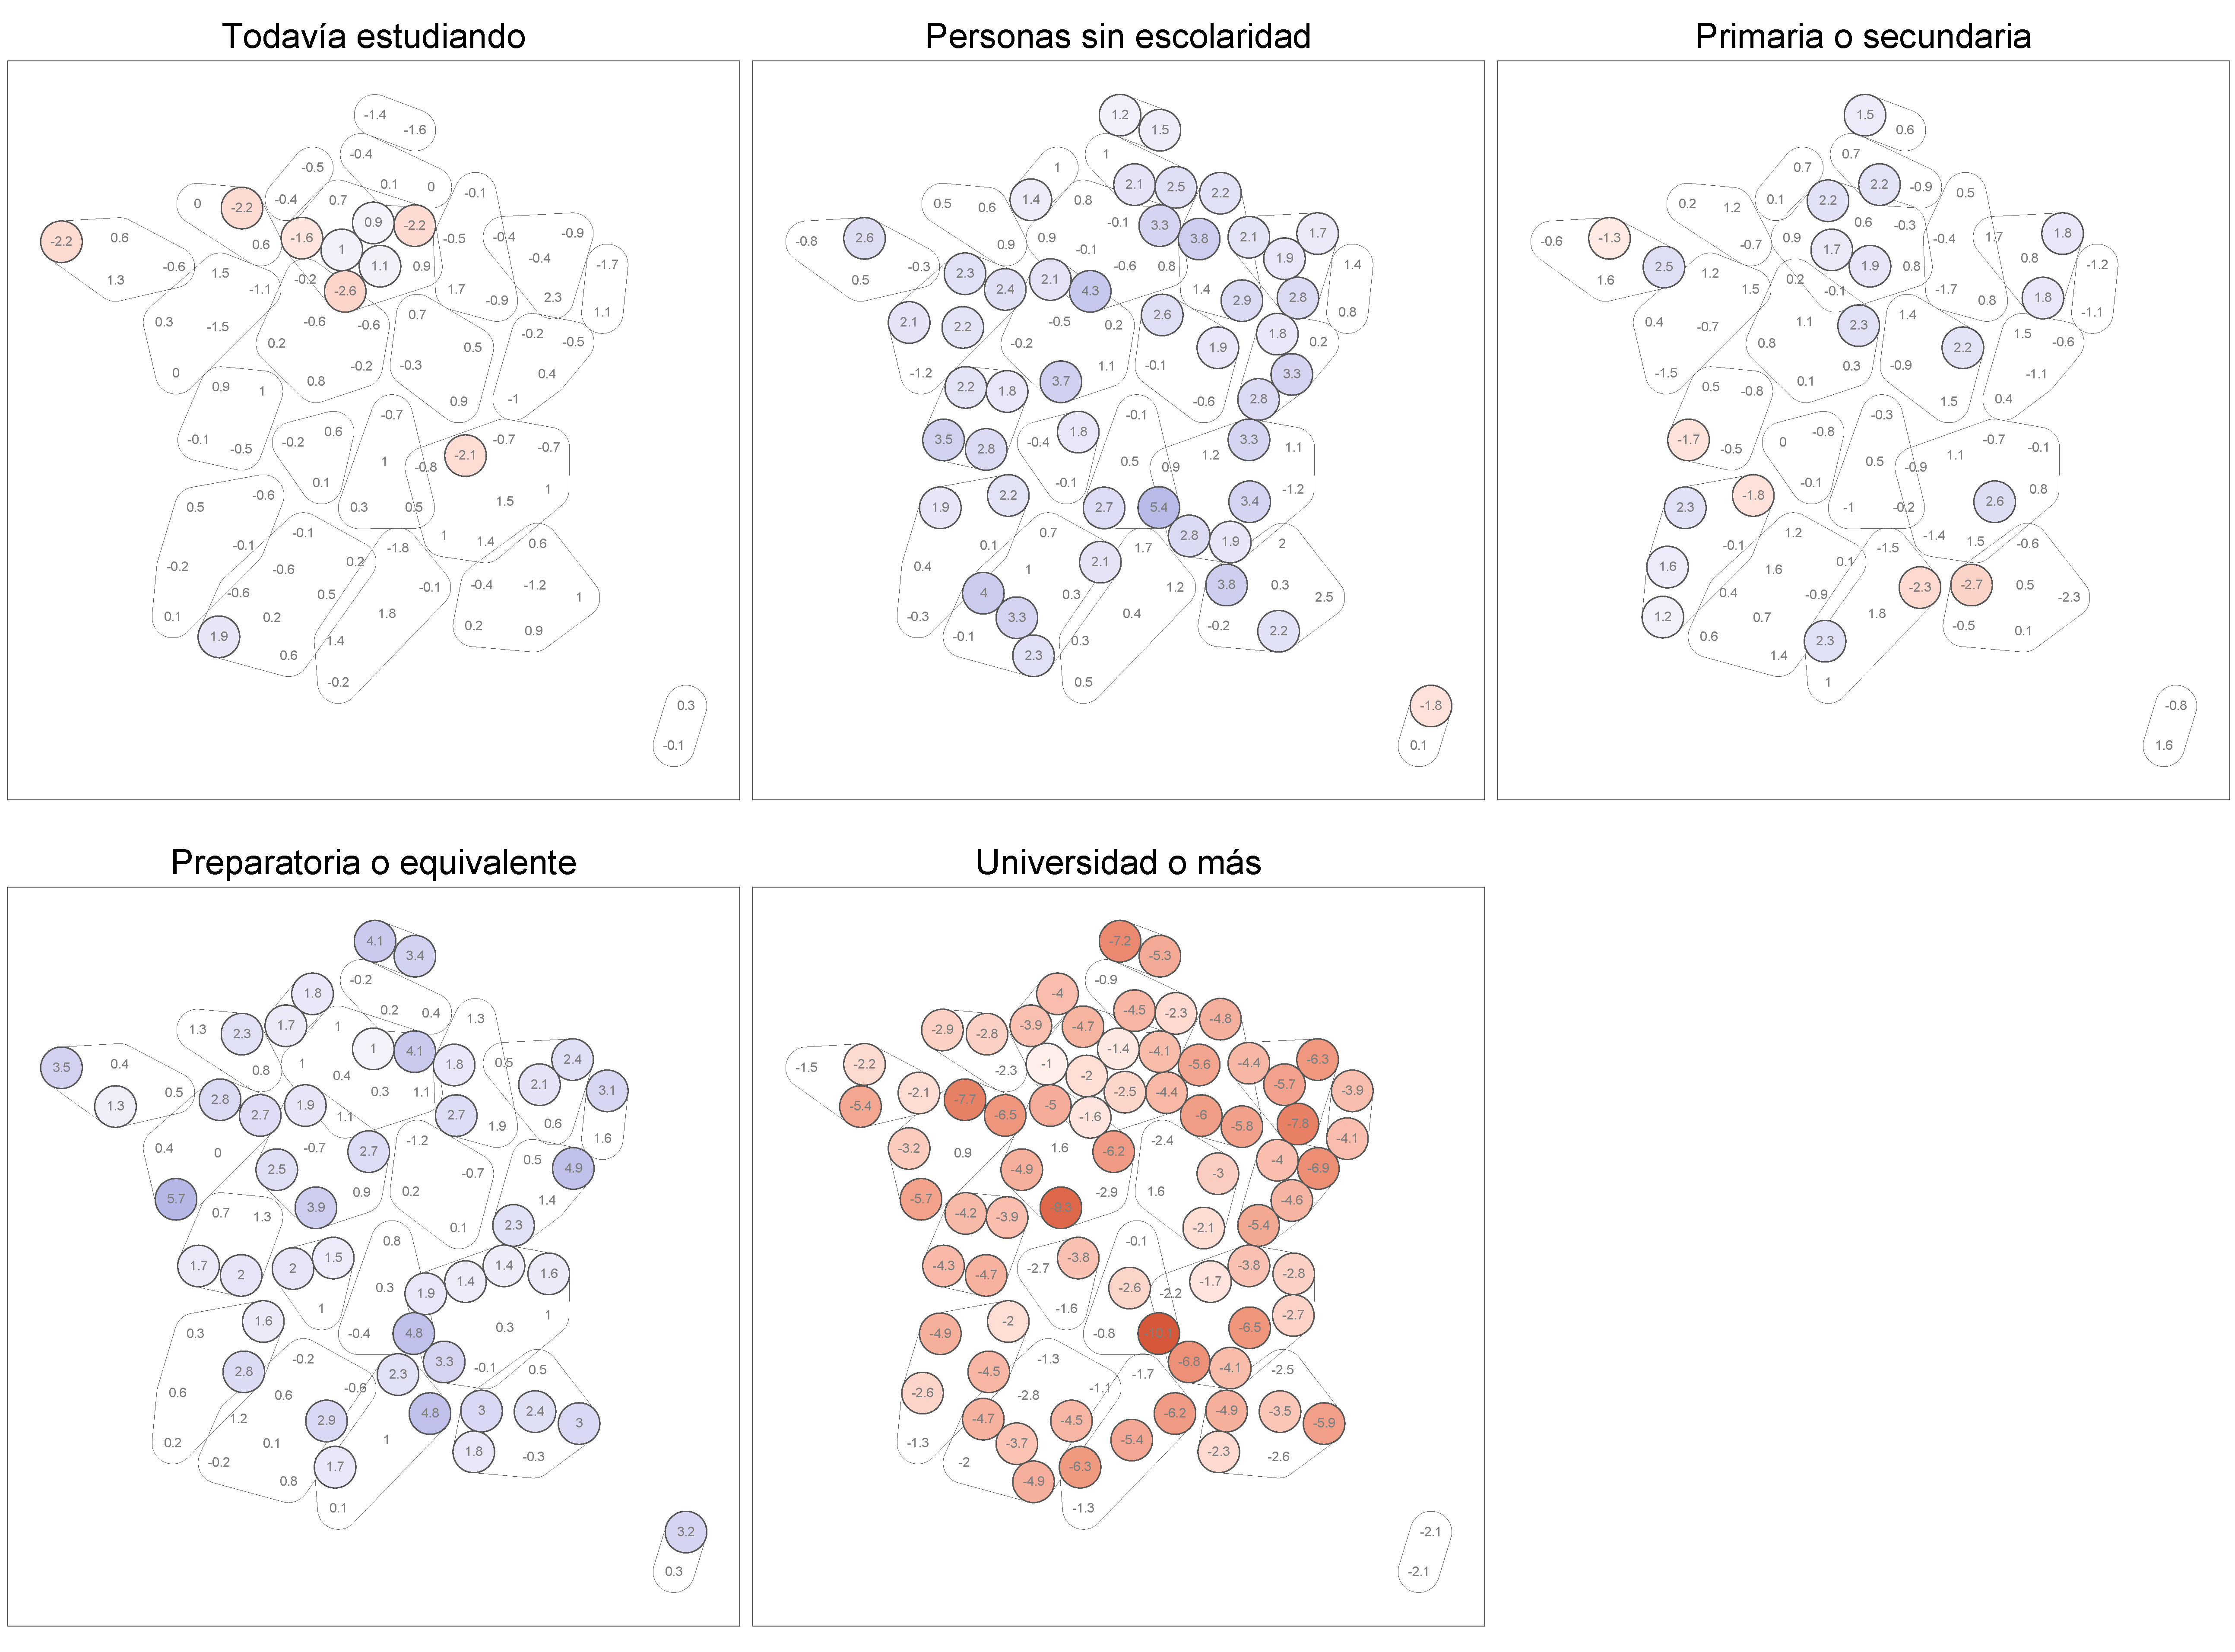
\includegraphics[width = 0.9\textwidth]{Figs/Efectos/Dorling_Efectos_Escolaridad_Modelo_H}
	\caption{Estimaciones puntuales de los efectos de la escolaridad por departamento francés bajo el modelo H, solo se colorean los efectos significativos. Fuente: elaboración propia.}
	\label{fig:Dorling_Efectos_Escolaridad}
\end{figure}

Tomando en cuenta entonces el carácter de significancia o no de un efecto, podemos modificar el mapa de la \textbf{Figura \ref{fig:Mapa_Efectos_Escolaridad}} y convertirlo en el dorling de la \textbf{Figura \ref{fig:Dorling_Efectos_Escolaridad}}. En este último, solo tienen color los departamentos con efecto significativo, aunque reporto los efectos esperados en todos los departamentos. Aquí identificamos que las únicas zonas donde el efecto de los universitarios no parece ser significativo es en departamentos más rurales como el llamado \textit{Massif Central}. Por el contrario, si en general el porcentaje de personas que todavía estudian no parecía ser tan importante, aquí observamos que sus efectos significativos se concentran en la región de Île de France. 

\subsection{Categorías socioprofesionales}

La segunda variable a considerar son las categorías socioprofesionales. Como indicaba en la revisión de literatura esta es probablemente la variable más utilizada en el estudio de la sociología electoral francesa. A pesar de ello, los mapas de la \textbf{Figura \ref{fig:Mapa_Efectos_Cat_Socioprof}} aparecen descolorados para la mayoría de categorías, indicando efectos muy pequeños. Resalta inmediatamente un departamento al noreste francés coloreado con un azul más intenso en el panel de obreros, la que es la categoría que parece tener una mayor asociación positiva con las preferencias por Marine Le Pen. Esto refuerza las hipótesis sobre \textit{gaucho-lépénisme} discutidas en la primera parte de este trabajo. Llama particularmente la atención la falta de intensidad en los efectos de los artesanos, comerciantes y empresarios, un grupo tradicionalmente asociado al FN. Otro punto interesante es notar que los cuadros y las profesiones intelectuales superiores tienen un efecto negativo, salvo en pocos departamentos que aparecen claramente en azul.\\ 

\begin{figure}[h]
	\centering
	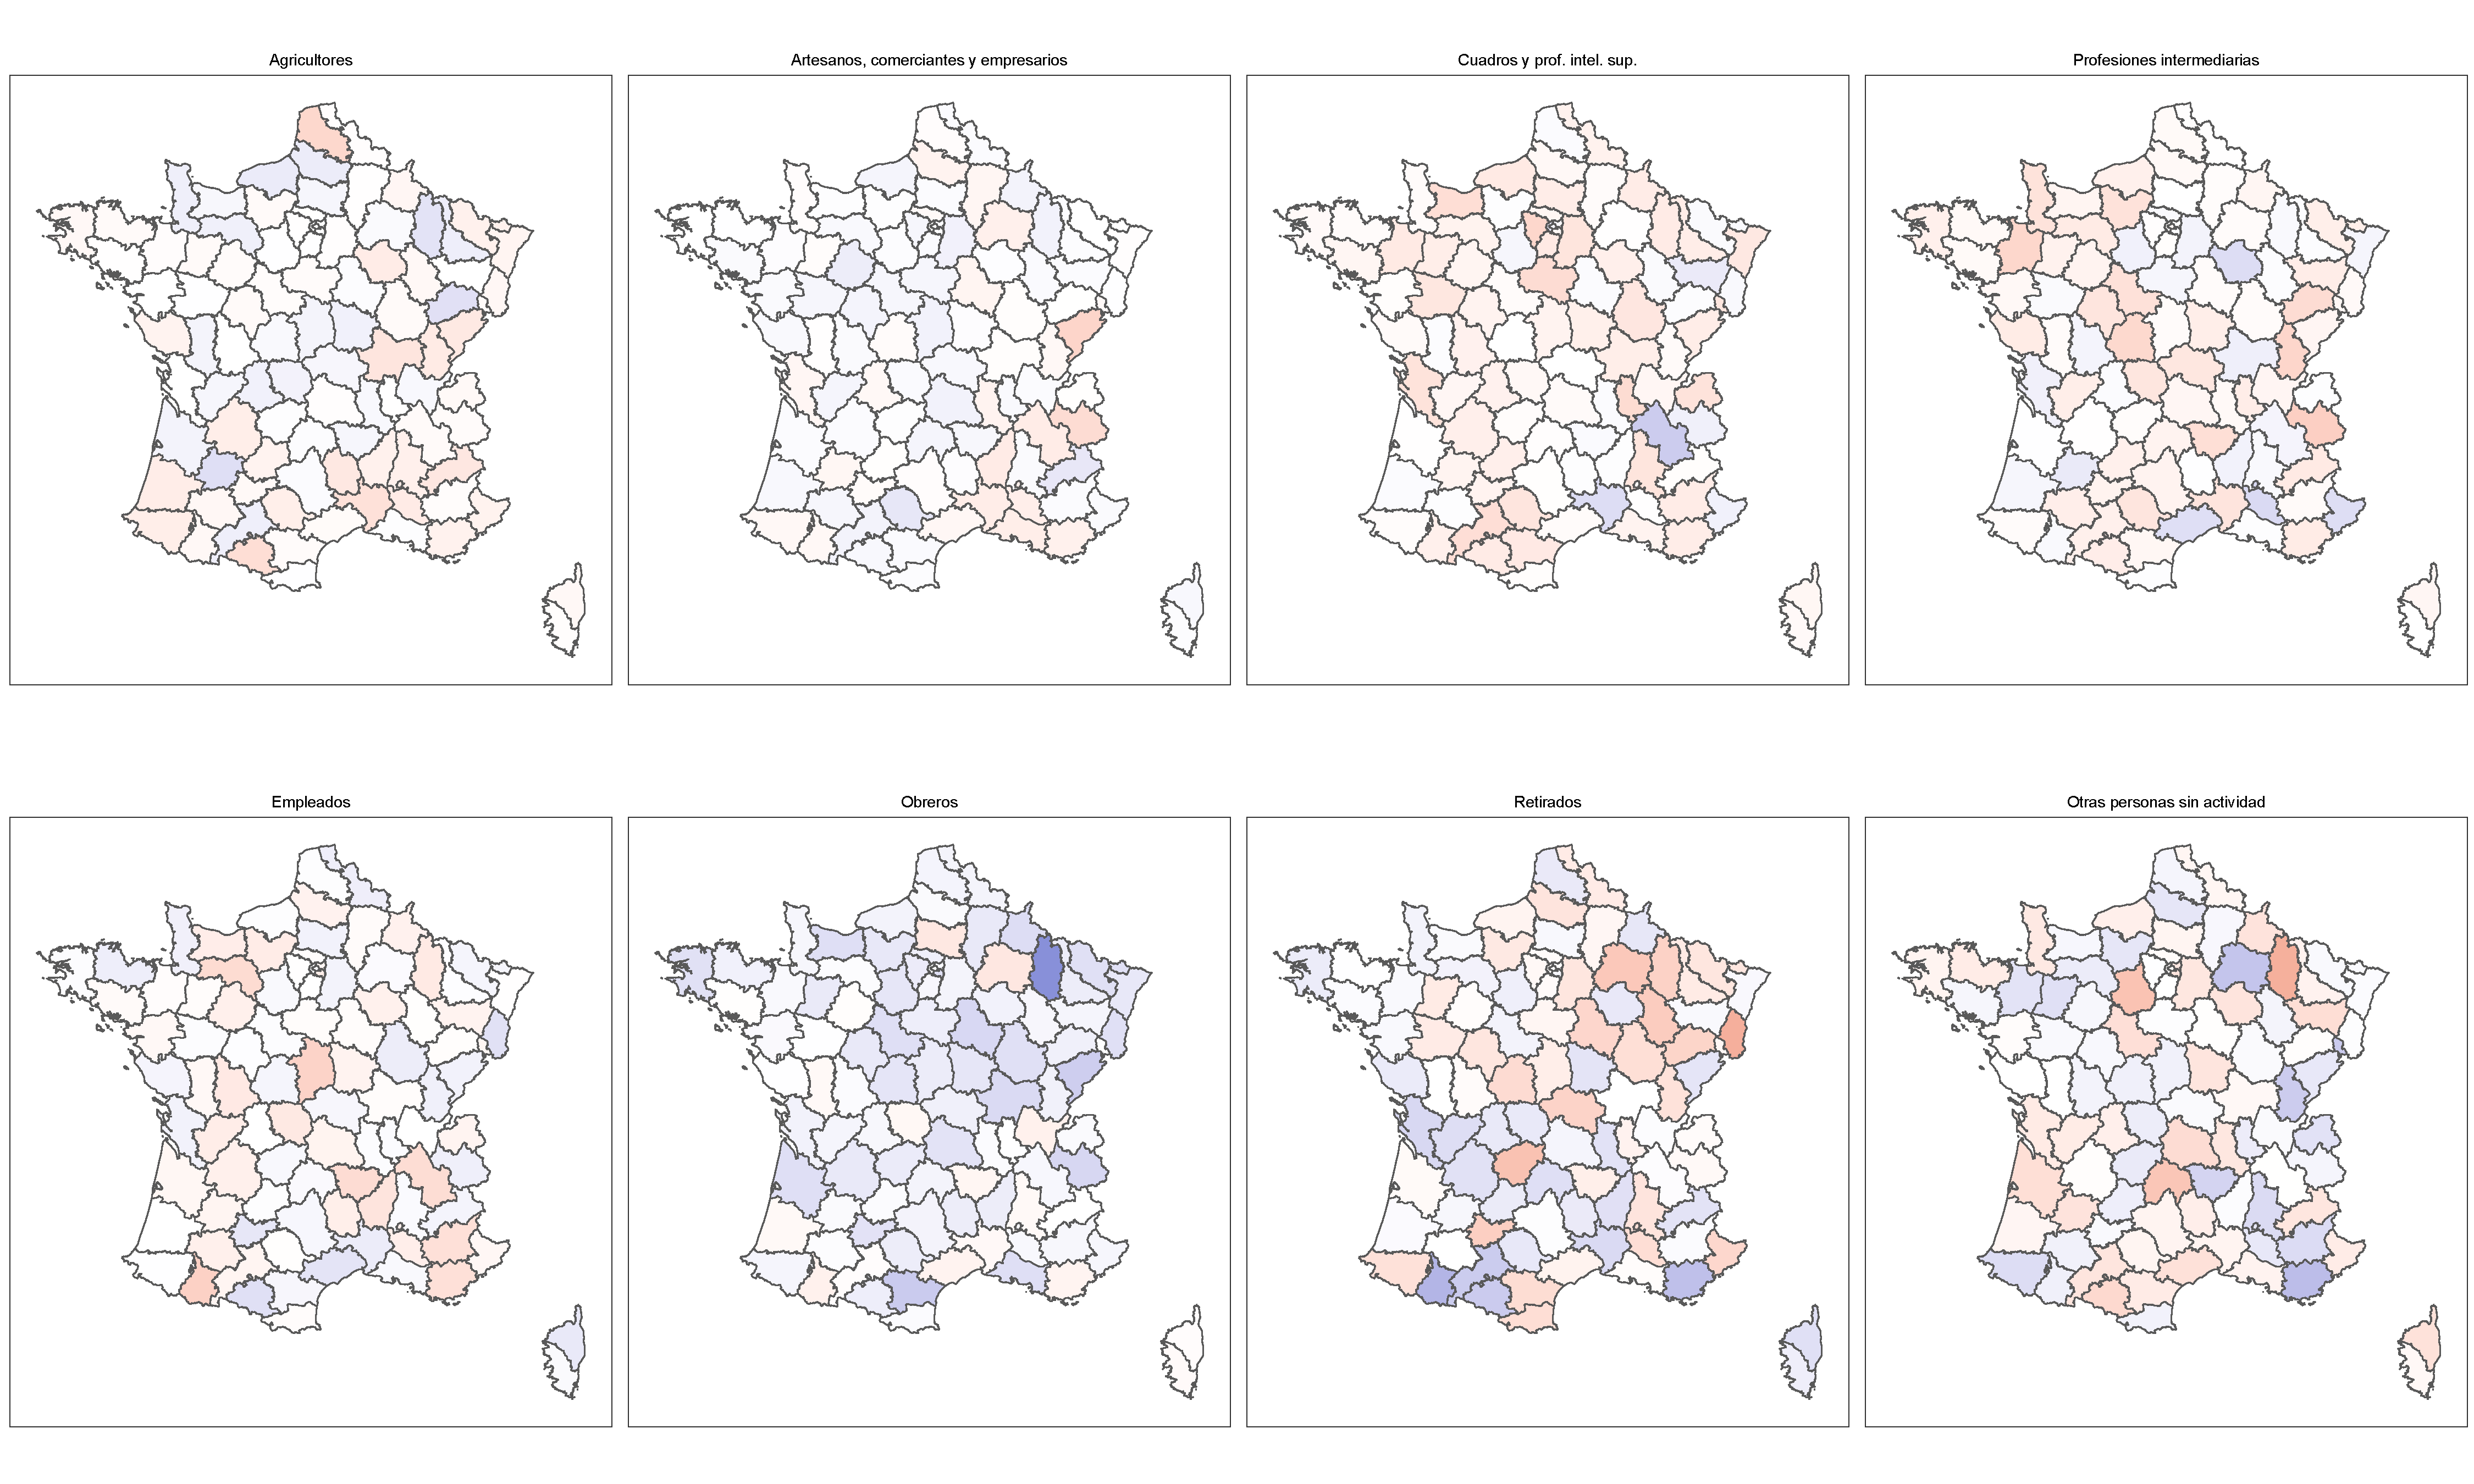
\includegraphics[width = 0.9\textwidth]{Figs/Efectos/Mapa_Efectos_Cat_Socioprof_Modelo_H}
	\caption{Estimaciones puntuales de los efectos de la categoría socioprofesional por departamento francés bajo el modelo H. Fuente: elaboración propia con la cartografía de Open Street Map.}
	\label{fig:Mapa_Efectos_Cat_Socioprof}
\end{figure}

Al observar los intervalos de los efectos en la \textbf{Figura \ref{fig:Efectos_Cat_Socioprof}}, confirmamos que la mayoría de las categorías tienen efectos muy pequeños de acuerdo a los promedios a través de departamentos observados en las líneas verticales. La única categoría con un efecto promedio mayor parece ser la de los obreros donde Meuse es el departamento con el mayor efecto, de más de 4 puntos porcentuales. Esta también sería la categoría socioprofesional más cercana a un sentimiento de clase lo que podría explicar su mayor homogeneidad nacional frente a otras categorías que, como la investigación de \textcite{MayerMichelat81} ya sugería, pueden cambiar más sus inclinaciones políticas dependiendo del contexto local, reafirmando incluso la influencia que la mayor presencia de obreros tiene en la preferencia electoral de otras categorías.\\ 

Llama la atención también que para las profesiones intermediarias la mayoría de los efectos significativos son negativos, sin embargo tenemos 4 departamentos con claros efectos positivos y todos en zonas de fortaleza del FN: Vaucluse, Alpes-Maritimes y Hérault en el litoral mediterráneo y Aube en el noreste francés. El caso de los retirados es interesante porque si bien la mayoría de los efectos son nulos, hay algunos significativos tanto positivos como negativos y la gráfica se ve más dispersa. Este es un ejemplo donde el modelo jerárquico se asemeja más a un modelo de no agregación o regresiones independientes. Por el contrario, las gráficas en la que las curvas son casi verticales, indicando efectos muy parecidos para todos los departamentos, serían casos más parecidos a los modelos de agregación completa o una sola regresión nacional.\\ 

\begin{figure}[h]
	\centering
	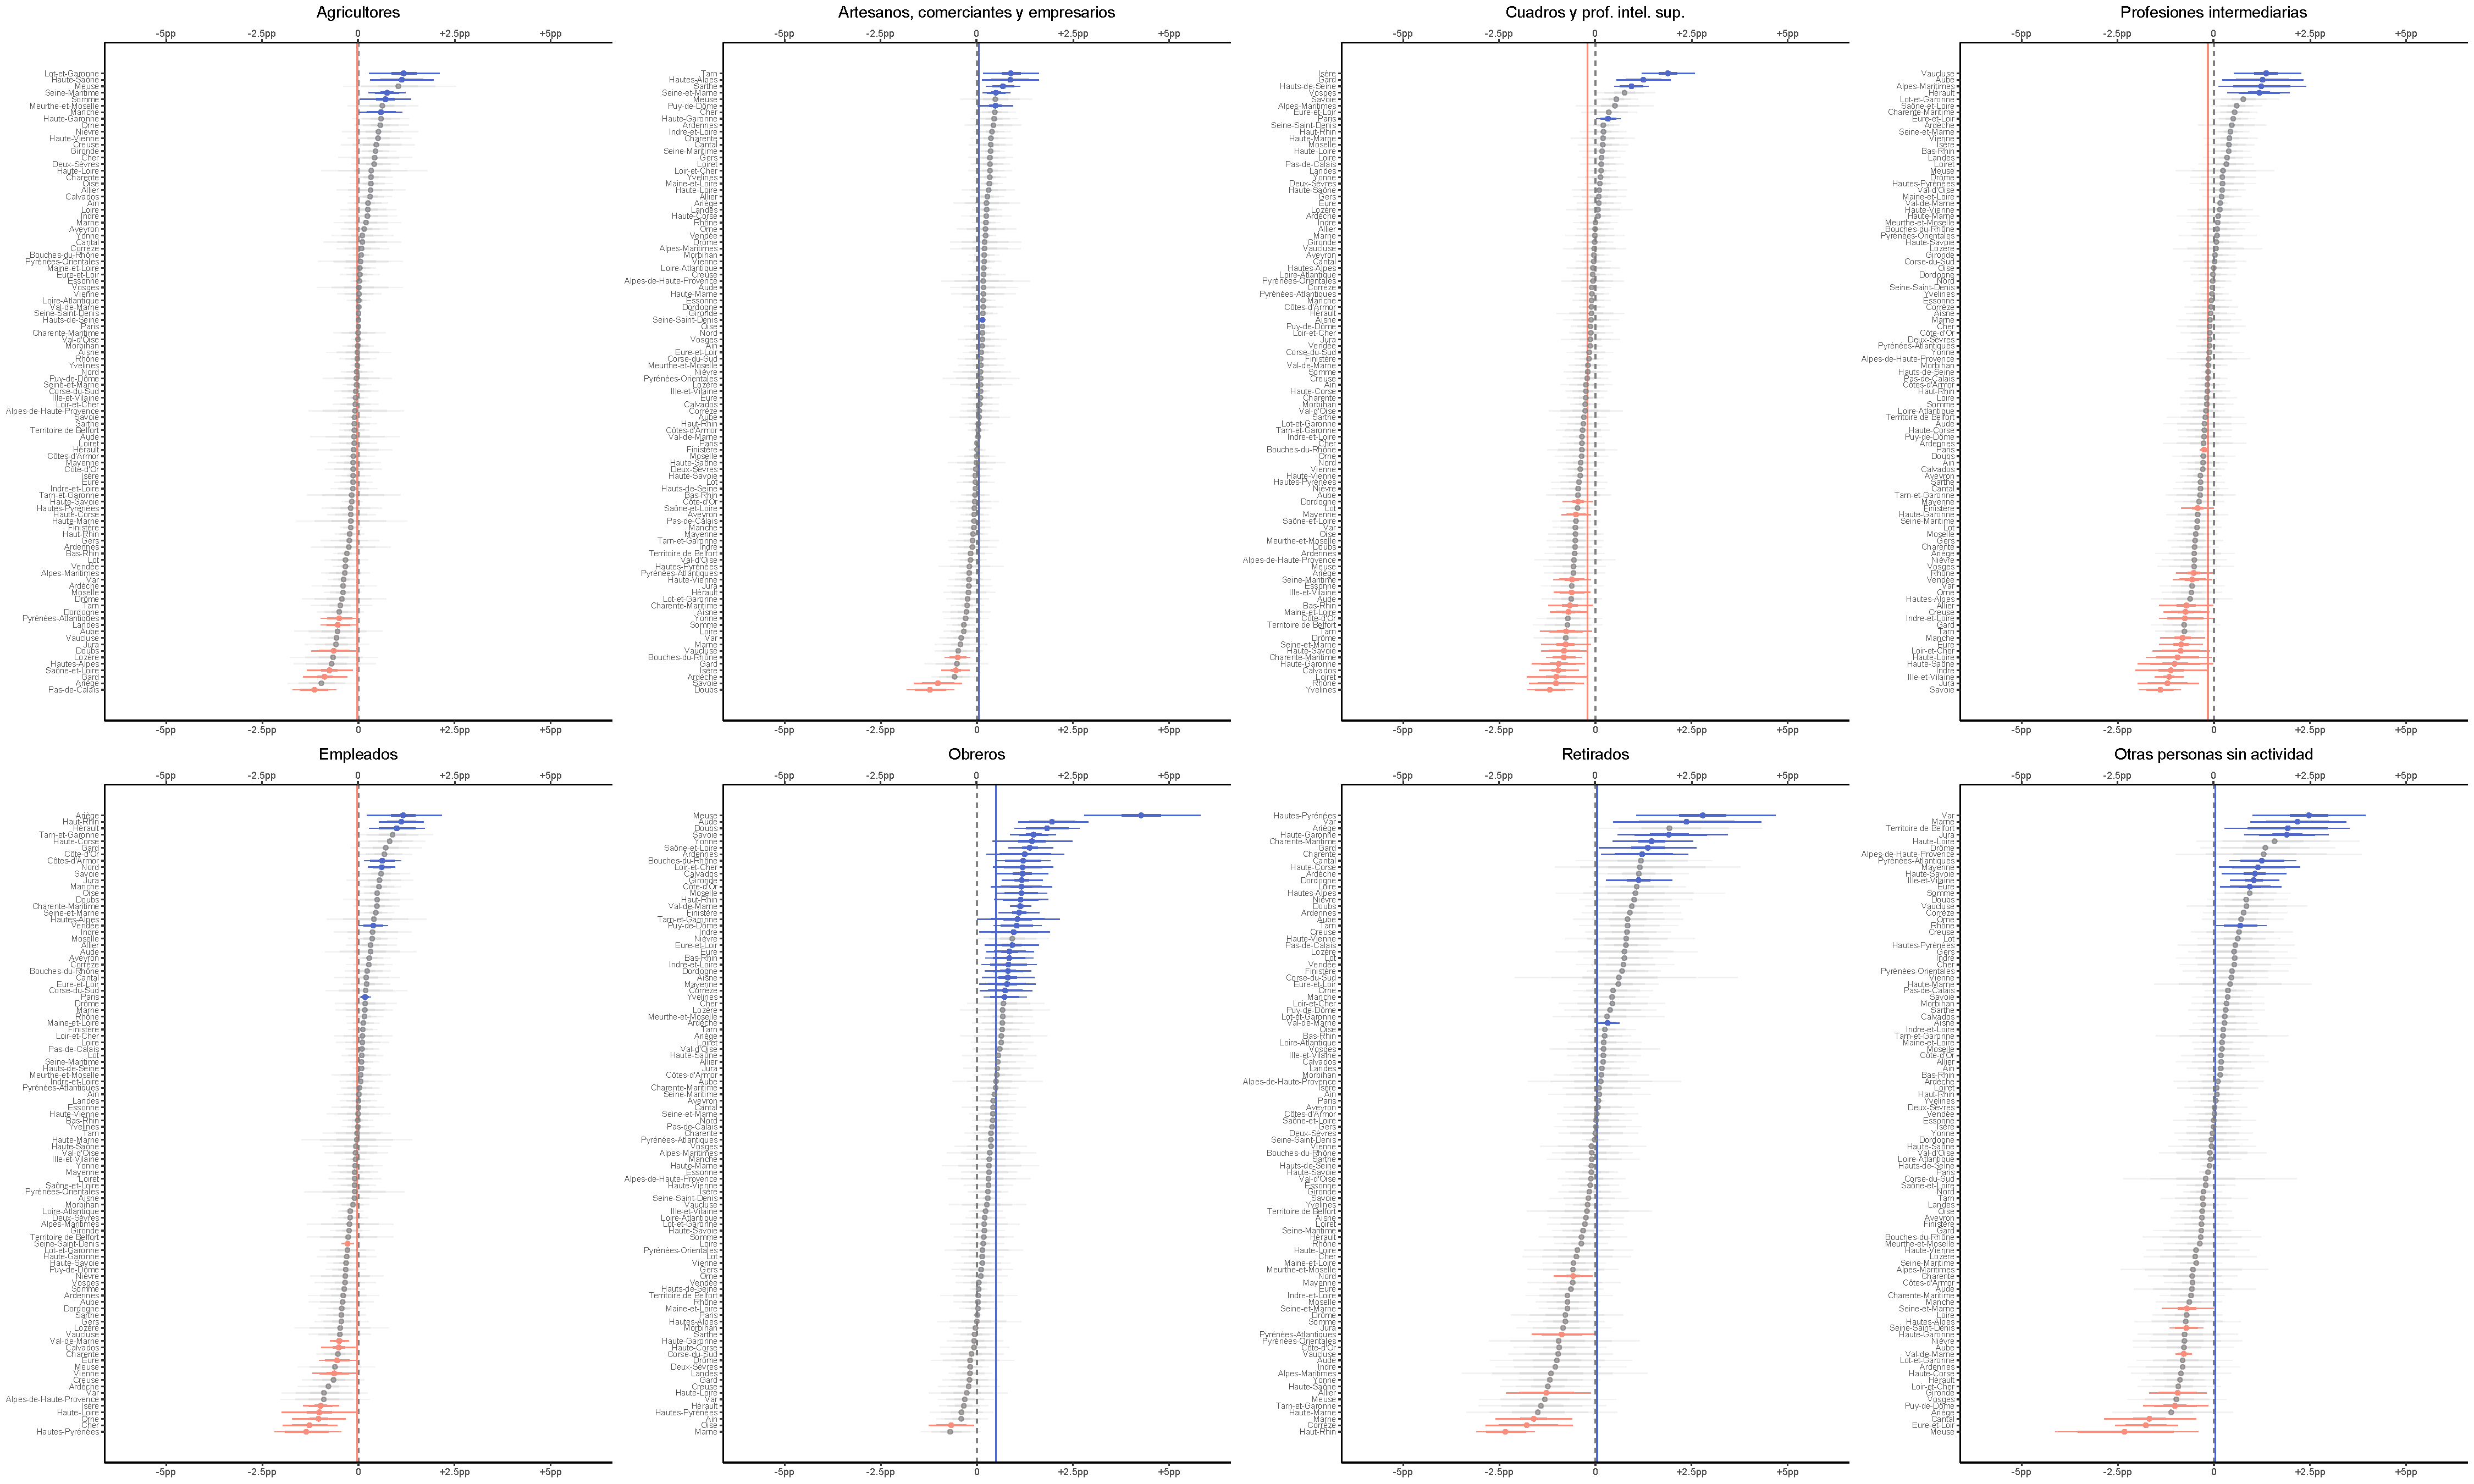
\includegraphics[width = 0.9\textwidth]{Figs/Efectos/Efectos_Cat_Socioprof_Modelo_H}
	\caption{Intervalos centrales de probabilidad al 95\%, 80\% y 50\% para los efectos de la categoría socioprofesional por departamento francés bajo el modelo H. Los departamentos se ordenan para cada categoría por magnitud del estimador puntual que es el efecto mediano. Las distribuciones de colores rosa o azul representan que el efecto es significativo al 95\%. Las lineas verticales representan el efecto promedio a través de los departamentos. Fuente: elaboración propia.}
	\label{fig:Efectos_Cat_Socioprof}
\end{figure}

La geografía de los efectos significativos que se observa en los dorlings de la \textbf{Figura \ref{fig:Dorling_Efectos_Cat_Socioprof}} tiene algunos puntos notables. El norte más industrializado se asocia con mayores efectos de la clase obrera. Vemos la particularidad del litoral mediterráneo en términos de profesiones intermediarias. Quizás sorprende que en París una mayor presencia de cuadros lleva a una mayor preferencia frontista. La explicación podría estar en que los cuadros que logran vivir dentro de París tiendan a ser más cercanos a la derecha, pero esta tendría que ser una hipótesis a explorarse con mayor detalle en otro tipo de estudio.\\ 

\begin{figure}[h]
	\centering
	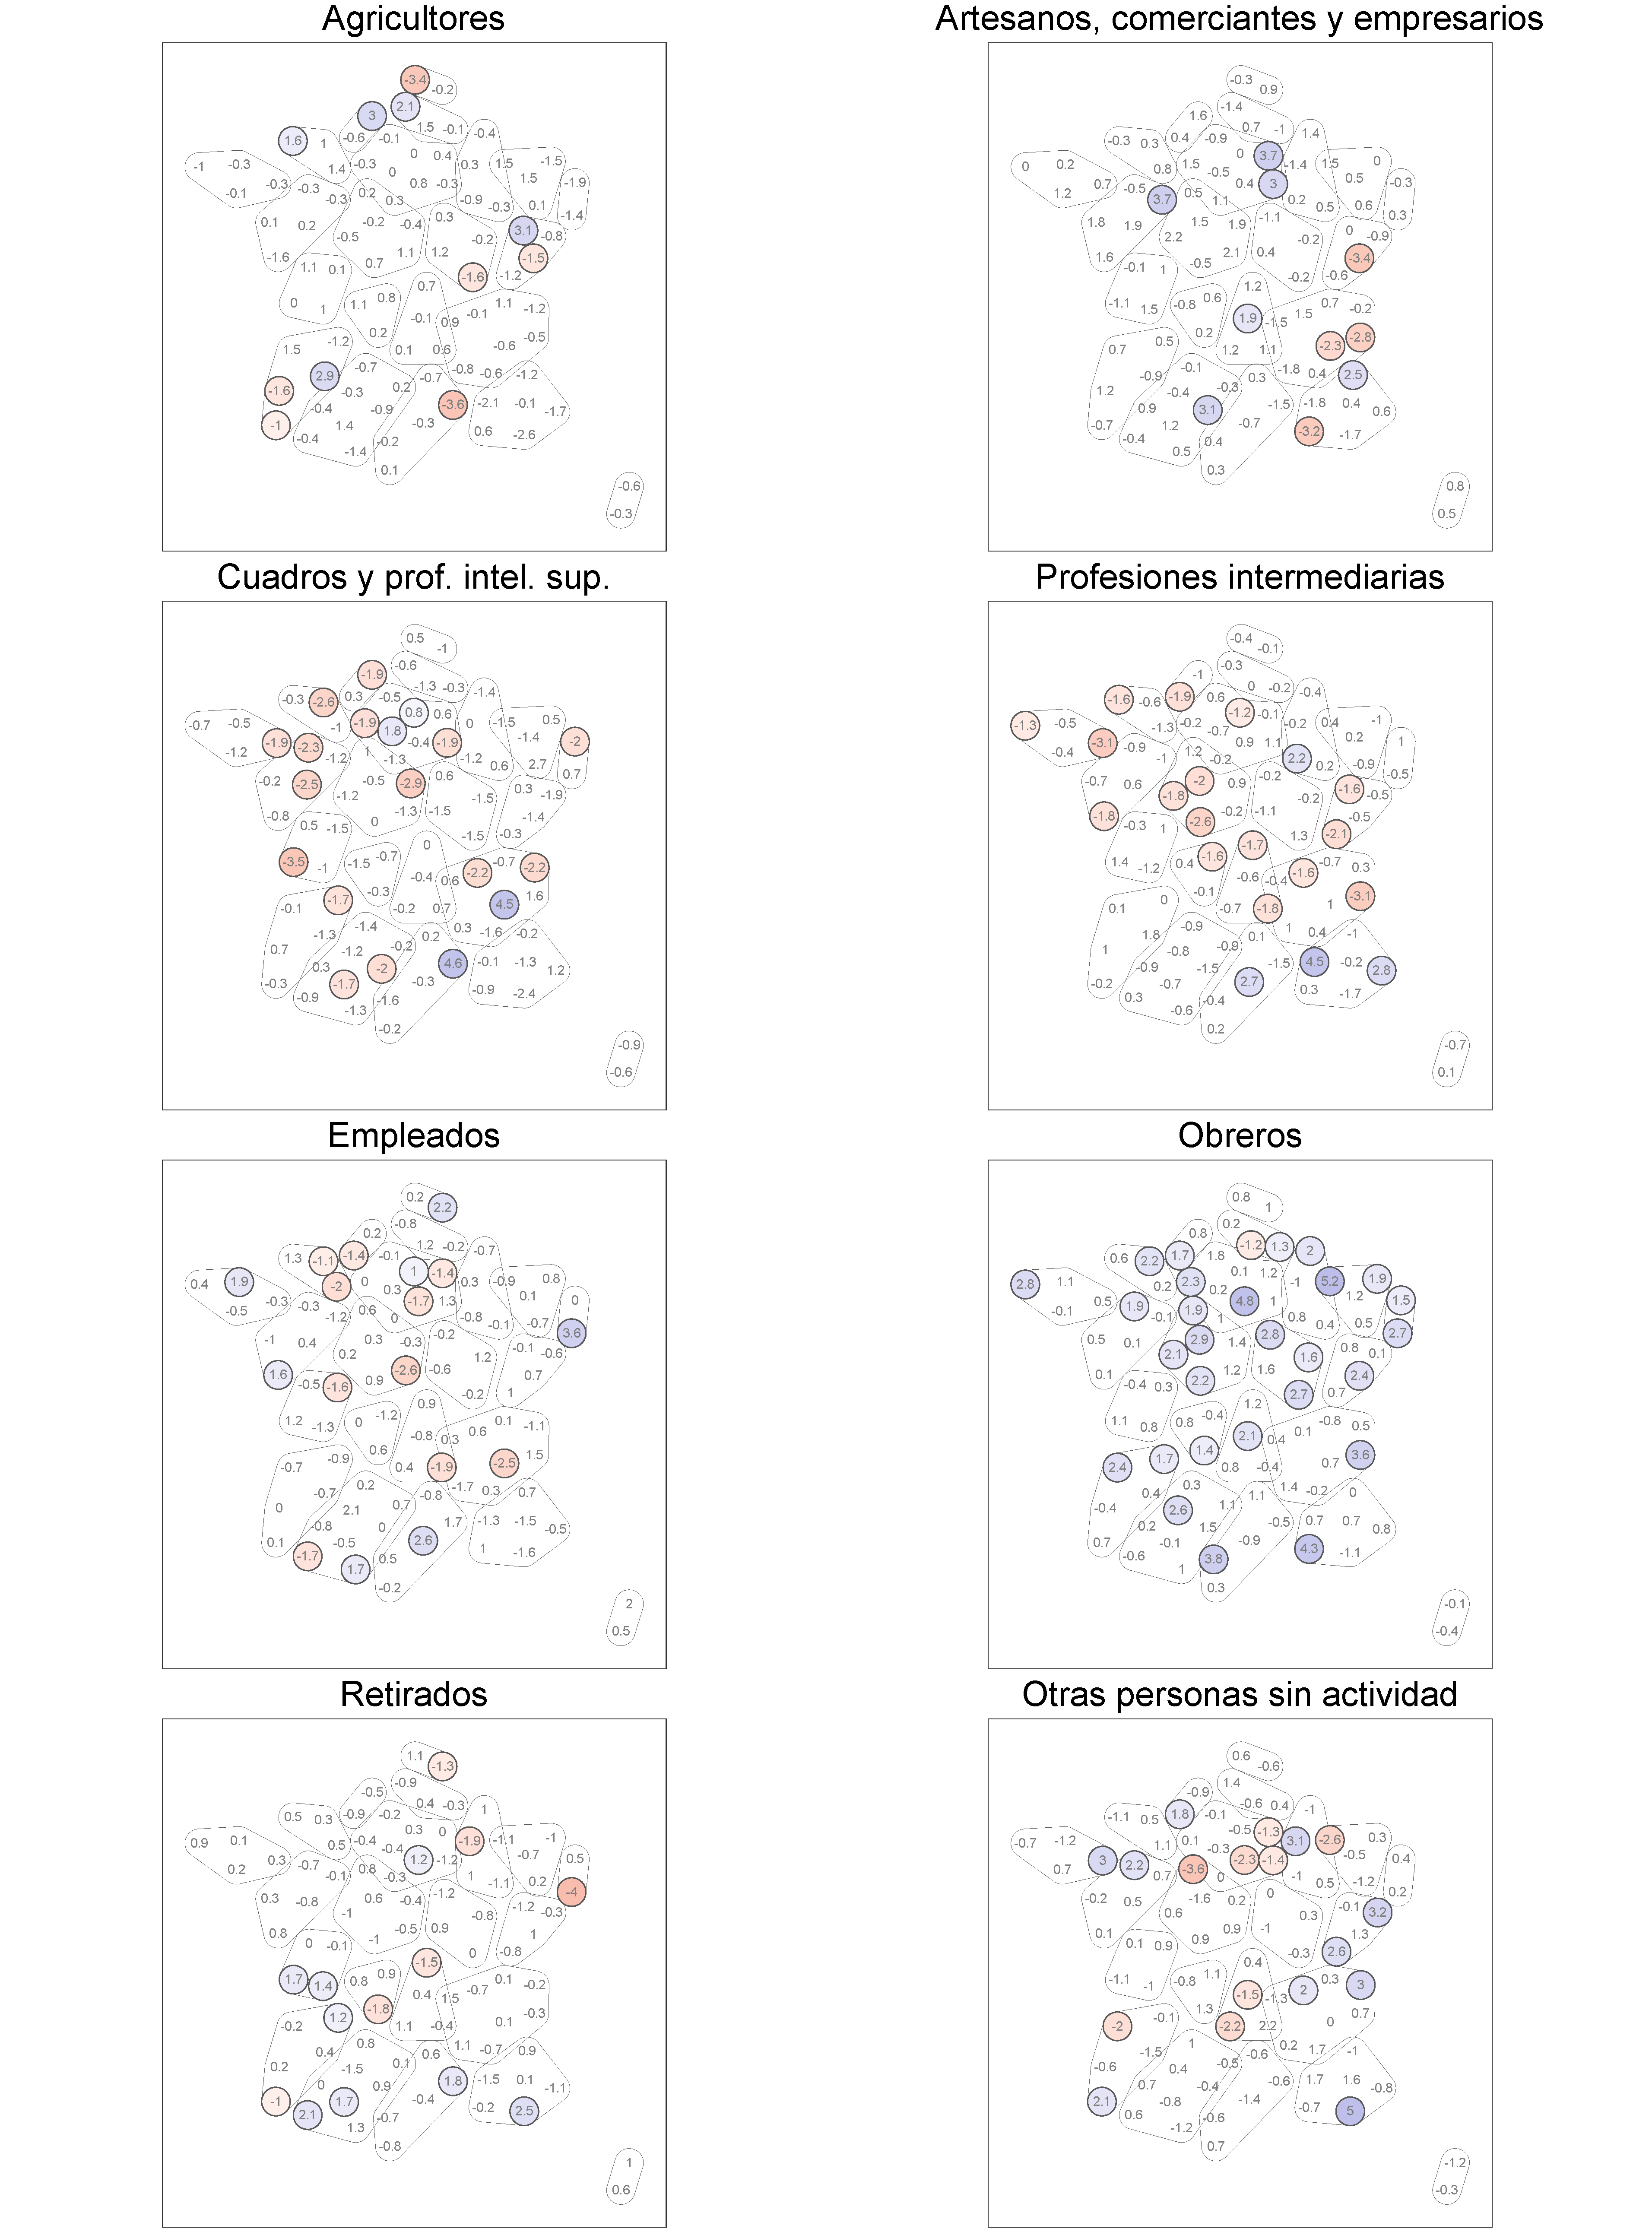
\includegraphics[width = 0.9\textwidth]{Figs/Efectos/Dorling_Efectos_Cat_Socioprof_Modelo_H}
	\caption{Estimaciones puntuales de los efectos de la categoría socioprofesional por departamento francés bajo el modelo H, solo se colorean los efectos significativos. Fuente: elaboración propia.}
	\label{fig:Dorling_Efectos_Cat_Socioprof}
\end{figure}

\subsection{Edad}

Las explicaciones culturalistas, principalmente las de la escuela de Inglehart, hablan de que las generaciones de edad crecen con ciertos valores que los llevan a tener determinadas posiciones políticas. En este sentido podríamos leer los mapas de la \textbf{Figura \ref{fig:Mapa_Efectos_Edad}} como reflejo de los valores generacionales, lo que explicaría la mayor homogeneidad frente a las variables antes analizadas. La mayor presencia de adultos mayores estaría relacionada negativamente con el FN porque este grupo de edad tiene una simpatía por la derecha tradicional. Los jóvenes de entre 18 a 24 años, por el contrario, tendrían posiciones políticas contrarias al carácter NAP del FN. La asociación positiva con los menores de edad podría reflejar un efecto cultural en comunas con altas tasas de natalidad o menos avejentadas. Esta hipótesis podría también explicar por qué los departamentos que parecen tener la tendencia contraria son aquelos de Île de France: la mayor presencia de inmigrantes, que normalmente tienen mayores tasas de natalidad, frenaría el voto nativista que los rechaza. Tendríamos que confirmar esto al analizar el efecto que los inmigrantes tuvieron según el modelo.\\

\begin{figure}[h]
	\centering
	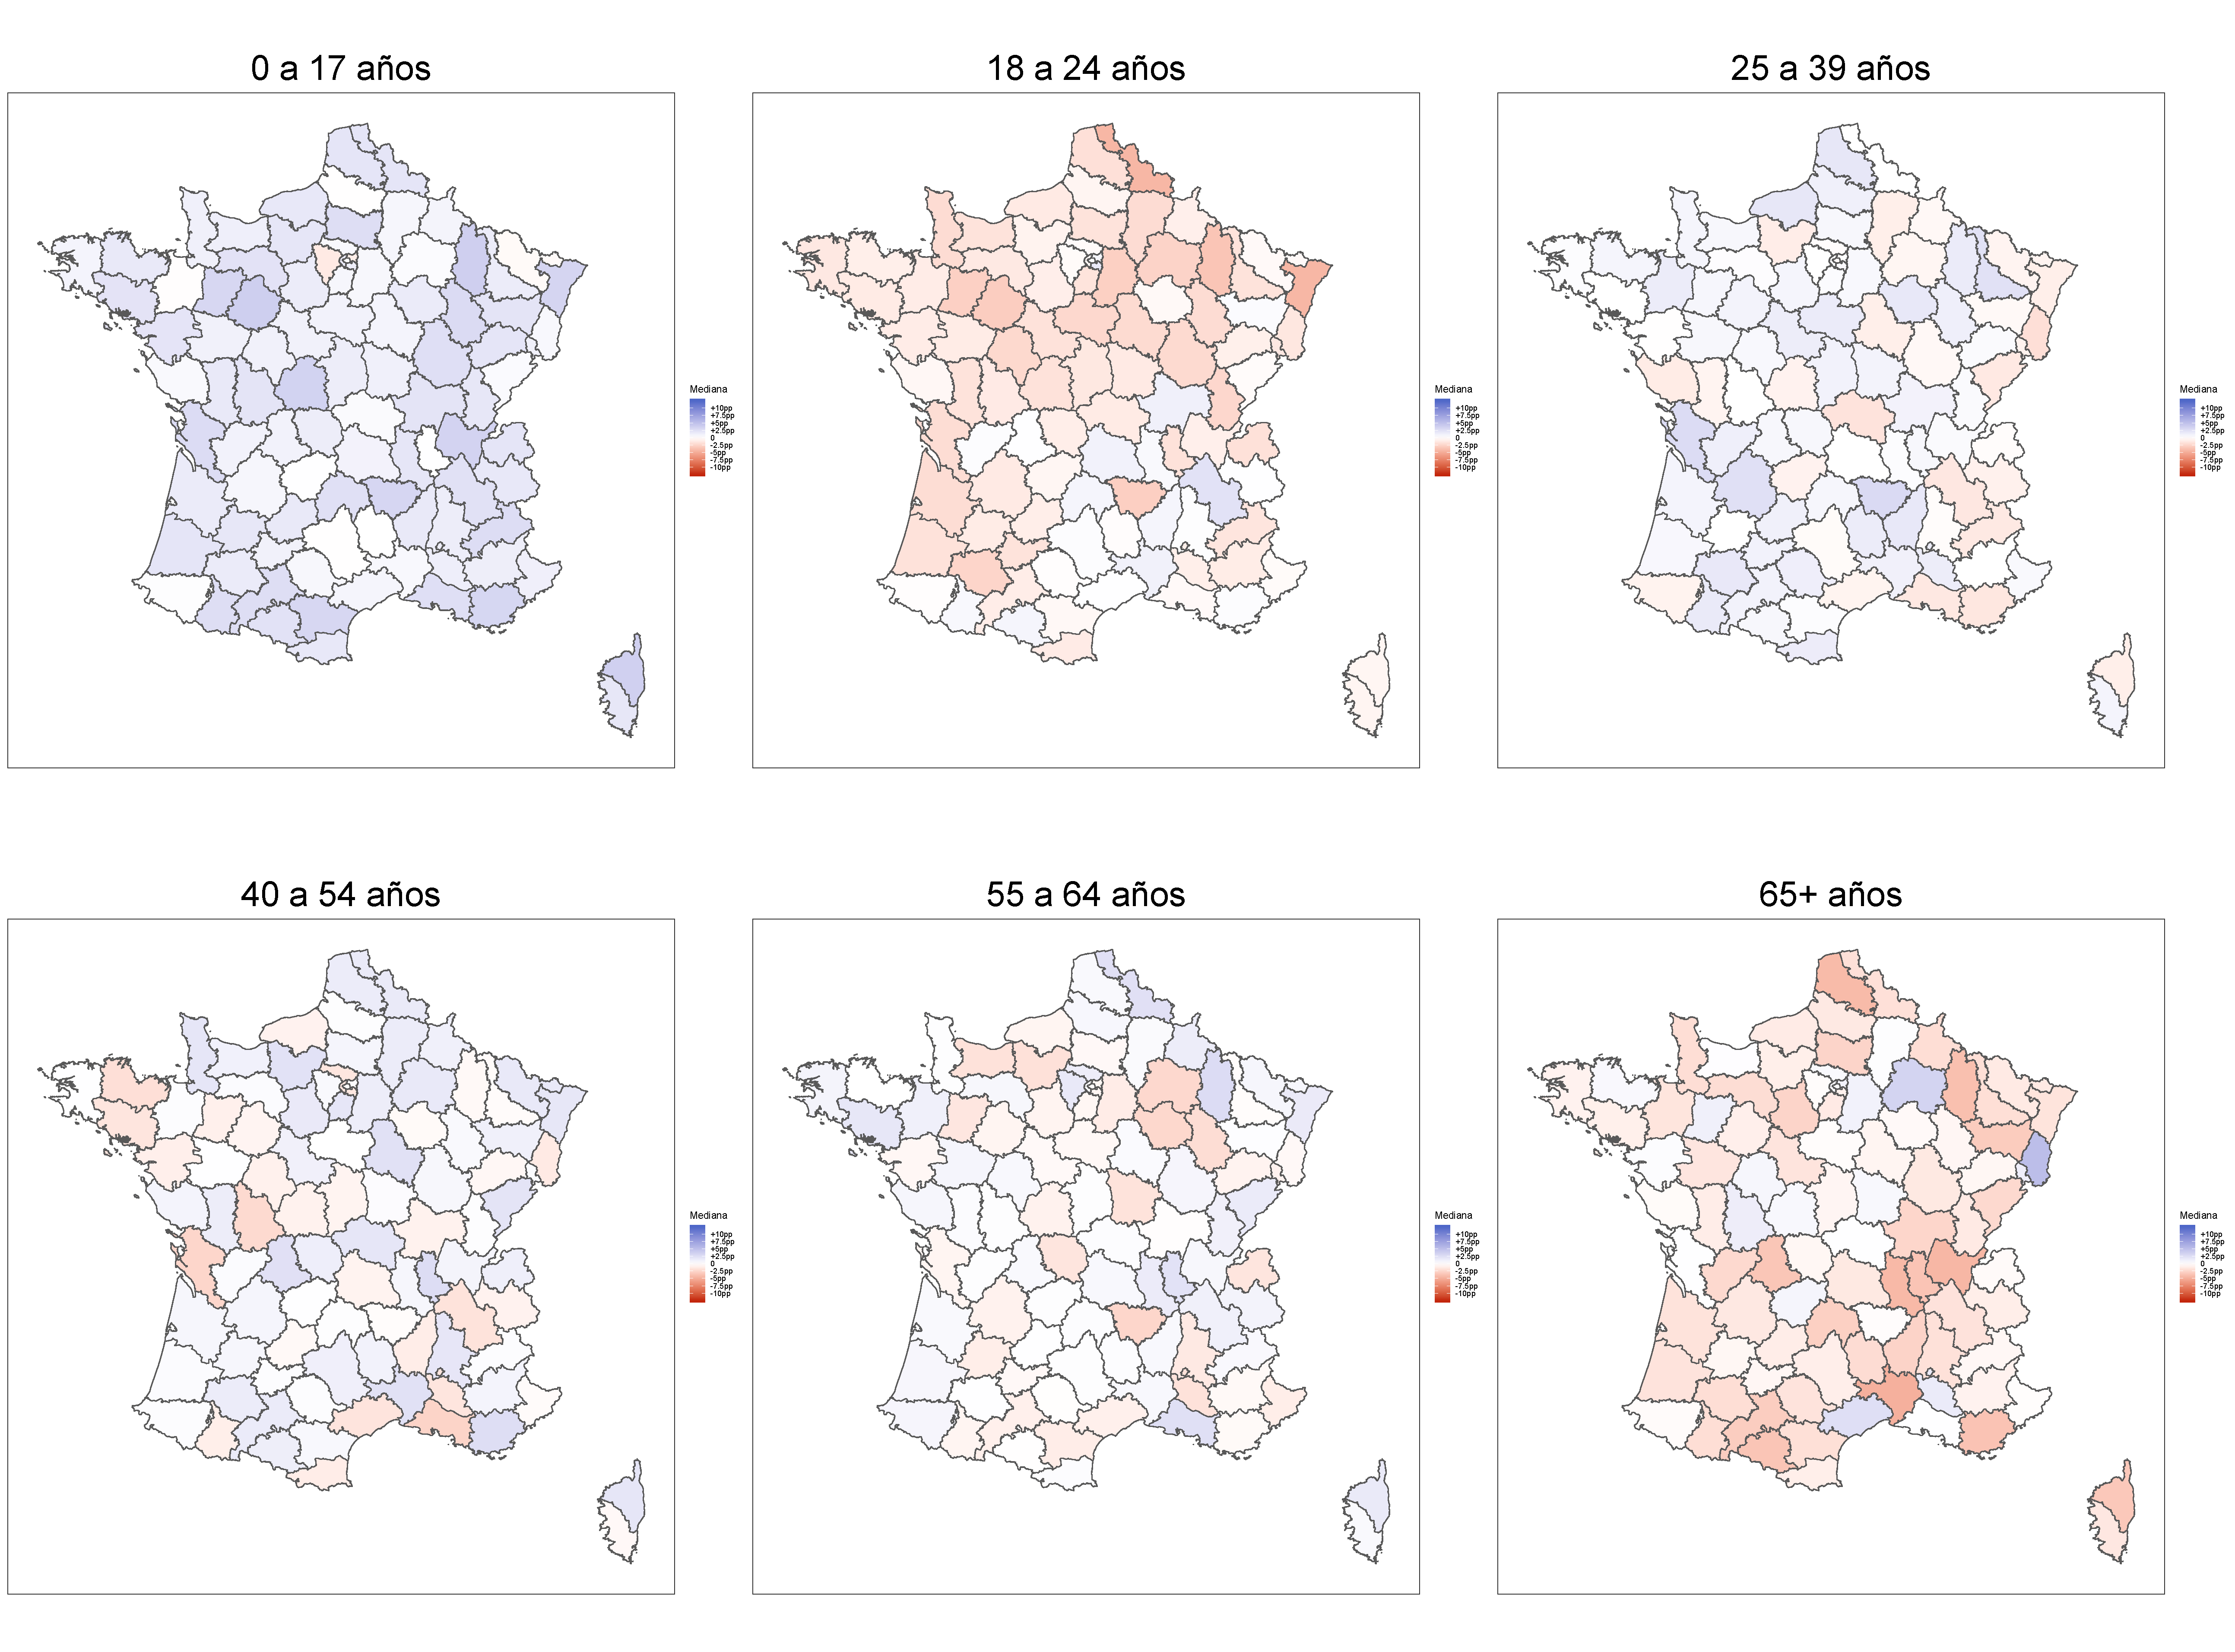
\includegraphics[width = 0.9\textwidth]{Figs/Efectos/Mapa_Efectos_Edad_Modelo_H}
	\caption{Estimaciones puntuales de los efectos del grupo de edad por departamento francés bajo el modelo H. Fuente: elaboración propia con la cartografía de Open Street Map.}
	\label{fig:Mapa_Efectos_Edad}
\end{figure}

Al observar los resúmenes distribucionales confirmamos que los menores de edad y los adultos mayores son los grupos de edad que tienen mayor variabilidad e incertidumbre. En la \textbf{Figura \ref{fig:Efectos_Edad}} vemos que sus intervalos son claramente más largos que los del resto de categorías. De nueva cuenta, modelar mediante una estrategia multinivel tiene la ventaja de permitir que los datos determinen el nivel de agrupamiento necesario sin que el estadístico force a que deba ser total, con una sola regresión, o nulo via regresiones independientes.\\ 

\begin{figure}[h]
	\centering
	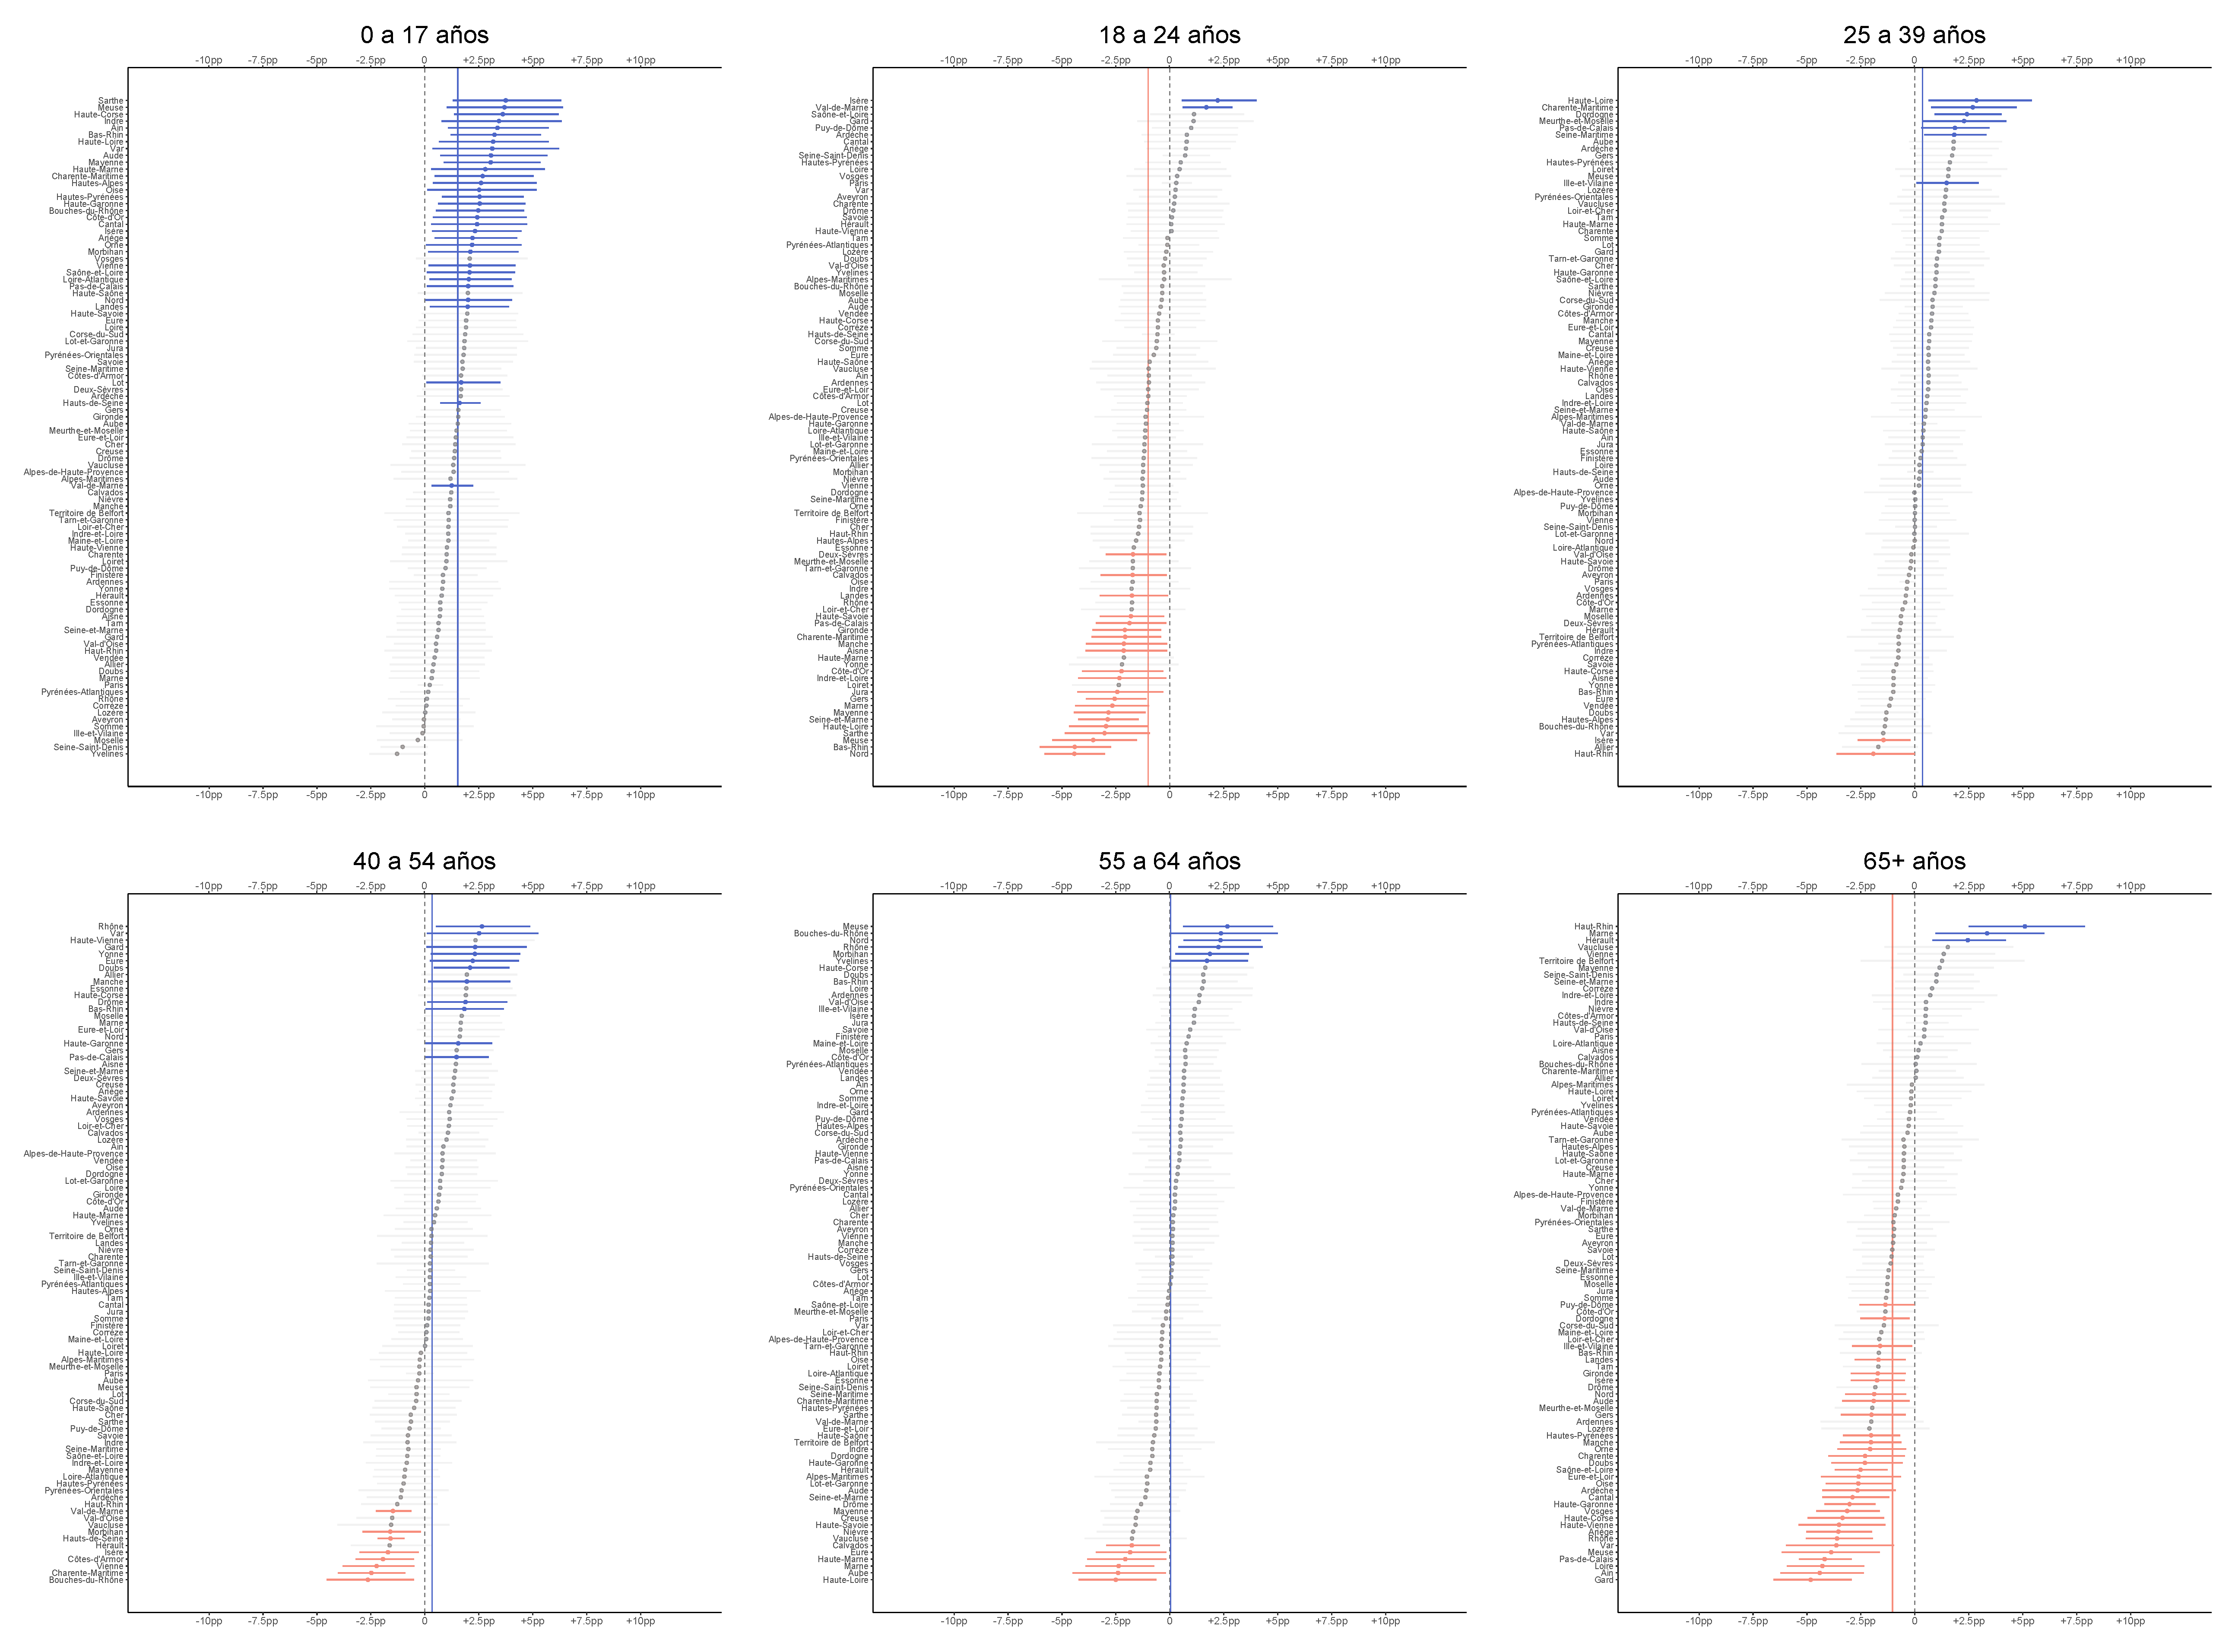
\includegraphics[width = 0.9\textwidth]{Figs/Efectos/Efectos_Edad_Modelo_H}
	\caption{Intervalos centrales de probabilidad al 95\%, 80\% y 50\% para los efectos del grupo de edad por departamento francés bajo el modelo H. Los departamentos se ordenan para cada categoría por magnitud del estimador puntual que es el efecto mediano. Las distribuciones de colores rosa o azul representan que el efecto es significativo al 95\%. Las lineas verticales representan el efecto promedio a través de los departamentos. Fuente: elaboración propia.}
	\label{fig:Efectos_Edad}
\end{figure}

Observando los dorlings de la \textbf{Figura \ref{fig:Dorling_Efectos_Edad}} vemos que los efectos significativos negativos del grupo de 18 a 24 años se ubican tanto al oeste francés como en el norte. Por otro lado, los mayores de 65 años parecen tener una mayor influencia en el sur del hexágono. 

\begin{figure}[H]
	\centering
	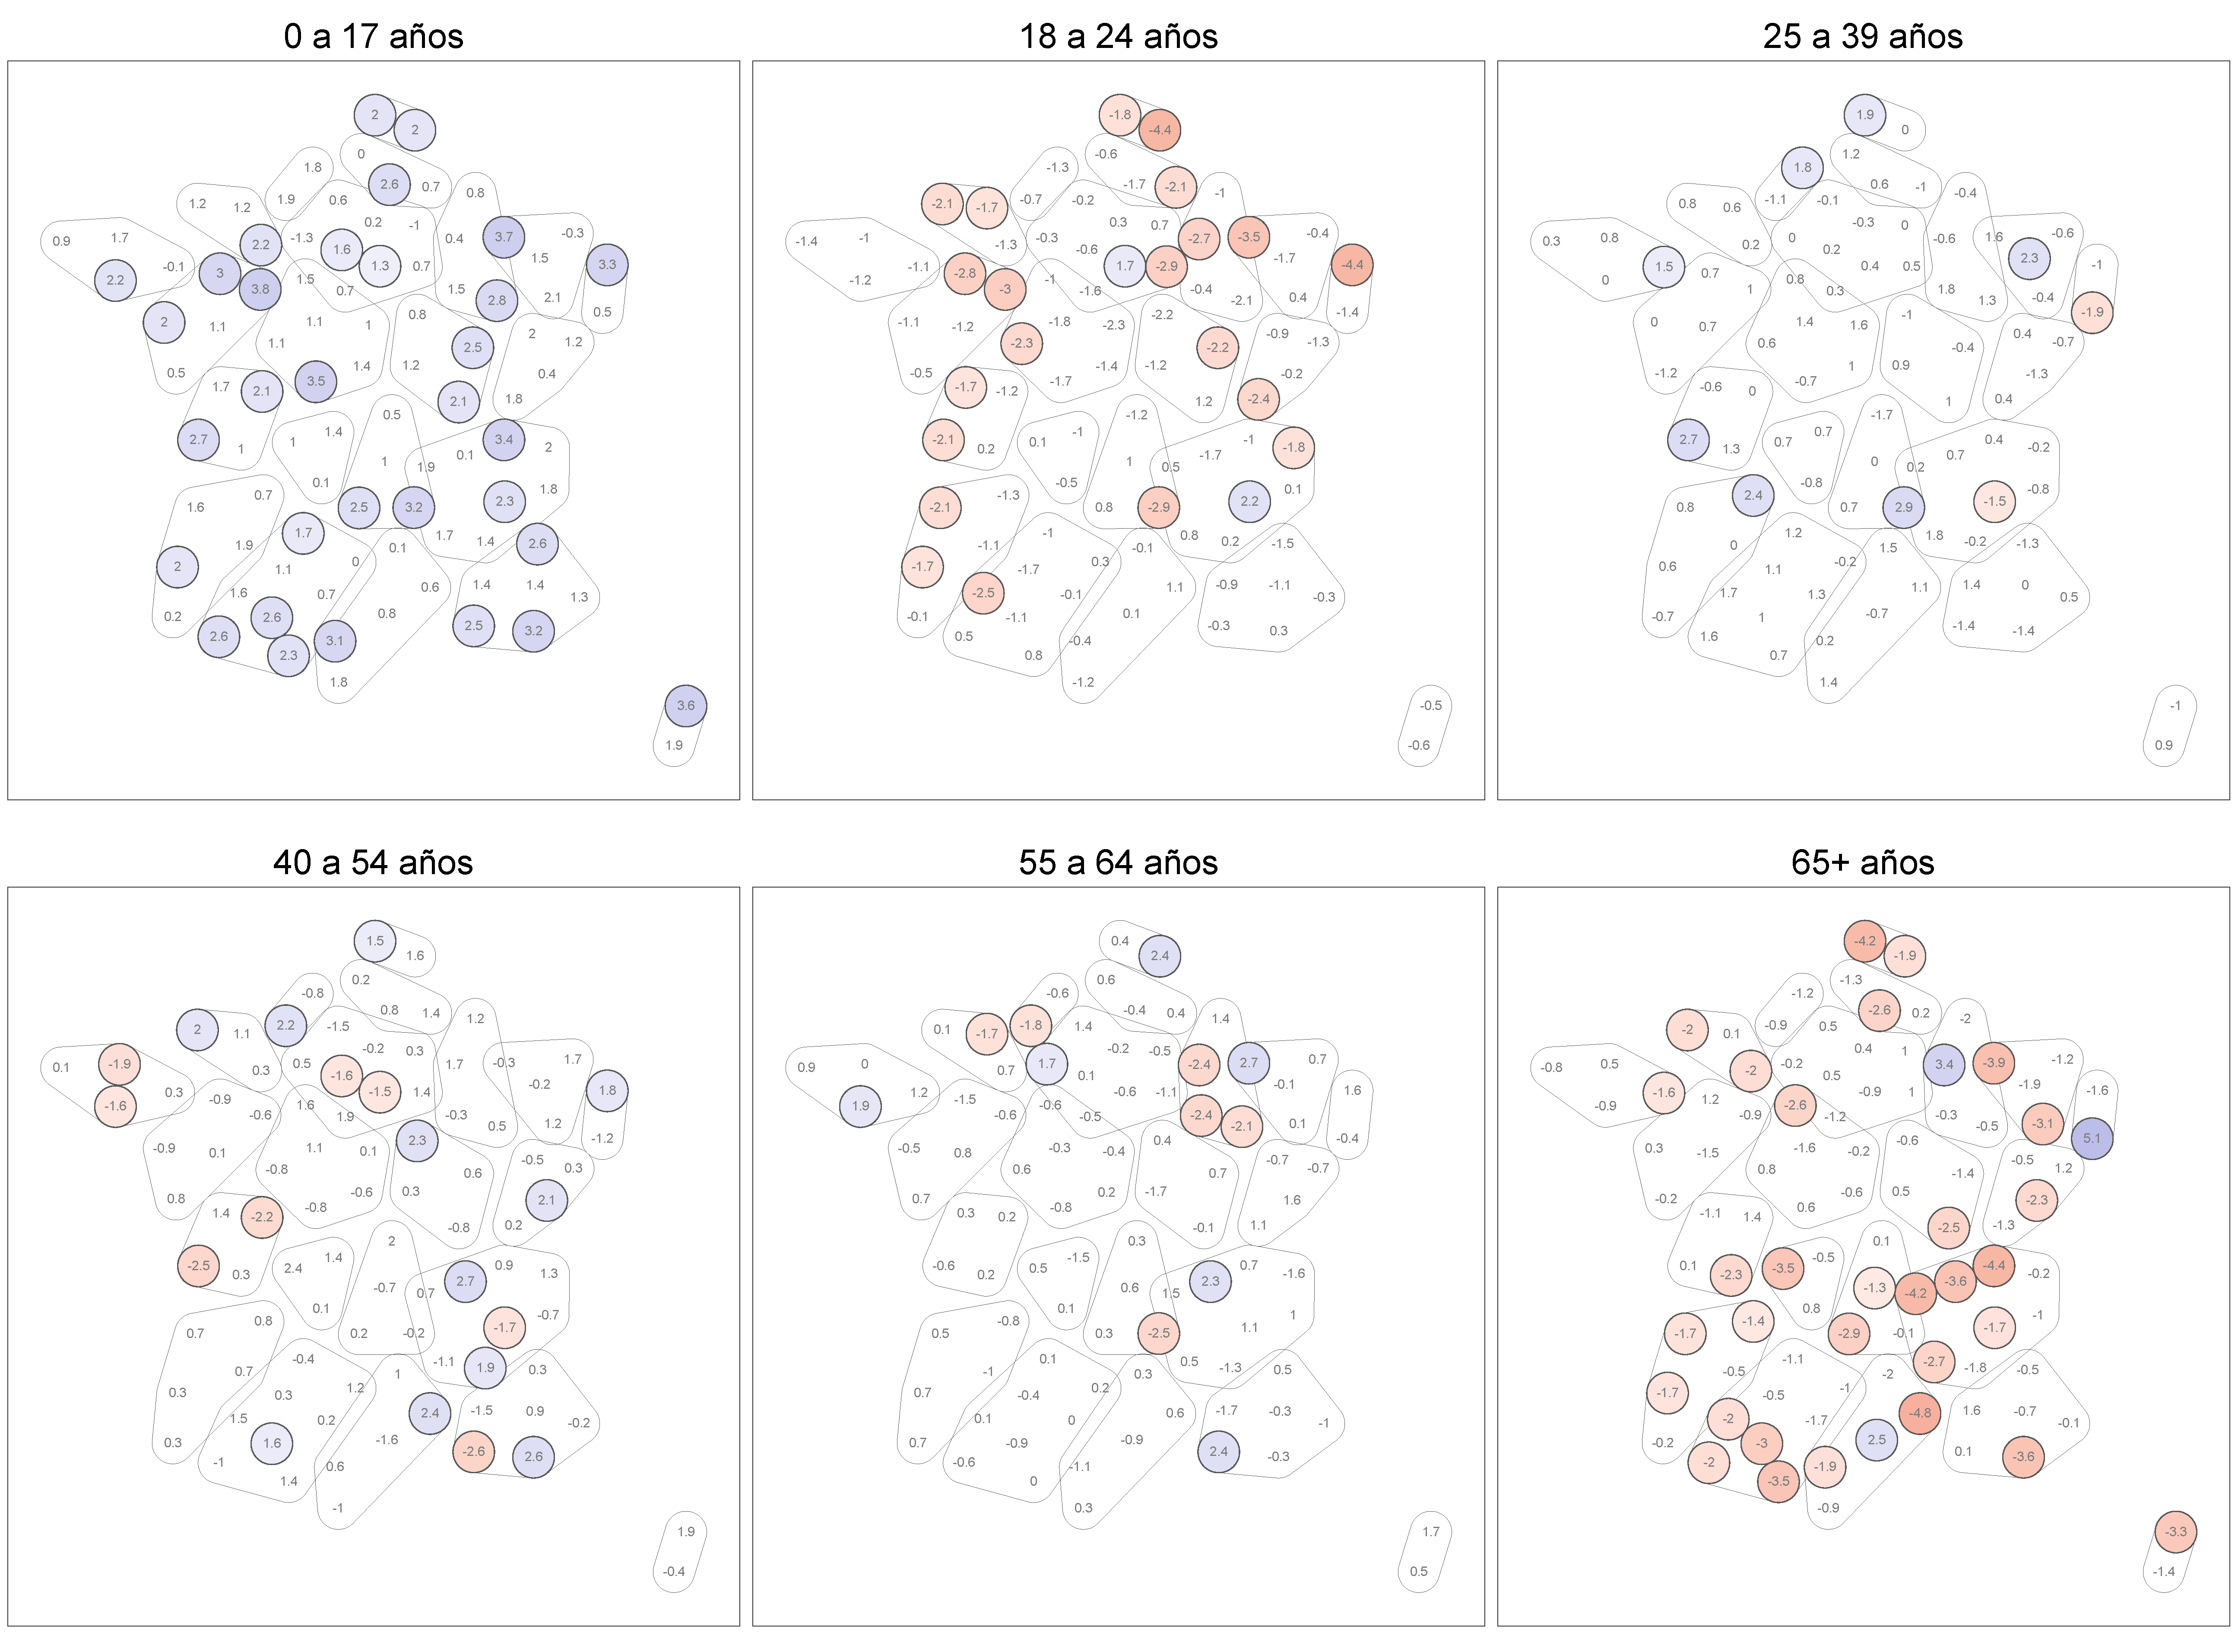
\includegraphics[width = 0.9\textwidth]{Figs/Efectos/Dorling_Efectos_Edad_Modelo_H}
	\caption{Estimaciones puntuales de los efectos del grupo de edad por departamento francés bajo el modelo H, solo se colorean los efectos significativos. Fuente: elaboración propia.}
	\label{fig:Dorling_Efectos_Edad}
\end{figure}

\subsection{Categorías dicotómicas}

Finalmente, podemos analizar los mapas de las variables dicotómicas, es decir las que tienen solo dos categorías: Sexo, Condición migratoria y (des)ocupaciones. En la \textbf{Figura \ref{fig:Mapa_Efectos_Dicotom}} vemos que la mayor presencia de inmigrantes como de mujeres parece inhibir el voto frontista. Por el contrario, las variables de desempleo no reflejan una geografía muy clara pero sí con efectos en ambos sentidos. Al observar los intervalos de la \textbf{Figura \ref{fig:Efectos_Dicotom}} para estas categorías, nos damos cuenta que existe mucha incertidumbre en las estimaciones. Esto parece continuar confirmándonos que el desempleo no resulta ser la variable con mayor poder explicativo, al menos en términos de configuraciones sociales de las comunas.\\ 

\begin{figure}[h]
	\centering
	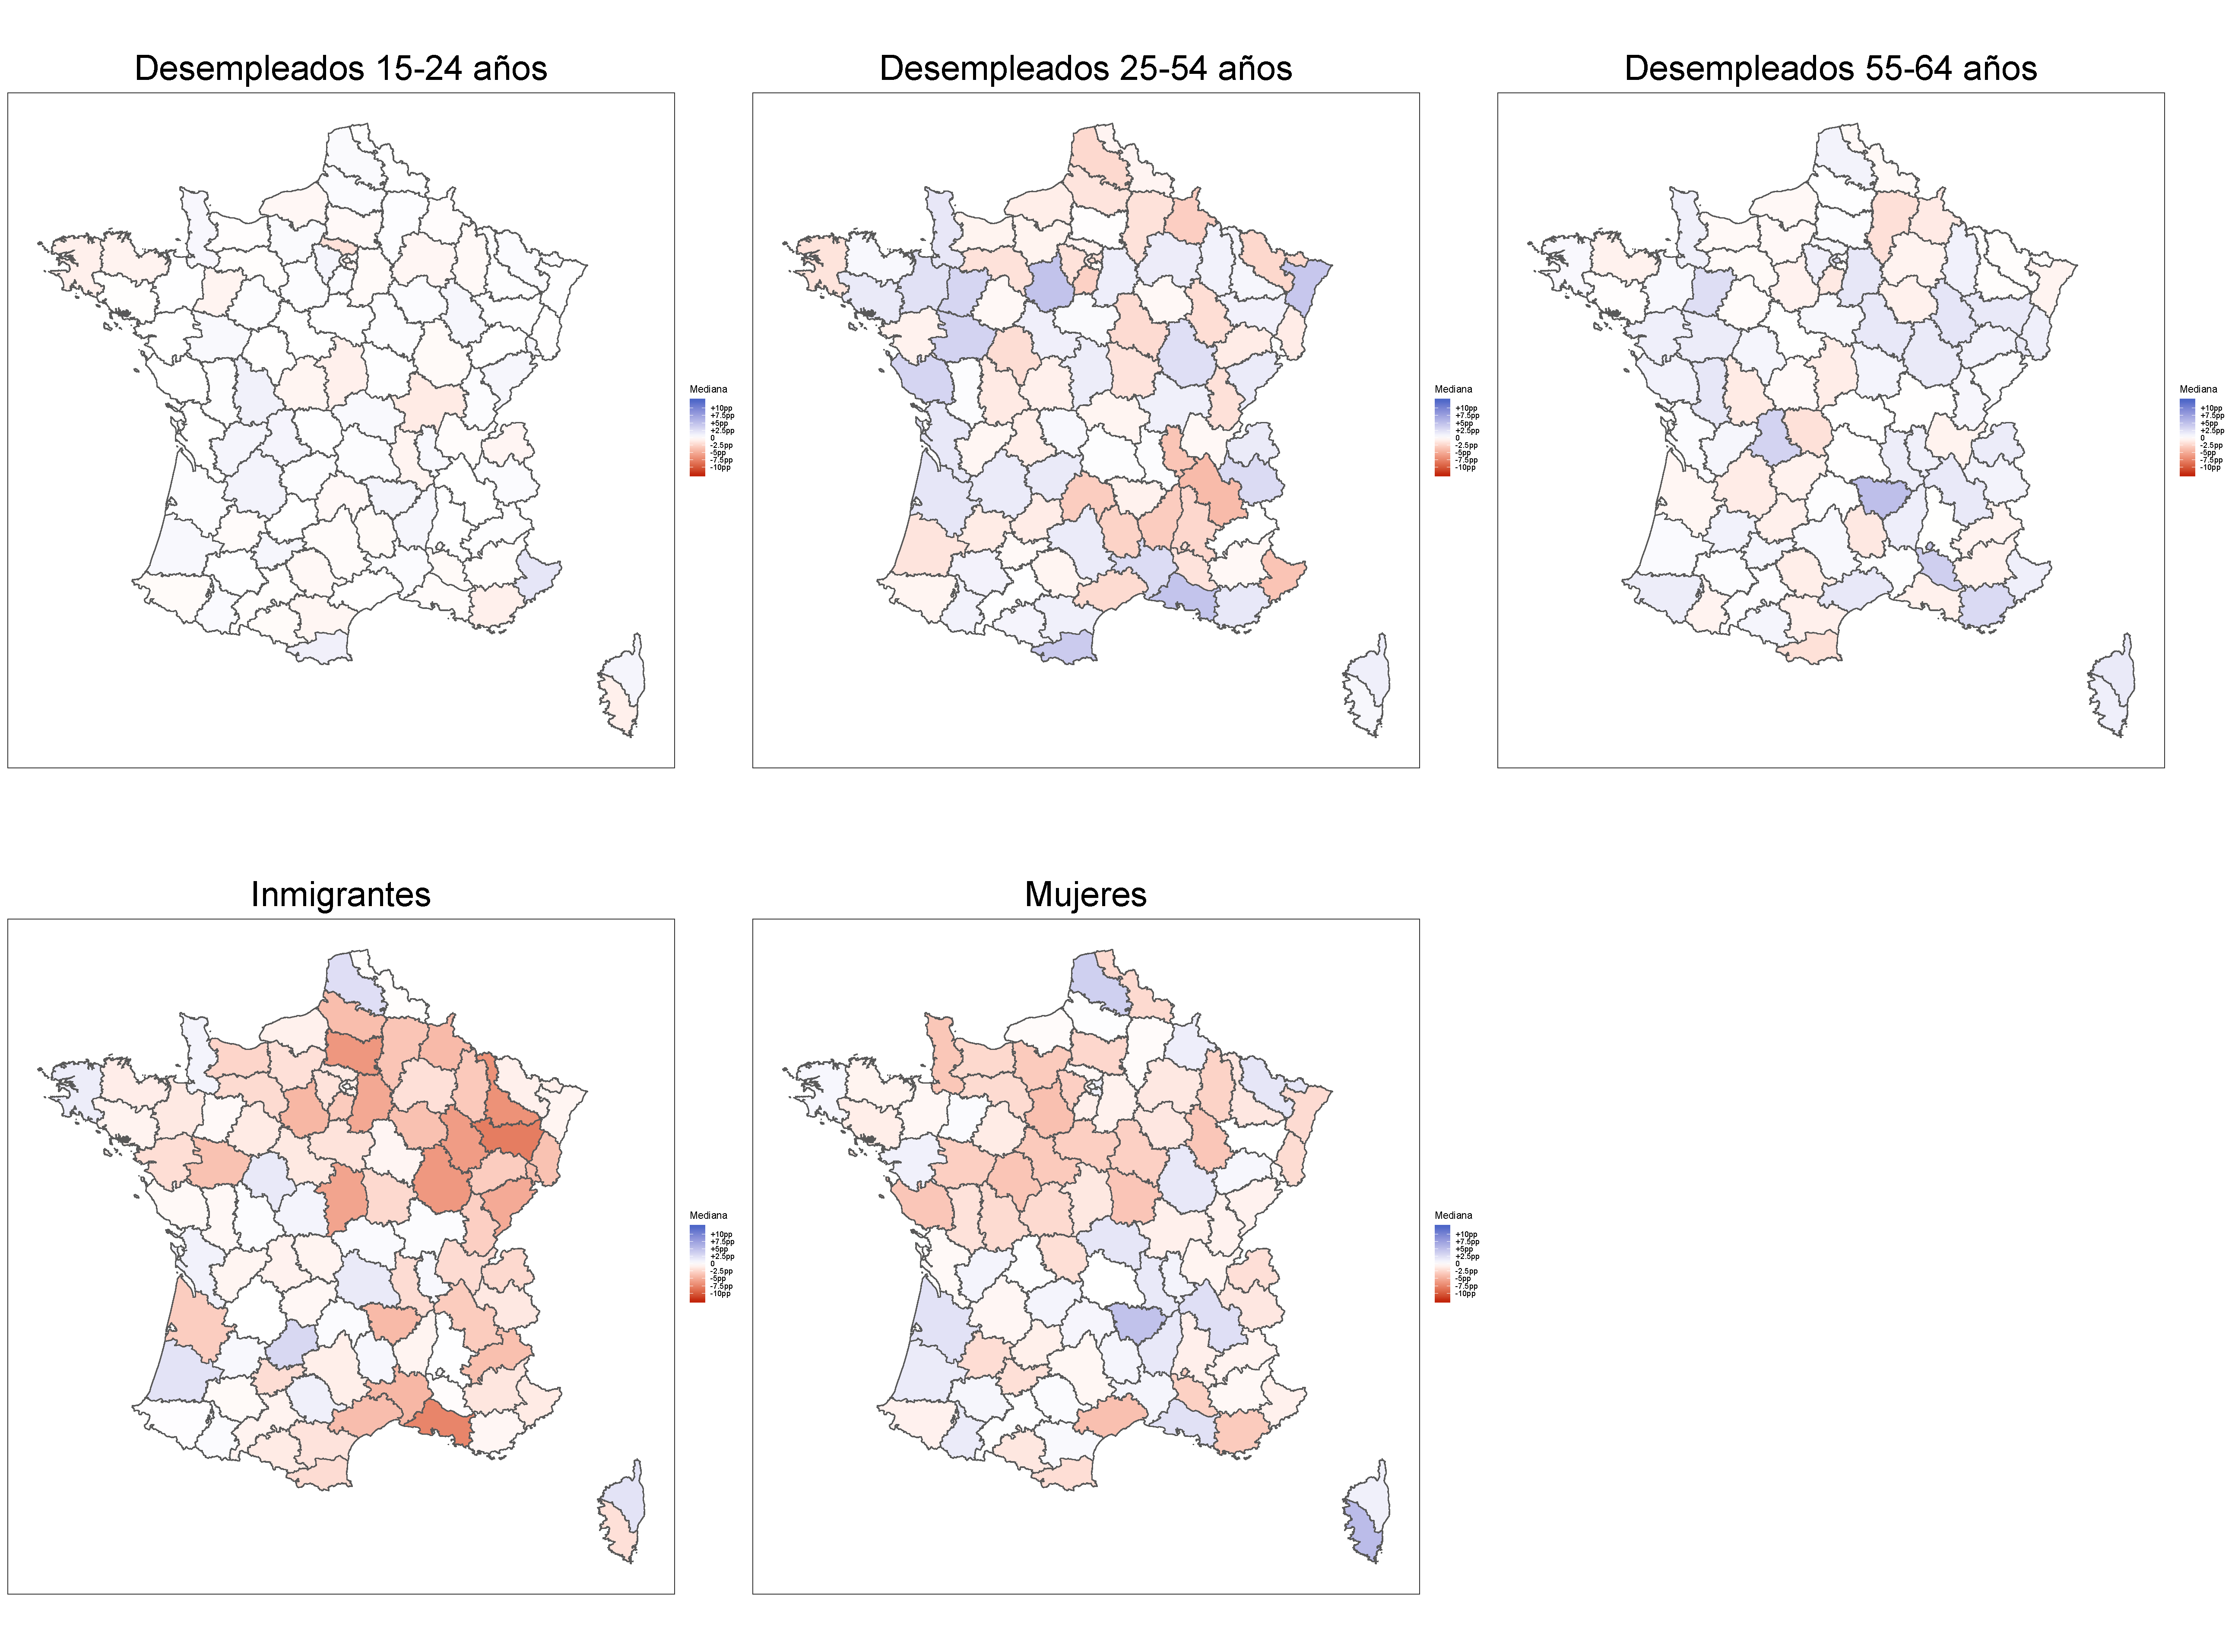
\includegraphics[width = 0.9\textwidth]{Figs/Efectos/Mapa_Efectos_Dicotom_Modelo_H}
	\caption{Estimaciones puntuales de los efectos de categorías dicotómicas por departamento francés bajo el modelo H. Fuente: elaboración propia con la cartografía de Open Street Map.}
	\label{fig:Mapa_Efectos_Dicotom}
\end{figure}

\begin{figure}[h]
	\centering
	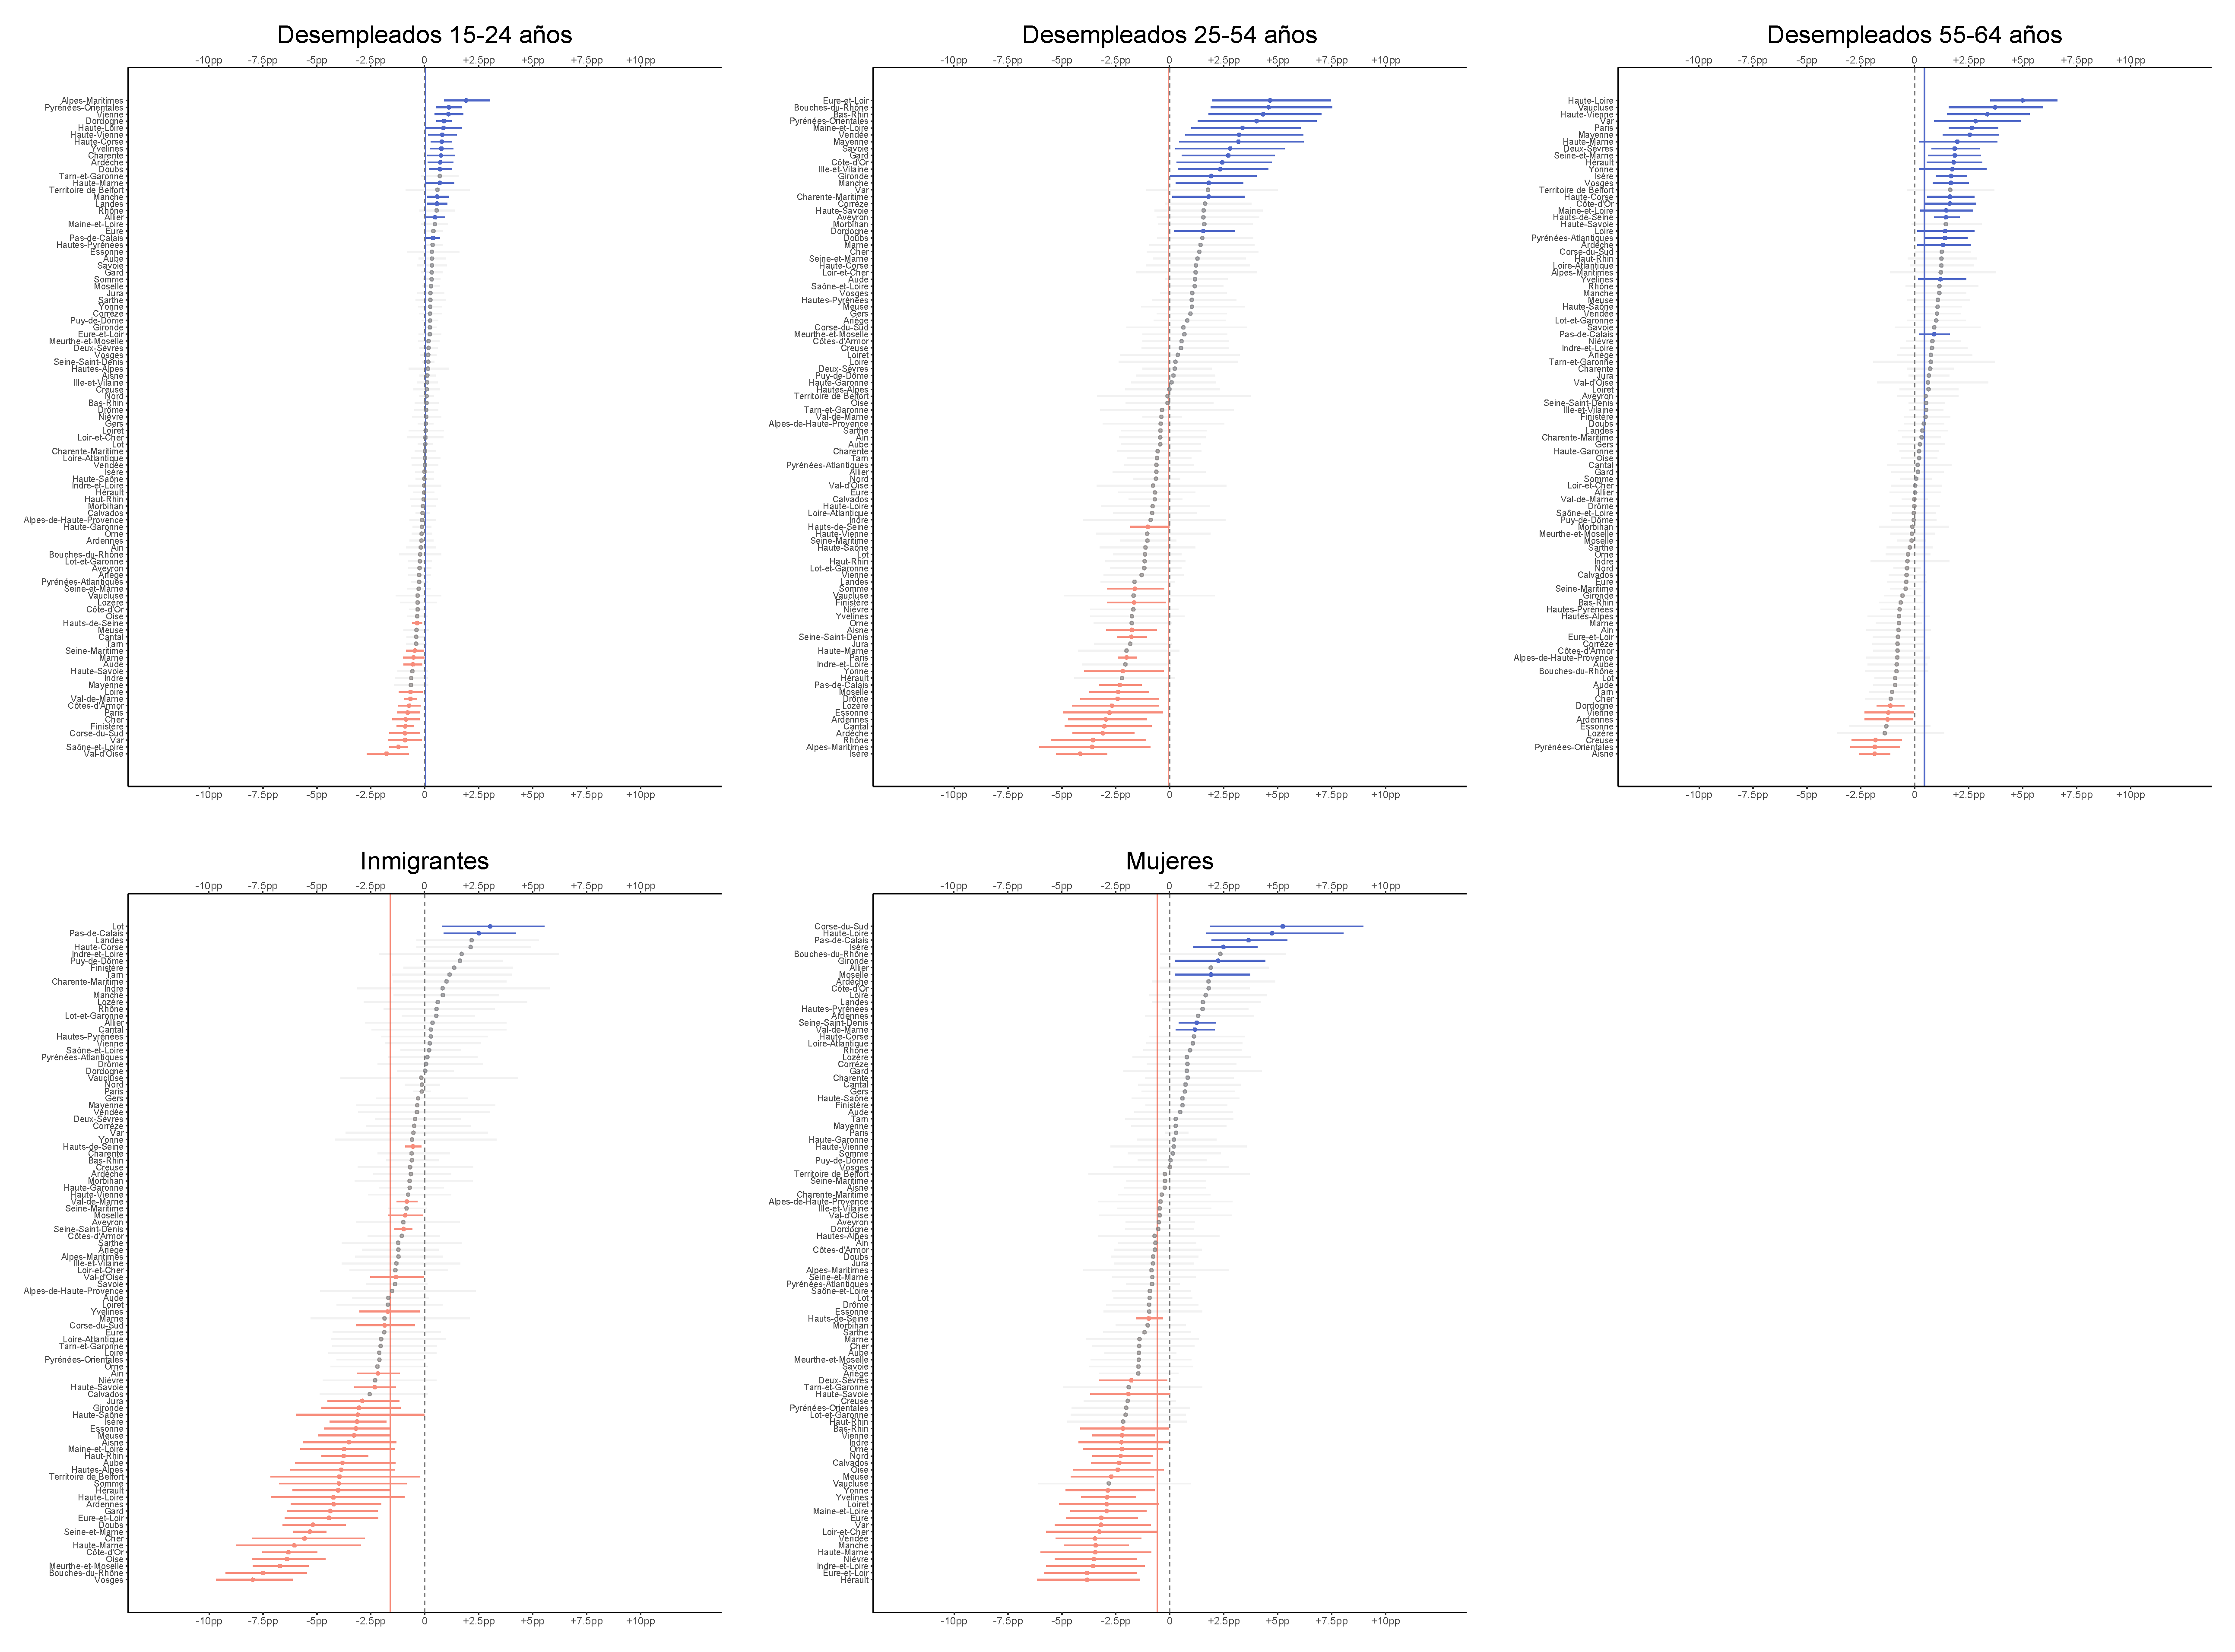
\includegraphics[width = 0.9\textwidth]{Figs/Efectos/Efectos_Dicotom_Modelo_H}
	\caption{Intervalos centrales de probabilidad al 95\%, 80\% y 50\% para los efectos de categorías dicotómicas por departamento francés bajo el modelo H. Los departamentos se ordenan para cada categoría por magnitud del estimador puntual que es el efecto mediano. Las distribuciones de colores rosa o azul representan que el efecto es significativo al 95\%. Las lineas verticales representan el efecto promedio a través de los departamentos. Fuente: elaboración propia.}
	\label{fig:Efectos_Dicotom}
\end{figure}

En el caso de la inmigración, las teorías del conflicto no parecen encontrar eco al observar los dorlings de la \textbf{Figura \ref{fig:Dorling_Efectos_Dicotom}}. Ciertamente aquí podríamos arriesgarnos a hablar de inferencia a nivel individual. Si una mayor proporción de inmigrantes adquieren derecho al voto, uno esperaría que no eligieran al partido NAP que resulta ser el FN. Por lo mismo, una mayor presencia de inmigrantes reduciría el voto frontista. Pero también existen las hipótesis que mencionan que el contacto con el inmigrante disminuye la xenofobia al comprobar que el otro no es tan diferente como se temía. En este sentido las explicaciones de un efecto indirecto de la presencia de inmigrantes parecerían más prometedoras que aquellas de xenofobia directa.\\

\begin{figure}[h]
	\centering
	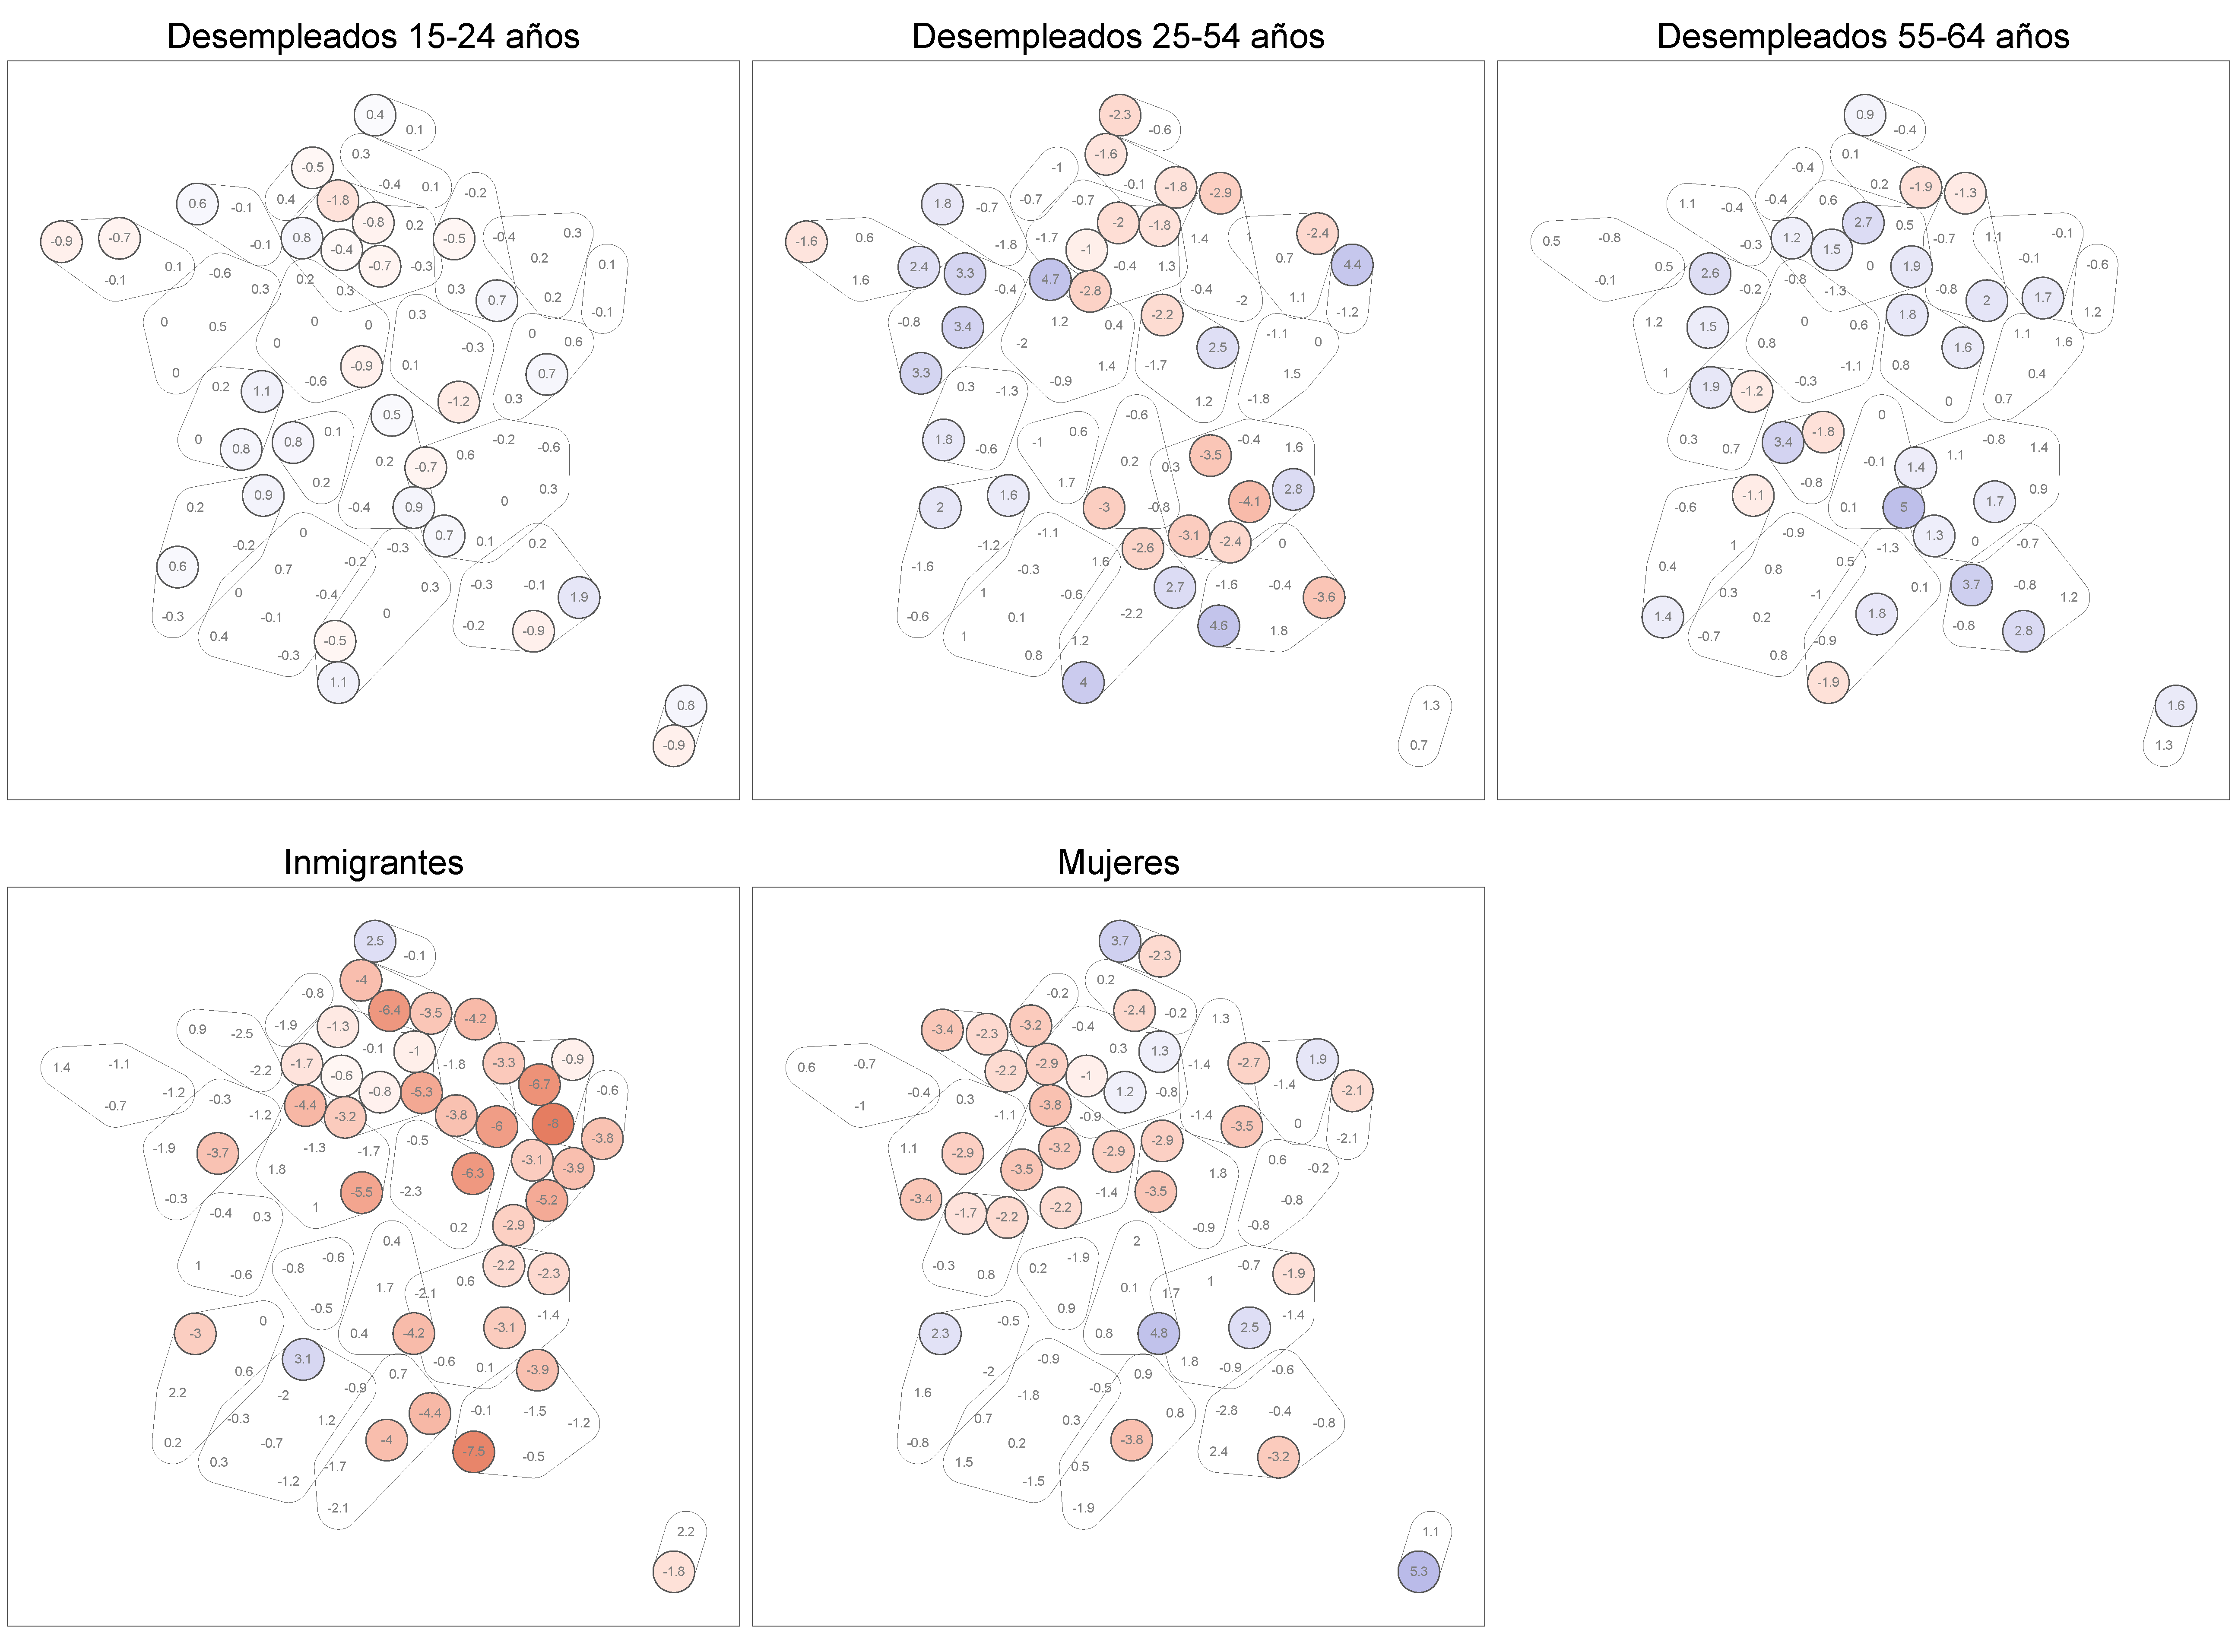
\includegraphics[width = 0.9\textwidth]{Figs/Efectos/Dorling_Efectos_Dicotom_Modelo_H}
	\caption{Estimaciones puntuales de los efectos de categorías dicotómicas por departamento francés bajo el modelo H, solo se colorean los efectos significativos. Fuente: elaboración propia.}
	\label{fig:Dorling_Efectos_Dicotom}
\end{figure}

Con base en este análisis gráfico procederé en el siguiente capítulo a resumir las conclusiones del estudio así como las primeras críticas que pudieran realizarse al modelo y, por lo mismo, algunas reflexiones sobre trabajo futuro y extensiones. 